\documentclass[leqno, openany]{memoir}
\setulmarginsandblock{3.5cm}{3.5cm}{*}
\setlrmarginsandblock{3cm}{3.5cm}{*}
\checkandfixthelayout

\usepackage{amsmath}
\usepackage{amssymb}
\usepackage{amsthm}
%\usepackage{MnSymbol}
\usepackage{bm}
\usepackage{accents}
\usepackage{mathtools}
\usepackage{tikz}
\usetikzlibrary{calc}
\usetikzlibrary{automata,positioning}
\usepackage{tikz-cd}
\usepackage{forest}
\usepackage{braket} 
\usepackage{listings}
\usepackage{mdframed}
\usepackage{verbatim}
\usepackage{physics}
\usepackage{spectralsequences} 
\usepackage{stackengine}
\usepackage{mathrsfs}
%\usepackage{/home/patrickl/homework/macaulay2}

%font
\usepackage[sc]{mathpazo}
\usepackage{eulervm}
\usepackage[scaled=0.86]{berasans}
\usepackage{inconsolata}
\usepackage{microtype}

%CS packages
\usepackage{algorithmicx}
\usepackage{algpseudocode}
\usepackage{algorithm}

% typeset and bib
\usepackage[english]{babel} 
\usepackage[utf8]{inputenc} 
\usepackage[T1]{fontenc}
\usepackage[backend=biber, style=alphabetic]{biblatex}
\usepackage[bookmarks, colorlinks, breaklinks]{hyperref} 
\hypersetup{linkcolor=black,citecolor=black,filecolor=black,urlcolor=black}

% other formatting packages
\usepackage{float}
\usepackage{booktabs}
\usepackage{enumitem}
\usepackage{csquotes}
\usepackage{titlesec}
\usepackage{titling}
\usepackage{fancyhdr}
\usepackage{lastpage}
\usepackage{parskip}

\usepackage{lipsum}

% delimiters
\DeclarePairedDelimiter{\gen}{\langle}{\rangle}
\DeclarePairedDelimiter{\floor}{\lfloor}{\rfloor}
\DeclarePairedDelimiter{\ceil}{\lceil}{\rceil}


\newtheorem{thm}{Theorem}[section]
\newtheorem{cor}[thm]{Corollary}
\newtheorem{prop}[thm]{Proposition}
\newtheorem{lem}[thm]{Lemma}
\newtheorem{conj}[thm]{Conjecture}
\newtheorem{quest}[thm]{Question}

\theoremstyle{definition}
\newtheorem{defn}[thm]{Definition}
\newtheorem{defns}[thm]{Definitions}
\newtheorem{con}[thm]{Construction}
\newtheorem{exm}[thm]{Example}
\newtheorem{exms}[thm]{Examples}
\newtheorem{notn}[thm]{Notation}
\newtheorem{notns}[thm]{Notations}
\newtheorem{addm}[thm]{Addendum}
\newtheorem{exer}[thm]{Exercise}

\theoremstyle{remark}
\newtheorem{rmk}[thm]{Remark}
\newtheorem{rmks}[thm]{Remarks}
\newtheorem{warn}[thm]{Warning}
\newtheorem{sch}[thm]{Scholium}


% unnumbered theorems
\theoremstyle{plain}
\newtheorem*{thm*}{Theorem}
\newtheorem*{prop*}{Proposition}
\newtheorem*{lem*}{Lemma}
\newtheorem*{cor*}{Corollary}
\newtheorem*{conj*}{Conjecture}

% unnumbered definitions
\theoremstyle{definition}
\newtheorem*{defn*}{Definition}
\newtheorem*{exer*}{Exercise}
\newtheorem*{defns*}{Definitions}
\newtheorem*{con*}{Construction}
\newtheorem*{exm*}{Example}
\newtheorem*{exms*}{Examples}
\newtheorem*{notn*}{Notation}
\newtheorem*{notns*}{Notations}
\newtheorem*{addm*}{Addendum}


\theoremstyle{remark}
\newtheorem*{rmk*}{Remark}

% shortcuts
\newcommand{\Ima}{\mathrm{Im}}
\newcommand{\A}{\mathbb{A}}
\newcommand{\N}{\mathbb{N}}
\newcommand{\R}{\mathbb{R}}
\renewcommand{\H}{\mathbb{H}}
\newcommand{\C}{\mathbb{C}}
\newcommand{\E}{\mathbb{E}}
\newcommand{\Z}{\mathbb{Z}}
\newcommand{\F}{\mathbb{F}}
\newcommand{\Q}{\mathbb{Q}}
\renewcommand{\k}{\Bbbk}
\renewcommand{\P}{\mathbb{P}}
\newcommand{\M}{\overline{M}}
\newcommand{\g}{\mathfrak{g}}
\newcommand{\h}{\mathfrak{h}}
\newcommand{\n}{\mathfrak{n}}
\renewcommand{\b}{\mathfrak{b}}
\newcommand{\ep}{\varepsilon}
\newcommand*{\dt}[1]{%
   \accentset{\mbox{\Huge\bfseries .}}{#1}}
\renewcommand{\abstractname}{Official Description}
\newcommand{\mc}[1]{\mathcal{#1}}
\newcommand{\T}{\mathbb{T}}
\newcommand{\mf}[1]{\mathfrak{#1}}
\newcommand{\mr}[1]{\mathrm{#1}}
\newcommand{\ms}[1]{\mathsf{#1}}
\newcommand{\ol}[1]{\overline{#1}}
\newcommand{\ul}[1]{\underline{#1}}
\newcommand{\wt}[1]{\widetilde{#1}}
\newcommand{\wh}[1]{\widehat{#1}}

\DeclareMathOperator{\Der}{Der}
\DeclareMathOperator{\Sq}{Sq}
\DeclareMathOperator{\Hom}{Hom}
\DeclareMathOperator{\colim}{colim}
\DeclareMathOperator{\coker}{coker}
\DeclareMathOperator{\End}{End}
\DeclareMathOperator{\ad}{ad}
\DeclareMathOperator{\ch}{ch}
\DeclareMathOperator{\Aut}{Aut}
\DeclareMathOperator{\Rad}{Rad}
\DeclareMathOperator{\supp}{supp}
\DeclareMathOperator{\sgn}{sgn}
\DeclareMathOperator{\spec}{Spec}
\DeclareMathOperator{\sign}{sign}
\DeclareMathOperator{\Vect}{Vect}
\DeclareMathOperator{\ind}{ind}
\DeclareMathOperator{\tind}{t-ind}

% Section formatting
\titleformat{\section}
    {\Large\sffamily\scshape\bfseries}{\thesection}{1em}{}
\titleformat{\subsection}[runin]
    {\large\sffamily\bfseries}{\thesubsection}{1em}{}
\titleformat{\subsubsection}[runin]{\normalfont\itshape}{\thesubsubsection}{1em}{}

\title{COURSE TITLE}
\author{Lectures by INSTRUCTOR, Notes by NOTETAKER}
\date{SEMESTER}

\newcommand*{\titleSW}
    {\begingroup% Story of Writing
    \raggedleft
    \vspace*{\baselineskip}
    {\Huge\itshape Algebraic Topology \\ Spring 2021}\\[\baselineskip]
    {\large\itshape Notes by Patrick Lei}\\[0.2\textheight]
    {\Large Lectures by Francesco Lin}\par
    \vfill
    {\Large \sffamily Columbia University}
    \vspace*{\baselineskip}
\endgroup}
\pagestyle{simple}

\chapterstyle{ell}


%\renewcommand{\cftchapterpagefont}{}
\renewcommand\cftchapterfont{\sffamily}
\renewcommand\cftsectionfont{\scshape}
\renewcommand*{\cftchapterleader}{}
\renewcommand*{\cftsectionleader}{}
\renewcommand*{\cftsubsectionleader}{}
\renewcommand*{\cftchapterformatpnum}[1]{~\textbullet~#1}
\renewcommand*{\cftsectionformatpnum}[1]{~\textbullet~#1}
\renewcommand*{\cftsubsectionformatpnum}[1]{~\textbullet~#1}
\renewcommand{\cftchapterafterpnum}{\cftparfillskip}
\renewcommand{\cftsectionafterpnum}{\cftparfillskip}
\renewcommand{\cftsubsectionafterpnum}{\cftparfillskip}
\setrmarg{3.55em plus 1fil}
\setsecnumdepth{subsection}
\maxsecnumdepth{subsection}
\settocdepth{subsection}

\begin{document}
    
\begin{titlingpage}
\titleSW
\end{titlingpage}

\thispagestyle{empty}
\section*{Disclaimer}%
\label{sec:disclaimer}

These notes were taken during lecture using the \texttt{vimtex} package of the
editor \texttt{neovim}.  Any errors are mine and not the instructor's.  In
addition, my notes are picture-free (but will include commutative diagrams) and
are a mix of my mathematical style and that of the instructor.  If you find any
errors, please contact me at \texttt{plei@math.columbia.edu}.

\section*{Acknowledgements}% \label{sec:acknowledgements}

I would like to thank Nicol\'as Vilches and Alex Xu for pointing out errors and
typos in these notes. I would also like to thank Alex for graciously offering
to teach everyone about the Dirac operator. 


\newpage


\tableofcontents

\chapter{Spectral Sequences}% \label{cha:spectral_sequences}

Our goal in this chapter will be to compute the homotopy groups of spheres, but
we are not algebraic topologists so we don't actually care about that. What we
know from the basic theory is that $\pi_i(S^n) = 0$ if $i < n$ and $\pi_n(S^n)
= \Z$, and this isomorphism is given by the degree. We also know that
$\pi_3(S^2) = \Z$ and is generated by the Hopf fibration $S^1 \hookrightarrow
S^3 \to S^2$. Note that this map is the attaching map of the $4$-cell of
$\C\P^2$.

There is an analogous decomposition $\H\P^2 = \mr{pt} \cup D^4 \cup D^8$. Then
we obtain a fibration $f \colon S^7 \to S^4$, which is an $S^3$-fibration.
Using the long exact sequence of the fibration, we see that $\pi_7(S^4)
\supseteq \Z$.

Next, we may consider $\mathbb{O}\P^2$, the octonionic projective plane. This
has a cell decomposition $\mr{pt} \cup D^8 \cup D^{16}$ and from this we obtain
a fibration $S^7 \hookrightarrow S^{15} \to S^8$ and compute that
$\pi_{15}(S^8) \supseteq \Z$. We should note, however, that $\mathbb{O}\P^2$ is
\textbf{not} the set of lines in $\mathbb{O}^3$ because the octonions do not
form an associative algebra. There is enough associativity to define some sort
of $\mathbb{O}\P^2$ but not $\mathbb{O}\P^n$ for $n \geq 3$. In fact, we will
prove that no space with the expected cohomology ring exists.

More generally, we can study $f \colon S^{2n-1} \to S^n$ as follows: Consider
the mapping cone $S^n \cup_f D^{2n} \eqqcolon C_f$. Then the cohomology is \[
    H^i(C_f) = \begin{cases} \Z & i = 0, n, 2n \\ 0 & \text{otherwise}
    \end{cases}. \] Then choose generators $\alpha \in H^n, \beta \in H^{2n}$.
    We then have $\alpha^2 = H(f) \beta \in H^{2n}$ for some integer $H(f)$,
    called the \textit{Hopf invariant}.

\begin{exm} The attaching maps of $\C\P^2, \H\P^2, \mathbb{O}\P^2$ all have
$H(f) = 1$. This implies that $H^* = \Z[\alpha]/(\alpha^3)$.  \end{exm}

We know that if $f,g$ are homotopic, then $H(f) = H(g)$ because the mapping
cones are homotopy equivalent. Then we obtain a homomorphism $H \colon
\pi_{2n-1}(S^n) \to \Z$. Note that when $n$ is odd, we have $\alpha^2 =
-\alpha^2$ by graded commutativity, and so $H(f) = 0$.

\begin{exm} If $n = 2k$ is even, there exists $f \colon S^{4k-1} \to S^{2k}$
with $H(f) = 2$.  \end{exm}

Now given a pointed space $(X,e)$ define $J_2(X) = X \times X / (x,e) \sim
(e,x)$. This is somewhere between the product and the smash product, and so
$J_2(S^{2k})$ is a CW complex with a single cell in dimensions $0, 2k, 4k$.

\begin{exer} The attaching map of the $4k$-cell has $H(f) = 2$.  \end{exer}

\begin{cor} $\pi_{4k-1}(S^{2k})$ admits a $\Z$-summand. This is because $H$
surjects onto either $2\Z$ or $\Z$, and so it splits.  \end{cor}

We have the following results:

\begin{thm}[Serre] $\pi_i(S^n)$ is a finitely generated abelian group. It has
rank $1$ if $i = n$ or $i = 2n-1$ and $n$ is even.  \end{thm}

\begin{thm}[Adams] If $[f] \in \pi_{2n-1}(S^n)$ with $H(f) = 1$, then $n =
2,4,8$.  \end{thm}

\begin{rmk} This is related to the following. Suppose $\R^n$ admits the
    structure of a division algebra. This is a bilinear map $* \colon \R^n
    \otimes \R^n \to \R^n$ that is invertible for $a \neq 0$. Then $n =
    1,2,4,8$. We will prove this result using K-theory.  \end{rmk}

\section{The Simplest Case}% \label{sec:the_simplest_case}

Here, we will consider $\pi_{n+1}(S^n)$ for $n \geq 3$. By the Freudenthal
suspension theorem, we have maps \[ \pi_3(S^2) \xrightarrow{\Sigma} \pi_4(S^3)
\xrightarrow[\sim]{\Sigma} \pi_5(S^4) \to \cdots \] Therefore the group we need
to compute is $\pi_4(S^3)$. The key strategy is to exploit the interaction
between homotopy and homology. Here, we will consider the \textit{Hurewicz map}
\[ h \colon \pi_n(X) \to H_n(X) \qquad [f] \mapsto f_* [S^n]. \]

\begin{thm}[Hurewicz] Suppose $n \geq 2$ and $X$ is $(n-1)$-connected. Then
$\wt{H}_0(X) = H_1(X) = \cdots = H_{n-1}(X) = 0$ and $h \colon \pi_n(X) \simeq
H_n(X)$.  \end{thm}

\begin{rmks} When $n = 1$, $H_1(X)$ is the abelianization of $\pi_1(X)$. Also,
there is a relative version of the Hurewicz theorem.  \end{rmks}

\begin{proof}[Sketch of Proof] We can assume $X$ is a CW complex with a single
    $0$-cell and no cells in dimension $1, \ldots, n-1$. Then we can replace
    $X$ with $X^{n+1}$, so we can write \[ X = \qty( \bigvee_{\alpha}
    S_{\alpha}^n ) \cup_{\beta} D_{\beta}^{n+1}. \] By homotopy excision, we
    have \[ \pi_n(X) = \mr{coker}(d \colon \pi_{n+1}(X, X^n) \to \pi_n(X^n)) \]
and this is exactly $C_{n+1}(X) \to C_n(X) \to 0$.  \end{proof}

Our strategy to compute $\pi_4(S^3)$ will be to construct a space whose
homology is $\pi_4(S^3)$. Recall that $\pi_3(K(\Z, 3)) = \Z$ by definition, and
so consider $f \colon S^3 \to K(\Z, 3)$ be a generator. Then $f_* \colon
\pi_3(S^3) \xrightarrow{\sim} \pi_3(K(\Z, 3))$ is an isomorphism. Now we can
turn $f$ into a fibration $F \hookrightarrow S^3 \to K(\Z, 3)$. Considering the
long exact sequence of the fibration, we have \[ 0 \to \pi_4(F) \to \pi_4(S^3)
\to 0 \to \pi_3(F) \to \pi_3(S^3) \to \pi_3(K(\Z, 3)) \to \cdots \] and
therefore $\pi_0(F) = \pi_1(F) = \pi_2(F) = \pi_3(F) = 0$. We also have
$\pi_n(F) \cong \pi_n(S^3)$ for $n \geq 4$. In particular, we have $\pi_4(S^3)
= \pi_4(F) = H_4(F)$.If we can understand $F$ in some reasonable way, then we
will be done.

If we turn $F \hookrightarrow S^3$ into a fibration, then the homotopy fiber is
now a $K(\Z, 2) = \C\P^{\infty}$. Now we have a fibration and we know the
homology of both $S^3$ and $\C\P^{\infty}$, so the question is to compute $H_4$
from the information we have.

\begin{quest} Given $F \hookrightarrow E \to B$ a fibration, is there a
relationship between $H_*(B), H_*(E), H_*(F)$?  \end{quest}

Recall that in the case when $E \cong F \times B$ this relation is given by the
K\"unneth formula. Here, we see that $C_*(E) = C_*(F) \otimes C_*(B)$ as chain
complexes, and so we reduce the problem to homological algebra. This gives us

\begin{thm} Let $R$ be a principal ideal domain. Then there is a natural short
    exact sequence \[ 0 \to \bigoplus H_i(F,R) \otimes H_{n-i}(B, R) \to H_n(F
    \times B, R) \to \bigoplus \mr{Tor}^1_R(H_i(F,R), H_{n-1-i}(B, R)) \to 0 \]
    and this sequence splits (but not naturally).  \end{thm}

\begin{exm} We can compute that $H_*(S^1 \times S^2) = \Z$ in dimensions
$0,1,2,3$.  \end{exm}

However, we note that the Kunneth theorem does not hold for fibrations in
general. To see this, consider the Hopf fibration.

\begin{exm} Consider the fibration $K(\Z, n-1) \hookrightarrow * \to K(\Z, n)$.
    Both the base and fiber have nontrivial homology, but clearly the total
    space is contractible, so it has trivial homology. In both examples,
    $H_*(E)$ is \textbf{smaller} than what we would get from K\"unneth.
\end{exm}

\section{Spectral Sequences}% \label{sec:spectral_sequences}

\begin{defn} A \textit{spectral sequence} is a sequence $(E^r, d_r)$, where
$E^r$ is an $R$-module and $d_r \colon E^r \to E^r$ is a differential. In
addition, we require that $E^{r+1} = H_*(E^r, d_r)$.  \end{defn}

\begin{rmk} Note that $(E^r, d_r)$ determines $E^{r+1}$, but not $d_{r+1}$ in
general.  \end{rmk}

Now assume that $d_r = 0$ for $r \gg 0$ so that $E^r = E^{r+1} = \cdots
\eqqcolon E^{\infty}$.

\begin{defn} We say that $(E^r, d_r) \Rightarrow G$, or $(E_r, d_r)$
    \textit{converges to $G$}, if $G$ admits a filtration \[ 0 = G_{-1} \subset
    G_0 \subset G_1 \subset \cdots \subset G_n = G \] such that $\bigoplus G_i
    / G_{i-1} \cong E^{\infty}$.  \end{defn}

\begin{rmk} This says that $G$ is recovered by $(E^r, d_r)$ up to extension
problems.  \end{rmk}

\begin{exm} Consider a short exact sequence $0 \to A_* \to C_* \to C_*/A_* \to
    0$ of chain complexes. Then we will see that there is a spectral sequence
    with $E^1 = H_*(A) \oplus H_*(C/A)$ and $(E^r, d_r) \Rightarrow H_*(C)$. 

    First, consider the long exact sequence in homology. If we consider the
    boundary homomorphism $\delta_i$, we obtain a long exact sequence \[ 0 \to
    \operatorname{coker} \delta_{i+1} \to H_i(C) \to \ker \delta_i \to 0. \]
    Now define $E^1 = H_*(A) \oplus H_*(C / A)$ with $d_1 = \bigoplus
    \delta_i$. Then we have \[ H_*(E^1, d_1) = \qty( \bigoplus \ker \delta_i )
    \oplus \qty(\bigoplus \operatorname{coker} \delta_i) \eqqcolon E^2, \] as
desired. Then we let $d_2 = 0$.  \end{exm}

This tells us that if $H_*(A) = H_*(C/A) = 0$, then $H_*(C) = 0$. Also, if
$H_*(C) = 0$, then $H_*(A) \cong H_*(C/A)$ with a shift.

\begin{thm}[Serre] Let $F \hookrightarrow E \to B$ be a fibration and let
$\pi_1(B) = 1$. Then there is a spectral sequence $(E^r, d_r)$ such that
\begin{itemize} \item $E^2 \cong H_*(B; H_*(F))$; \item $(E^r, d_r) \Rightarrow
H_*(E)$.  \end{itemize} \end{thm}

Note here that we need to define what it means to converge in this setting.
Also, note that $E^3$ is smaller than $E^2$, so this formalizes the notion that
$H_*(E)$ is smaller than what we naively expect.

\begin{rmk} We actually do not know what $d_2$ is, so it is impossible to
compute the homology in general.  \end{rmk}

Fortunately, there is more structure: \begin{itemize} \item $E^r_{*,*}$ is
    bigraded.  \item $d_r$ has bidegree $(-r, r-1)$.  \item $E_{p,q}^2 = H_p(B;
    H_q(F))$.  \item $E_{p,q}^r = E_{p,q}^{\infty}$ for $r \gg 0$ depending on
    $p,q$.  \item $H_n(E)$ has a filtration with associated graded $\bigoplus
    E_{i, n-i}^{\infty}$.  \end{itemize}

\begin{exm} Consider the example $S^1 \hookrightarrow * \to \C\P^{\infty}$.
    Then we know that $E_{p,q}^2 = H_p(B, H_q(S^1))$ and therefore the spectral
    sequence is \begin{center}
        \begin{sseqdata}[classes={draw=none},name=cpinf,homological Serre
            grading,xscale=1.8, y axis gap = 2em] \class["H_0(B)"](0,0)
            \class["H_1(B)"](1,0) \class["H_2(B)"](2,0) \class["H_3(B)"](3,0)
            \class["\ldots"](4,0) \class["H_0(B)"](0,1) \class["H_1(B)"](1,1)
            \class["H_2(B)"](2,1) \class["H_3(B)"](3,1) \class["\ldots"](4,1)
        \d[->]2(2,0) \d[->]2(3,0) \d[->]2(4,0) \end{sseqdata}
    \printpage[name=cpinf,page=2, grid=chess] \end{center} This gives us
    $\delta_i \colon H_{2+i}(B) \to H_i(B)$, and so $d_3$ has degree $(-3, 2)$
    and thus it has to be zero. By degree reasons, we see that $E^4 = E^3$ and
    $d_4 = 0$, so $E^{\infty} = E^3$. Then, the total space is a point, and so
    writing the $E^3$-page \begin{center}
        \begin{sseqdata}[classes={draw=none},name=cpinf3,homological Serre
            grading,xscale=1.8, y axis gap = 2em] \class["\coker
            \delta_0"](0,1) \class["\coker \delta_1"](1,1) \class["\coker
            \delta_2"](2,1) \class["H_0(B)"](0,0) \class["H_1(B)"](1,0)
        \class["\ker \delta_0"](2,0) \class["\ker \delta_1"](3,0) \class["\ker
    \delta_2"](4,0) \end{sseqdata} \printpage[name=cpinf3, page=3, grid=chess]
\end{center} we see that $H_0(B) = \Z, H_1(B) = 0$ and that $\ker \delta_i =
\operatorname{coker} \delta_i = 0$. This recovers the usual computation of the
homology of $\C\P^{\infty}$.  \end{exm}

\begin{exm} We want to compute $H_*(\Omega S^2)$. Here, we will use the fiber
    sequence $\Omega S^2 \hookrightarrow * \to S^2$. Here, we know that
    $E_{p,q}^2 = H_p(S^2, H_q(F))$, so the $E^2$-page looks like \begin{center}
        \begin{sseqdata}[classes={draw=none}, name=omegas2, homological Serre
            grading, xscale=1.5, y axis gap = 2em] \class["H_0(F)"](0,0)
            \class["H_1(F)"](0,1) \class["H_2(F)"](0,2) \class["H_3(F)"](0,3)
            \class["H_0(F)"](2,0) \class["H_1(F)"](2,1) \class["H_2(F)"](2,2)
            \class["H_3(F)"](2,3) \d["g_0", ->]2(2,0) \d["g_1", ->]2(2,1)
            \d["g_2", ->]2(2,2) \end{sseqdata} \printpage[name=omegas2, page=2,
            grid=chess] \end{center} Then the $E^3$-page looks like
            \begin{center} \begin{sseqdata}[classes={draw=none}, name=omegas23,
                homological Serre grading, xscale=1.5, y axis gap = 2em]
                \class["H_0(F)"](0,0) \class["\coker g_0"](0,1) \class["\coker
                g_1"](0,2) \class["\coker g_2"](0,3) \class["\ker g_0"](2,0)
                \class["\ker g_1"](2,1) \class["\ker g_2"](2,2) \class["\ker
            g_3"](2,3) \end{sseqdata} \printpage[name=omegas23, page=3,
        grid=chess] \end{center} and the differential has degree $(-3,2)$, so
        $d_3 = 0$. This implies that $E^{\infty} = E_3$, and so the associated
        graded pieces are $\Z,0,0,0$. We see that $H_0(F) = \Z$ and each $g_i$
        is an isomorphism. This tells us that $H_i(\Omega S^2) \cong \Z$ for
        all $i$.  \end{exm}

\begin{exm} We can enhance this example to $\Omega S^n \hookrightarrow * \to
    S^n$. In this case, the first possible nontrivial differential is $d_n$,
    which has degree $(-n, n-1)$. This gives us $E^{n+1} = E^{\infty}$ for
    degree reasons, so we can compute \[ H_i(\Omega S^n) = \begin{cases} \Z &
    (n-1) \mid i \\ 0 & \text{otherwise}.  \end{cases} \] because $\delta_i
\colon H_i(F) \to H_{i+n-1}(F)$ is an isomorphism.  \end{exm}

Recall that our goal was to study $\C\P^{\infty} \hookrightarrow F \to S^3$.
However, we cannot compute this yet, so we will need to introduce even more
structure. To do this, we will need to do some homological algebra.

Considered a filtered chain complex, which is an abelian group $C$ with a map
$d \colon C \to C$ such that $d^2 = 0$. To this, we attach a filtration $0 =
F_{-1} C \subseteq F_0 C \subseteq \cdots \subseteq F_n C = C$ such that $d(F_i
C) \subseteq F_i C$.

\begin{rmk} $(F_i C, D)$ is a subcomplex of $C$.  \end{rmk}

Now if $X$ is a topological space with filtration $X_{-1} = \emptyset \subset
X_0 \subset \cdots \subset X_n = X$. Then if $C_*(X)$, we can choose $F_i C =
C_*(X_i)$, and this is a filtration.

Given $(C,d)$ and a filtration, we can associate two objects: \begin{enumerate}
    \item $\mr{Gr}_* C = \bigoplus F_i C / F_{i-1} C$, the \textit{associated
        graded} complex. Then we may consider the homology of this complex,
        which is a graded object.  \item Given a subcomplex $(F_i C, d)
        \hookrightarrow (C,d)$, we have a map $H(F_i C, d) \to H(C, d)$. The
        image of this is $F_i H(C,d)$, so we get a filtration on the homology
        $H(C)$. So then we obtain a graded \[ \mr{Gr}_* H(C,d) = \bigoplus F_i
    H(C) / F_{i-1} H(C). \] \end{enumerate} Now we want to consider
    therelationship between the two. Note that the first one is bigger, because
    $x \in \mr{Gr}_i C$ is a cycle if $\dd{x} \in F_{i-1} C$, while $x \in C$
    is a cycle if $\dd{x} = 0$.

\begin{thm}[Leray] There exists a spectral sequence $(E_*^r, d_r)$ such that
    \begin{itemize} \item $E_*^1 \cong H_* (\mr{Gr}_* C, d_0)$.  \item The
        spectral sequence converges to $H(C)$, or more precisely, $E_*^{\infty}
        \cong \mr{Gr}_* H(C)$.  \end{itemize} \end{thm}

\begin{proof} Consider the group \[ E_p^r = \frac{F_p C \cap \dd^{-1}(F_{p-r}
    C)}{(F_{p-1} C \cap \dd^{-1} F_{p-r} C) + (F_p C \cap \dd(F_{q+r-1} C))}.
    \] Notice that \begin{align*} E_p^0 &= \frac{F_p C}{F_{p-1} C + d(F_{p-1}
    C)} = \frac{F_p C}{F_{p-1} C} \\ E_p^1 &= \frac{F_p C \cap d^{-1} F_{p-1}
C}{F_{p-1}C + d(F_p C)} = H_p(\mr{Gr}_* C, \dd_0) \\ E_p^{\infty} &= \frac{F_p
C \cap \ker \dd}{(F_{p-1} \cap \ker d) + (F_p C \cap \Im d)} = \frac{F_p
H(C)}{F_{p-1} H(C)}, \end{align*} so all the groups are as expected. For the
differential, we define $\dd{r} \colon E_*^r \to E_r^*$ and in fact $\dd_r
\colon E_p^r \to E_{p-r}^r$ and thus has degree $-r$. Choose $\alpha \in E_p^r$
and choose $a \in F_p C \cap \dd^{-1}(F_{p-r} C)$ a representative. Then
$\dd{\dd{a}} = 0$ implies that $\dd{a} \in \dd^{-1}(0) \subset
\dd^{-1}(F_{p-2r} C)$ and therefore $\dd{a} \in F_{p-r} C \cap d^{-1}(F_{p-2r}
C)$. Therefore $\dd{a}$ defines an element in $E_{p-r}^r$, so we set $\dd^r
\alpha = [\dd{a}] \in E_{p-r}^r$.

    The things that need to be checked are that this is well-defined,
${(\dd^r)}^2 = 0$, and that $H_*(E_*^r, \dd{r}) \cong E_*^{r+1}$ canonically.
All of this is painful homological algebra and is omitted.  \end{proof}

However, we will need something even more painful. Now we will considered a
filter graded chain complex $(C_*, \dd)$, where $\dd$ has degree $-1$. Now for
a filtration, we can consider the bigraded \[ \mr{Gr}_{*,*} = \bigoplus_{p,m}
\frac{F_p C_m}{F_{p-1} C_m}. \] Also, we note that $H_m(C)$ is naturally
filtered with $F_p H_m(C) = \Im(H_m (F_p C) \to H_m(C))$.

\begin{thm}[Leray] There is a spectral sequence $(E_{*,*}^r, \dd{r})$ such that
    \begin{itemize} \item $E^1_{*,*} \cong H_{*,*}(\mr{Gr} C)$.  \item The
        spectral sequence converges to $H(C)$, where \[ E_{p,q}^{\infty} =
        \frac{F_p H_{p+q}(C)}{F_{p-1}H_{p+q}(C)}. \] \end{itemize} \end{thm}

\begin{proof} We write \[ E_{p,q}^r = \frac{F_p C_{p+q} \cap \dd^{-1} (F_{p-r}
C_{p+q-1})}{[F_{p-1} C_{p+q} \cap \dd^{-1}(F_{p-q}C_{p+q-1})] + [F_p C_{p+q}
\cap \dd(F_{p+r-1} C_{p+q+1})]}. \] The differential has degree $(-r, r-1)$.
Note that it decreases the filtration by $r$ and the total degree by $1$. For
$\alpha \in E_{p,q}^r$, choose a representative $a \in F_p C_{p+q}$ with
$\dd{a} \in F_{p-r} C_{p+q-1}$. Then $\dd^2 a = 0$ and therefore $\dd{a} \in
\dd^{-1}(0) \subseteq \dd^{-1}(F_{p-2r} C_{p+q-1})$, so we set $\dd^r \alpha =
[\dd{a}] \in E_{p-r, q+r-1}^r$.  \end{proof}

Returning to topology, consider a filtration $\emptyset = X_{-1} \subseteq X_0
\subseteq \cdots \subseteq X_n = X$, which givs a filtration on $C_*(X)$. This
now defines a spectral sequence by setting $F_p C_{p+q}(X) = C_{p+q}(X_p)$. The
$E^0$ page of this is simply \[ E_{p,q}^0 = \frac{F_p C_{p+q}}{F_{p-1} C_{p+q}}
= \frac{C_{p+q}(X_p)}{C_{p+q}(X_{p-1})} = C_{p+q}(X_p, X_{p-1}) \] and
$d_{p,q}^0$ is $\partial \colon C_{p+1} \to C_{p+q-1}$.

The $E^1$-page of the spectral sequence is \[ E^1_{p,q} = H_{p+q}(X_p,
X_{p-1})\] and $d^1 \colon H_{p+1}(X_p, X_{p-1}) \to H_{p+q-1}(X_{p-1},
X_{p-2})$ is the connecting homomorphism for the triple $(X_p, X_{p-1},
X_{p-2})$. 

The $E^{\infty}$-page of the spectral sequence is \[ E_{p,q}^{\infty} =
\frac{\Im(H_{p+q}(X_p) \to H_{p+q}(X))}{\Im(H_{p+1}(X_{p-1}) \to H_{p+1}(X))},
\] which is the associated graded of $H_{p+q}(X)$ for the filtration $X_p
\hookrightarrow X$.

\begin{exm} Consider the cellular homology of $X$. Set $X_p = X^p$, the
    $p$-skeleton. Then we note that $E_{p,q}^1$ is the homology $H_{p+1}(X_p,
    X_{p-1})$, and now if $\mc{C}_p(X)$ is the cellular complex, the $E^2$-page
    is precisely the cellular homology of $X$ and is the same as the
    $E^{\infty}$-page. This proves that cellular homology is the same as
    singular homology.  \end{exm}

\begin{rmk} This discussion works for infinite filtrations as long as $X =
\bigcup X_n$ and $X$ has the weak topology induced by the filtration.
\end{rmk}

If you are interested in working through the pain\footnote{Francesco's words}
of spectral sequences, the book \textit{A User's Guide to Spectral Sequences}
is a good resource. In this course, we will not open this Pandora's box.

\begin{proof}[Proof of Serre Spectral Sequence] Consider $F \hookrightarrow E
    \xrightarrow{\pi} B$ and assume $\pi_1(B) = 1$. For simplicity, assume that
    $B$ is a CW complex and $\pi$ is a fiber bundle. Now $B$ has a filtration
    by skeleta \[ \varphi = B_{-1} \subseteq B_0 \subseteq \cdots \] and
    therefore $E$ has a filtration induced by pulling back $\pi$. Therefore
    there is a spectral sequence converging to $H_*(E)$ with \[ E_{p,q}^1 =
    H_{p+q}(\pi^{-1}(B_p), \pi^{-1}(B_{p-1})). \] We want to compute the
    $E^2$-page, so by excision we have \[ E_{p,q}^1 =
        \bigoplus_{\text{$p$-cells}} H_{p+q}(\pi^{-1}(e_i), \pi^{-1}(\partial
        e_i)). \] By contractibility of $e_i$, so \[ H_{p+q}(\pi^{-1}(e_i),
    \pi^{-1}(\partial e_i)) \cong H_{p+q}(D^p \times F, S^{p-1} \times F) =
H_p(F). \] Unfortunately, this identification is not canonical, which is why we
need the assumption that $B$ is simply-connected. In general, for a path
$\gamma$, transport (homotopy lifting) gives us a map $\gamma_* \colon H_*(F_0)
\simeq H_*(F_1)$ depending only on the relative homotopy class. For example, if
we consider $S^1 \xrightarrow{2} S^1$, then the two paths between $p_0, p_1$
give different identifications. Therefore, we have a \textbf{canonical}
identification \[ E_{p,q}^1 = \bigoplus_{\text{$p$-cells}} H_q(F) = \mc{C}_p(B,
H_q(F)). \] Finally, we note that $d_{p,q}^1 \colon E_{p,q}^1 \to E_{p-1,q}^1$
is exactly the cellular boundary map $\partial \times 1_{H_q(F)}$, so
$E_{p,q}^2 = H_p(B; H_q(F))$, as desired.  \end{proof}

\begin{rmk} The theorem holds provided the action of $\pi_1(B)$ on $H_*(F)$ is
trivial, which means that the fibration is \textit{homologically simple}.
\end{rmk}

\begin{exm} Consider a sphere bundle $S^n \hookrightarrow E \to B$. This is
homologically simple if and only if it is orientable.  \end{exm}

Even more generally, we need to use \textit{homology with local coefficients}.
Here, we will take \[ E_{p,q}^1 = \bigoplus_{\text{$p$-cells}} H_q(F_i) \] and
$d_{p,q}^1$ will have components given by composing $\delta$ with transport. An
alternative interpretation is to consider the universal cover $\wt{B} \to B$.
Now $\pi_1(B)$ acts on $\mc{C}_*(\wt{B})$ and on $H_*(F)$, so we obtain modules
over the group ring $\Z[\pi_1(B)]$. Therefore we have \[ E^1_* =
\mc{C}_*(\wt{B}) \otimes_{\Z[\pi_1(B)]} H_*(F). \]

Now we will use groups on the edges of each page to compute $H_*(F) \to H_*(E).
H_*(E) \to H_*(B)$.  Degree reasons tell us that $H_n(F) = E_{0,n}^2
\twoheadrightarrow E_{0,n}^3 \twoheadrightarrow \cdots \twoheadrightarrow
E_{0,n}^{\infty} \subseteq H_n(E)$.

\begin{prop} $E_{0,n}^{\infty} \subseteq H_n(E)$ is the image of $H_n(F) \to
H_n(E)$.  \end{prop}

Similarly, we can consider the groups $H_0(B), \ldots, H_n(B)$ on the bottom of
the $E^2$ page. This tells us that $H_n(B) = E_{n,0}^2 \supseteq \cdots
\supseteq E_{n,0}^{\infty}$, which is a quotient of $H_n(E)$.

\begin{prop} $E_{n,0}^{\infty} \subseteq H_n(B)$ is the image of $H_n(E) \to
H_n(B)$.  \end{prop}

Returning to algebra, suppose we have a chain map $f_* \colon (C_*, d) \to
(\wt{C}_*, \wt{d})$ that preserves filtration. This gives a morphism of
spectral sequences $f_{*,*}^r \colon (E_{*,*}^r, d^r) \to (\wt{E}_{*,*}^r,
\wt{d}^r)$ such that $f^1, f^{\infty}$ are the maps on the associated graded
objects and $f^r$ is a chain map such that the induced map on homology is
$f^{r+1}$.

\begin{exm} An example here is filtered spaces with $f \colon X \to \wt{X}$
such that $f(X_p) \subseteq \wt{X}_p$.  \end{exm}

Note that the propositions follow by looking at the maps on spectral sequences
induced by \begin{equation*} \begin{tikzcd} F \arrow[hookrightarrow]{r}
    \arrow{d} & E \arrow{d}{\pi} & E \arrow{r}{\pi} \arrow{d}{\pi} & B
    \arrow{d} \\ {*} \arrow{r} & B & B \arrow{r} & B.  \end{tikzcd}
\end{equation*}

Now consider the map $d_m \colon E_{m,0}^m \to E_{0,m-1}^m$. Note that
$E_{0,m-1}^m$ is a quotient of $H_{m-1}(F)$ and $E_{m,0}^m$ is a subgroup of
$H_m(B)$, so we have $d_m \colon H_m(B) \dashrightarrow H_{m-1}(F)$, which is
the analogue of $\pi_m(B) \xrightarrow{\partial_x} \pi_{m-1}(F)$.

\begin{defn} We call this the \textit{transgression map}.  \end{defn}

\begin{prop} The transgression is given by $H_m(B) = H_m(B, \mr{pt})
\dashrightarrow H_m(E, F) \to H_{m-1}(F)$.  \end{prop}

\begin{exm} Let $X^n$ be a closed smooth oriented manifold. Then there is a
    fibration $S^{n-1} \hookrightarrow SX \to X$, where $SX$ is the unit sphere
    bundle. This is homologically simple, and then we have $d_n \colon H_n(X)
    \to H_{n-1}(S^{n-1})$, which is multiplication by $\chi(X)$.  \end{exm}

\begin{rmk} We can prove this result if we know the relationship between $\chi$
and zeroes of vector fields.  \end{rmk}

\begin{exm} Consider the fibration $\Omega X \to * \to X$. If $X$ is
    $(n-1)$-connected, then $\Omega X$ is $(n-2)$-connected. Then $H_n(X),
    H_{n-1}(\Omega X)$ are the first possibly nonzero homology groups. Now we
    consider the spectral sequence \begin{center}
        \begin{sseqdata}[name=lol,homological Serre grading, classes =
            {draw=none}, y axis gap = 3em] \class["\Z"](0,0) \class(0,1)
            \class(1,0) \class["H_{n-1}(\Omega X)"](0,3) \class["H_n(X)"](4,0)
        \d[->]4(4,0) \end{sseqdata} \printpage[name=lol,page=4, grid=chess]
    \end{center} and thus the map $d_r = \tau \colon H_r(X) \to H_{r-1}(\Omega
    X)$ is an isomorphism for $r \leq 2n-2$.  \end{exm}

\begin{rmk} We can interpret this very explicitly as $\pi \colon \Sigma \Omega
    X \to X$, and this is the inverse of \[ H_{r-1}(\Omega X)
    \xrightarrow{\Sigma} H_r(\Sigma \Omega X) \xrightarrow{\pi_*} H_r(X). \]
\end{rmk}

\section{Spectral Sequences in Cohomology}%
\label{sec:spectral_sequences_in_cohomology}

\begin{thm} Let $F \hookrightarrow E \to B$ and $\pi(B) = 1$. Then there exists
    $(E_r^{*,*}, d_r) \Rightarrow H^*(E)$ and $E_2^{p,q} = H^p(B, H^q(F))$ and
    $d_r$ has degree $(r, 1-r)$. Furthermore, \begin{enumerate} \item There is
        a multiplication $E_{r}^{p,q} \otimes E_r^{p',q'} \to E_r^{p+p',q+q'}$
    \item $d_r \colon E_r^{*,*} \to E_r^{*,*}$ is a derivation, which means \[
        d_r(\alpha \cdot \beta) = d_r(\alpha) \cdot \beta + {(-1)}^{p+q} \alpha
    \cdot d_r(\beta). \] \item The multiplication on $E_{r+1}^{*,*}$ is induced
    by the one on $E_r^{*,*}$.  \item The multiplication on $E_{\infty}$ is
    compatible with the one on $H^*(E)$. This means that $E_{\infty}$ is the
    associated graded of the cohomology.  \end{enumerate} \end{thm}

\begin{exm} Consider $\C\P^{\infty} \hookrightarrow F \to S^3$. We want to
    compute $H_4(F)$, which will compute $\pi_4(S^3)$. Now the $E_2$-page of
    the spectral sequence for cohomology looks like \begin{center}
        \begin{sseqdata}[cohomological Serre grading, name = sphere, classes =
            {draw=none}] \class["\Z_{x^3}"](0,6) \class["\Z_{x^2}"](0,4)
            \class["\Z_{x}"](0,2) \class["\Z_1"](0,0) \class["\Z_y"](3,0)
            \class["\Z_{ xy }"](3,2) \class["\Z_{ x^2y }"](3,4)
            \class["\Z_{x^3y}"](3,6) \d[->]3(0,6) \d[->]3(0,4) \d[->]3(0,2)
            \end{sseqdata} \printpage[name=sphere,page=3, grid=chess]
            \end{center} and now $d_3(x) = y$ because $H^2(F) = H^3(F) = 0$.
            But then \[ d_3(x^2) = (d_3 x) x + x (d_3 x) = yx + xy = 2xy,
            \qquad d_3(x^m) = m x^{m-1}y. \] This tells us that the $E_4$-page
            is \begin{center} \begin{sseqdata}[cohomological Serre grading,
                name = sphere4, classes = {draw=none}] \class["\Z"](0,0)
                \class["\Z_2"](3,2) \class["\Z_3"](3,4) \end{sseqdata}
            \printpage[name=sphere4,page=3, grid=chess] \end{center} and
            therefore $H^1(F) = \cdots = H^4(F) = 0$ and $H^5(F) = \Z_2$. By
            the universal coefficients theorem, we see that $H_4(F) = \Z_2$.
        \end{exm}

\begin{cor} For $n \geq 3$, we have $\pi_{n+1}(S^n) = \Z/2\Z$ and the group is
generated by the suspension of the Hopf map.  \end{cor}

\begin{thm} $H^*(SU(n), \Z) \cong \bigwedge_{\Z}[x_3, \ldots, x_{2n-1}]$ and
$\abs{x_i} = i$.  \end{thm}

\begin{proof} Let $n = 2$. We know that $SU(2) \cong S^3$. Now for general $n$,
    consider the fiber bundle $SU(n-1) \hookrightarrow SU(n) \to S^{2n-1}$. Now
    assume that $H^*(SU(n-1)) = \bigwedge_{\Z} [x_3, \ldots, x_{2n-3}]$. Then
    the $E_{2n-1}$-page of the spectral sequence is \begin{center}
        \begin{sseqdata}[name=sun, classes = {draw=none}, cohomological Serre
            grading, y axis gap = 4em, x axis extend end = 4em]
            \class["H^*(SU(n-1))"](0,6) \class["H^*(SU(n-1))"](7,0)
        \d[->]7(0,6) \end{sseqdata} \printpage[name=sun, page=7, grid=chess]
    \end{center} and therefore we see that $d_{2n-1}(x_3) = \cdots =
    d_{2n-1}(x_{2n-3}) = 0$ by grading reasons. In particular, we see that
    $d_{2n-1}(x_3 x_5) = 0$, and in general we see that $d_{2n-1} = 0$.
    Therefore we see that $E_{\infty} = H^*(SU(n-1)) \otimes S^*(S^{2n-1}) =
    \bigwedge_{\Z} [x_3, \ldots, x_{2n-1}]$.

    To conclude, we know that $E_{\infty} = \mr{Gr} H^*(E)$, so for some $x_j
\in E_{\infty}$, we can choose a lift in $H^*(E)$. Because $H^*$ is torsion
free and for degree reasons, the lifts satisfy the desired identities.
\end{proof}

\begin{rmk} The ring $E^{\infty}$ does not determine $H^*(E)$. There are $S^2
    \hookrightarrow E \to S^2$ and $S^2 \hookrightarrow E' \to S^2$ with
    $H^*(E) \cong H^*(E')$. For example, we can consider $\P^1 \times \P^1$ and
    $\operatorname{Bl}_1 \P^2$ (the intersection forms are different).
\end{rmk}

\begin{exm} Let $\operatorname{char} k = 0$. Then $H^*(SO(2m+1), k) \cong
    H^*(S^3 \times S^7 \times \cdots \times S^{4m-1})$ and $H^*(SO(2m), k)
    \cong H^*(S^3 \times \cdots \times S^{4m-5} \times S^{2m-1})$. However, we
    have \[ H^*(SO(n), \Z_2) \cong H^*(S^1 \times S^2 \times \cdots \times
    S^{n-1}; \Z_2) \] as groups, but not as rings.

    To study this, we will consider the \textit{Stiefel manifold} $V(n,k)$ of
    $k$-orthonormal frames in $\R^n$. Note that $V(n.k) = SO(n) / SO(n-k)$. In
    the simplest case, $V(n,1) = S^{n-1}$ and $V(n,2) = S(S^{n-1})$, the unit
    sphere bundle of $S^{n-1}$. Now we have $S^{n-1} \hookrightarrow V(n,2) \to
    S^{n-1}$, so we have a spectral sequence \begin{center}
        \begin{sseqdata}[name=stiefel, homological Serre grading,
        classes={draw=none}] \class["\Z"](0,0) \class["\Z"](0,2)
    \class["\Z"](3,0) \class["\Z"](3,2) \d[->]3(3,0) \end{sseqdata}
\printpage[name=stiefel,page=3, grid=chess] \end{center} \end{exm}

Observe that a finite CW complex might not have even finitely generated
homotopy groups. For example, we have $\pi_2(S^1 \vee S^2) \cong \bigoplus_{i
\in \Z} \Z$.

\begin{thm}[Serre] Let $X$ be a $1$-connected CW complex such that $H_q(X, \Z)$
is finitely generated for all $q$. Then $\pi_q(X)$ is finitely generated for
all $q$.  \end{thm}

The key ingredients to the proof are: \begin{enumerate} \item Show that for
    $K(G, n)$ with $G$ finitely generated (resp. finite), then $H_*$ is
    finitely generated (resp. finite).  \item Inductively, kill homotopy groups
    using fibrations. This generalizes $F \hookrightarrow S^3 \to K(\Z_3)$.
    \end{enumerate}

Consider the \textit{Whitehead tower} of $X$, which is a sequence $\cdots \to
X_3 \to X_2 \to X_1 \to X$, where $X_n$ is $n$-connected and $X_n \to X$ is an
isomorphism in $\pi_i$ for $i \geq n+1$. Also, we require $X_{n+1} \to X_n$ to
be a fibration with fiber $K(\pi_{n+1}(X), n)$. For example, we had $F =
{(S_3)}_3$ and $S^3 = {(S^3)}_2$. We have $\pi_{n+1}(X) = \pi_{n+1}(X_n) =
H_{n+1}(X_n)$.

To construct the Whitehead tower, we work inductively. Suppose we have $X_n$.
Then $K_{\pi_{n+1}(X), n+1}$ is obtained by attaching cells to $X_n$, so we
have a map $X_n \to K(\pi_{n+1}(X), n+1)$ that is an isomorphism on
$\pi_{n+1}$. Turning this into a fibration, we take $X_{n+1}$ to be the
homotopy fiber.

\begin{lem} Consider a fibration $F \hookrightarrow E \to B$ such that
$\pi_1(B) = 1$. Then if $H_q(F), H_p(B)$ are finitely generated, then $H_n(E)$
is finitely generated for all $n$.  \end{lem}

\begin{proof} Consider the Serre spectral sequence. Then $E_{p,q}^2$ is
    finitely generated for all $p,q$, so because $\Z$ is Noetherian, then
    $E_{p,q}^{\infty}$ must also be finitely generated. This implies that
    $H_n(E)$ has a filtration by finitely generated objects, so it must be
    finitely generated.  \end{proof}

We will apply this to $K(\pi_{n+1}(X)) \hookrightarrow X_{n+1} \to X_n$.

\begin{prop} $H_p(K(G, n))$ is finitely generated for $p>0$ whenever $G$ is
finitely generated.  \end{prop}

\begin{proof} Write $G = \bigoplus \Z^r \oplus \bigoplus \Z/p^i \Z$. Now up to
    homotopy, we have \[ K(G, n) = {K(\Z, n)}^r \times \cdots \times K(\Z/p^i
    \Z, n). \] By K\"unneth, we may assume that $G$ is cyclic, so consider the
    fibration $K(G, n-1) \hookrightarrow * \to K(G,n)$. Note that $K(\Z,1) =
    S^1$ and $K(\Z_m,1)$ is an infinite lens space, so only the inductive step
    remains.

    Consider $E_{p,q}^2 = H_p(K(G,n), H_q(K(G, n-1)))$ and assume $H_M(K(G,
n))$ is not finitely generated but $H_i(K(G, n))$ is finitely generated for $i
< M$. But then $E_{M,0}^3$ is not finitely generated (it is the kernel of a map
to something that is finitely generated), so $E_{M,0}^{\infty}$ is not finitely
generated, a contradiction.  \end{proof}

\begin{rmk} This holds more generally for classes for classes of groups called
\textit{Serre classes}, for example finite abelian $p$-groups.  \end{rmk}

\section{Homotopy groups of spheres}% \label{sec:homotopy_groups_of_spheres}

We know that $\pi_m(S^n)$ is a finitely generated abelian group.

\begin{thm}[Serre] The rank of $\pi_q(S^n)$ is $1$ is $q = n$ or $q = 2n-1$ for
$n$ even and $0$ otherwise.  \end{thm}

The key computation is the rational homology $H^*(K(\Z, n); \Q)$. This is given
by \[ H^*(K(\Z, n), \Z) = \begin{cases} \bigwedge_{\Q}[x], \abs{x} = n & n\
\text{odd} \\ \Q[x], \abs{x} = n & n\ \text{even}.  \end{cases} \] This is true
for $K(\Z, 1) = S^1, K(\Z, 2) = \C\P^{\infty}$. We will do the case when $n$ is
even, and consider $K(\Z, n-1) \hookrightarrow * \to K(\Z, n)$. Then the Serre
spectral sequence in cohomology is \begin{center} \begin{sseqdata}[name=eil,
classes={draw=none}, cohomological Serre grading] \class["y"](0,3)
\class["1"](0,0) \class["x"](4,0) \d4(0,3) \end{sseqdata} \printpage[name=eil,
page=4, grid=chess] \end{center} and then $d_n(xy) = d_n(x) \cdot y + x d_n(y)
= x^2$.

\begin{lem} Let $X$ be $1$-connected and suppose $H^q(X, \Z)$ is finitely
    generated for all $q$. Also, suppose that $H^*(X,\Q) \cong H^*(S^m, \Q)$
    for $m$ odd. Then \[ \operatorname{rk} \pi_q(X) = \begin{cases} 0 & q \neq
        m \\ 1 & q = m.  \end{cases} \] \end{lem}

\begin{proof} Note that $H^m(X, \Q) = \Q$, so $[X, K(\Z,m)] = H^m(X,\Z) = \Z
    \oplus \text{torsion}$. Then there exists $f \colon X \to K(\Z, m)$ such
    that $f^*(\iota_m) = 1$, where $\iota_m$ generates $H^m(K(\Z, m), \Z) =
    \Z$. This tells us that $f^* \colon H^*(K(\Z, m), \Z) \simeq H^*(X, \Q)$ is
    an isomorphism. Now if $F$ is the homotopy fiber of $f$, then $H^q(F, \Q) =
    0$ for $q > 0$, so $H^q(F, \Z)$ for all $q > 0$ (by finite generation), and
    therefore $\pi_q(F)$ is finite for all $q$. Now $f_* \colon \pi_q(X) \to
    \pi_q(K(\Z, m))$ fits in the long exact sequence with $\pi_i(F)$, so $f_*$
    has finite kernel and cokernel, and thus $\rank \pi_q(X) =\rank
    \pi_q(K(\Z,m))$.  \end{proof}

\begin{proof}[Proof of Serre] We may assume that $n$ is even. Consider $K(\Z,
    n-1) \hookrightarrow {(S^n)}_n \to S^n$. This is the $n$th stage of the
    Whitehead tower. Consider the Serre spectral sequence \begin{center}
        \begin{sseqdata}[name=even, classes={draw=none}, cohomological Serre
            grading] \class["\Q"](0,3) \class["\Q"](0,0) \class["\Q"](4,0)
        \d4(0,3) \end{sseqdata} \printpage[name=even, page=4, grid=chess]
    \end{center} and note that $d_n$ is an isomorphism because
    $H_{n-1}({(S^n)}_n) = 0$. But then we see that $H^*({(S^n)}_n) =
    H^*(S^{2n-1}, \Q)$, so the desired result follows.  \end{proof}

An ``easy'' generalization is \begin{thm}[Cartan-Serre] Let $X$ be
    $1$-connected with finitely generated homology groups such that \[ H^*(X,
    \Q) \cong \bigwedge_{\Q}[x_1, \ldots, x_m] \otimes \Q[y_1, \ldots, y_n]. \]
    Then $\rank \pi_q(X)$ is the number of generators $x_i, y_j$ in degree $q$.
\end{thm}

\begin{exm} Consider $X = SU(n), SO(n)$.  \end{exm}

\begin{rmk} In general, $H^*(X, \Q) \cong H^*(X', \Q)$ does not imply that
$\rank \pi_q(X) = \rank \pi_q(X')$.  \end{rmk}

Now the point of rational homotopy theory is to compute $\rank \pi_q(X)$ using
$H^*(X, \Q)$ and extra information (for example Massey products).

We have computed the ranks of the homotopy groups of spheres, so now we will
consider the torsion. The tools we have developed are enough to show that
\begin{thm} Let $n \geq 3$. For any prime $p$, the group $\pi_i(S^n)$ has no
    $p$-torsion for $i < n + 2p-3$ and the $p$-primary part of
    $\pi_{n+2n-3}(S^n)$ is $\Z/p\Z$.  \end{thm}

\begin{cor} In the stable range, $\pi_{n+2}(S^n)$ is a $2$-group and
$\pi_{n+3}(S^n)$ is the direct sum of a $2$-group and $\Z/3\Z$.  \end{cor}

The idea of the proof is induction on the Whitehead tower with the fibration
$K(\pi_{n-1}(X), n) \hookrightarrow X_{n+1} \to X_n$ and $H_{n+2}(X_{n+1}) =
\pi_{n+2}(X)$. We can study this group one prime at a time because $H_*(K(\Z/p,
1), \Z/p')$ vanishes if $p \neq p'$ and is very interesting if $p = p'$. Then
there is a large gap in cohomology depending on $p$. If we study the
$\Z$-cohomology of $K(\Z/p, 2)$, then we may consider the fibration $K(\Z/p, 1)
\hookrightarrow * \to K(\Z/p, 2)$. Then we know that $H^*(K(\Z/p, 1), \Z) =
\Z[x]/(px)$ where $\abs{x} = 2$, and so the Serre spectral sequence of the
fibration is \begin{center} \begin{sseqdata}[name=kzp2, classes={draw=none},
cohomological Serre grading] \class["1"](0,0) \class["x"](0,2)
\class["x^2"](0,4) \class["y_3"](3,0) \class["xy_3"](3,2) \d3(0,2) \d3(0,4)
\end{sseqdata} \printpage[name=kzp2, page=3, grid=chess] \end{center} and then
$d(x^m) = mx^{m-1} y_3$ and thus $d(x^p) = 0$ and $d(x^i) \neq 0$ for $i<p$.
For more detail, see Fuchs-Fomenko.

Now we will compute the $2$-primary part of these homotopy groups. Consider the
fibration $K(\Z, n-1) \hookrightarrow {(S^n)}_n \to S^n$ and the next step
$k(\Z/2, n) \hookrightarrow {(S^n)}_{n+1} \to {(S^n)}_n$. We want to compute
the $2$-primary part of $H_{n+2}({(S^n)}_{n+1})$. This means we need to
understand $H^*(K(\Z/2, n); \Z/2)$. We can understand it as cohomology
operations \[ H^n(-, \Z/2) \to H^n(-, \Z). \]

\section{Cohomolgy Operations}% \label{sec:cohomolgy_operations}

\begin{defn} A \textit{cohomology operation} $\varphi$ between $H^n(-,G) \to
H^n(-,K)$ is a natural transformation between the two functors viewed as
$\ms{CW} \to \ms{Set}$.  \end{defn}

\begin{exm} Let $R$ be a ring. Then the cup product $H^n(-,R) \to H^{2n}(-,R)$
given by $\alpha \mapsto \alpha \cup \alpha$ is a cohomology operation. Note
that this is not a homomorphism in general.  \end{exm}

Now $H^n(-,G) = [-, K(G, n)]$ and so natural transformations are just homotopy
classes of maps $K(G, n) \to K(K, m)$, which form the group $H^m(K(G, n), K)$.

\begin{exm}[Bockstein homomorphism] Consider a short exact sequence $0 \to A
    \to B \to C \to 0$. Then we get a short exact sequence \[ 0 \to C^*(X, A)
    \to C^*(X,B) \to C^*(X,C) \to 0 \] of chain complexes, and this induces a
    long exact sequence in cohomology. Then the map \[ \beta_n \colon H^n(X, C)
    \to H^{n+1}(X, A) \] is a cohomology operation, called the
    \textit{Bockstein homomorphism}.

    An interesting case of this is the exact sequence $0 \to \Z/p \to \Z/p^2
    \to \Z/p \to 0$. Therefore we obtain an interesting map \[ \beta_n \colon
    H^n(X, \Z/p) \to H^{n+1}(X, \Z/p), \] so there is an interesting element in
    $H^{n+1}(K(\Z/p, n), \Z/p)$. This is actually useful in the homotopy
    classification of $3$-dimensional lens spaces $L(p,q)$. In fact, we can
    show that $L(p,q) \simeq L(p,q')$ if and only if $q' \equiv \pm k^2 q \pmod
    p$ for some $k$. For example, $L(5,1) \not\simeq L(5,2)$.

    To show this, consider the map \[ Q \colon H^1(L(p,q), \Z/p) \to \Z/p
    \qquad x \mapsto \ev{x \smile \beta_1(x), [L(p,q)]}. \] This is
    well-defined up to a choice of sign. There is a standard generator $\alpha
    \in H_1(L(p,q))$, which is the image of the arc $(1,0) \to (e^{2\pi i/p},
    0)$. Then $Q(\alpha^*) = q$, where $\alpha^*$ is the Poincar\'e dual of
    $\alpha$. Then if we have a homotopy equivalence $L(p,q) \xrightarrow{f}
    L(p,q')$, we see that $\alpha_{p,q} \mapsto k \alpha_{p,q'}$ and then
    $Q(\alpha_{p,q}) = \pm k^2 Q(\alpha_{p,q'})$ by naturality.  \end{exm}

\begin{exm}[Steenrod square] For all $n$, we will construct a cohomology
    operation $\Sq^i \colon H^n(-, \Z/2) \to H^{n+i}(-, \Z/2)$. Some properties
    are \begin{itemize} \item Steenrod squares are additive.  \item We have \[
        \Sq^i(x) = \begin{cases} x & i = 0 \\ x^2 & i = \dim X \\ 0 & i > \dim
            x.  \end{cases} \] \item $\Sq^i \colon H^n(-,\Z/2) \to
            H^{n+1}(-,\Z/2)$ is the Bockstein homomorphism for \[ 0 \to \Z/2
            \to \Z/4 \to \Z/2 \to 0. \] \item $\Sq^i(\alpha \cup \beta) =
            \sum_{j+k=i} \Sq^j(\alpha) \cup \Sq^k(\beta)$ (the Cartan
            relation).  \end{itemize} We will take these to be axioms for the
        Steenrod squares.  \end{exm}

\begin{thm}\label{thm:steenrodsquare} There exist unique cohomology operations
with these properties.  \end{thm}

\begin{rmk} Define the total squaring operation by \begin{align*} \Sq(x)
\coloneqq \sum \Sq^i(x) = x + \sum_{i = \abs{x}+1}^{2 \abs{x}-1} \Sq^i(x) + x^2
\in H^*(X, \Z/2).  \end{align*} Here, the Cartan relation says that $\Sq$ is
multiplicative.  \end{rmk}

\begin{exm} Let $X = \R\P^{\infty}$. Then $H^*(X, \Z/2) = \Z/2[\alpha]$. Then
    \[ \Sq(\alpha) = \Sq^0(\alpha) + \Sq^1(\alpha) = \alpha + \alpha^2. \] This
    implies that $\Sq(\alpha^k) = {\Sq(\alpha)}^2 = \alpha^k {(1+\alpha)}^k$.
    In particular, we see that $\Sq^i(\alpha^k) = \binom{k}{i} \alpha^{k+i}$.
\end{exm}

\begin{prop}\label{prop:suspension} The Steenrod squares $\Sq^i$ commute with
the suspension isomorphisms $\Sigma \colon H^n(X, \Z/2) \to H^{n+1}(\Sigma X,
\Z/2)$.  \end{prop}

This is interesting because $\Sigma X$ has trivial cup products.

\begin{exm} Consider $f \colon S^{15} \to S^8$ with $H(f) = 1$. Then $\Sigma^n
    f \colon S^{15+n} \to S^{8+n}$ is nontrivial. Consider the mappinc cone
    $C_f = S^8 \cup_f D^{18}$ where $\alpha^2 = \beta$, where $\alpha$ is the
    $8$-cell and $\beta$ is the $16$-cell. Then we see that $C_{\Sigma f} =
    \Sigma C_f$, so by dimension reasons, all cup products are trivial.
    However, $\Sq^8(\Sigma \alpha) = \Sigma \Sq^8(\alpha) = \Sigma \beta$.
    Otherwise, if $\Sigma f$ is trivial, then $C_{\Sigma f} = S^9 \cup S^{17}$.
\end{exm}

\begin{proof}[Proof of Proposition\autoref{prop:suspension}] Note that $\Sigma$
    is obtained by \[ H^1(S^1) \otimes H^n(X) \to H^{n+1}(S^1 \wedge X). \]
    This implies that \[ \Sq^i(\Sigma \alpha) = \Sq^i(t \otimes \alpha) = t
    \otimes \Sq^i(\alpha) = \Sigma \Sq^i(\alpha). \qedhere \] \end{proof}

Now we will consider the following question. How many pointwise linearly
independent vector fields $v_1, \ldots, v_{k-1}$ can there be on $S^{n-1}$.
When are there $n-1$?

Some basic obervations are the following: \begin{itemize} \item If $n-1$ is
even, then $\chi(S^{n-1}) = 2$, so any vector field has a zero.  \item By
Gram-Schmidt, we can assume that $v_1, \ldots, v_{k-1}$ is orthonormal at each
point.  \end{itemize}

\begin{thm}[Steenrod-Whitehead] If $n = 2^r (2s+1)$, then $S^{n-1}$ has at most
$2^{r}-1$ linearly independent vector fields.  \end{thm}

\begin{exm} If $n-1$ is even, then $r=0$, so there are no linearly independent
vector fields.  \end{exm}

\begin{cor} If $S^{n-1}$ is parallelizable, then $n$ is a power of $2$.
\end{cor}

\begin{rmk} Adams gave a complete solution. We will see using $K$-theory that
if $S^{n-1}$ is parallelizable, then $n = 1,2,4,8$.  \end{rmk}

\begin{proof}[Sketch of Proof] Let $V_{n,k}$ be the Stiefel manifold of
    orthonormal $k$-frames in $\R^n$. Then we have the natural map \[ p \colon
    V_{n,k} \to S^{n-1} \qquad (v_1, \ldots, v_k) \mapsto v_k. \] Now if
    $v_1(x), \ldots, v_{k-1}(x)$ are orthonormal vector fields on $S^{n-1}$,
    then we get a section $f$ of $p$ given by \[ f(x) = (v_1(x), \ldots,
    v_{k-1}(x), x). \] Now the question is reduced to that of the existence of
    a section of $p$. We will discuss obstructions using $\Sq^i$. Recall that
    $V_{n,k} = SO(n)/SO(n-k)$. Now consider \[ \R\P^{n-1} \hookrightarrow SO(n)
    \qquad \ell \mapsto \mr{refl}_{\ev{e_1}^{\perp}} \circ
\mr{refl}_{\ell^{\perp}}. \] This induces a map $\R\P^{n-1}/\R\P^{n-k-1}
\hookrightarrow SO(n) / SO(n-k) = V_{n,k}$. Now if $2k-1 \leq n$, there is a
cell decomposition of $V_{n,k}$ for which $\R\P^{n-1}/\R\P^{n-k-1}$ is the
$(n-1)$-skeleton. Now suppose there is a section $f$ of $p \colon V_{n,k} \to
S^{n-1}$. Then $f^* p^* \colon H^{n-1}(S^{n-1}) \simeq H^{n-1}(S^{n-1})$ is an
isomorphism. After homotopy, we can make $f$ a cellular map, so $\wt{f} \colon
S^{n-1} \to {(V_{n,k})}^{n-1} = \R\P^{n-1}/\R\P^{n-k-1}$. Therefore $f^*$
factors through $H^*(\R\P^{n-1}/\R\P^{n-k-1})$ and induces an isomorphism in
degree $n-1$ (using $\Z/2\Z$-coefficients). In degree $n-k$, $f^*$ induces a
map $\Z/2 \to 0$. But now we have a commutative diagram \begin{equation*}
    \begin{tikzcd} H^{n-1}(\R\P^{n-1}/\R\P^{n-k-1}) \arrow{r}{f^*}[swap]{\sim}
    & H^{n-1}(S^{n-1}) \\ H^{n-k}(\R\P^{n-1}/\R\P^{n-k-1}) \arrow{r}{f^*}
        \arrow{u}{\Sq^{k-1}} & H^{n-k}(S^{n-1}) \arrow{u}{\Sq^{k-1}},
    \end{tikzcd} \end{equation*} and now we see that $\Sq^{k-1}$ cannot be an
isomorphism. Computing $\Sq^{k-1}$ using naturality, we see that $k = 2^r + 1$
works.  \end{proof}

\subsection{Construction of Steenrod Squares}%
\label{sub:construction_of_steenrod_squares}

Here, we are following Chapter 4.L in Hatcher. The idea is that the cup product
is commutative on $H^*(-, \Z/2)$. However, this is \textbf{not} commutative on
the chain level, so $\Sq^i$ will measure this failure. We work at the level of
spaces.

Let $X$ be a pointed space and consider $X \wedge X$ with the swap map $T
\colon X \wedge X \to X \wedge X$. Now we consider the homotopy quotient of
$T$. For example, we know that $\Z/2\Z$ acts freely on $S^{\infty}$ with
quotient $\R\P^{\infty}$. Then we define $\Gamma^{\infty} X = S^{\infty} \times
(X \wedge X) / (\Z/2\Z)$. This has a projection to $\R\P^{\infty}$ with fiber
$X \wedge X$. Then the inclusion $s \colon \R\P^{\infty} \to \Gamma^{\infty} X$
of $\R\P^{\infty}$ at the basepoint of $X \wedge X$ is a section, so set
$\bigwedge^{\infty} X = \Gamma^{\infty} X / s(\R\P^{\infty})$ (doing this kills
many unnecessary cells in low dimension).

Now given $\alpha \in H^n(X, \Z_2)$, we can associate $\lambda(\alpha) \in
H^{2n}\qty(\bigwedge^{\infty} X; \Z)$ such that \[ \eval{\lambda(\alpha)}_{X
\wedge X} = \alpha \otimes \alpha \in H^{2n}(X \wedge X, \Z_2). \] Then
$S^{\infty} \times X \hookrightarrow S^{\infty} \times (X \wedge X)$ induces a
map \[ \R\P^{\infty} \times X \to \Gamma^{\infty} X \twoheadrightarrow
    {\bigwedge}^{\infty} X. \] But now given such $\lambda(\alpha)$, this maps
    to a sum of the form \[ \sum_i \omega^{n-i} \otimes \Sq^{n+i}(\alpha). \]

\begin{rmk} The assignments $\bigwedge^{\infty}(-), \Gamma^{\infty}(-)$ are
functorial.  \end{rmk}

Now because $H^n(-, \Z_2) = [-, K(\Z_2, n)]$, we only need to construct
$\lambda(\iota)$ for the nontrivial \[ \iota \in H^n(K(\Z/2, n); \Z_2) \cong
\Z_2. \] Here, we will set $K_n \coloneqq K(\Z_2, n)$, and therefore we need to
construct the map $\bigwedge^{\infty} K_n \to K_{2n}$ step by step. Consider
the map \[ \iota \otimes \iota \colon K_n \wedge K_n \to K_{2n}. \] Then if we
consider $K_n \wedge K_n \xrightarrow{T} K_n \wedge K_n \xrightarrow{\iota
\otimes \iota} K_{2n}$, this must be homotopic to $\iota \otimes \iota$ by some
homotopy $h_t$. Now we can use $h_t$ to define \[ I \times (K_n \wedge K_n) /
(0,x) \sim (1,T(x)) = \Gamma^1 K_n \xrightarrow{h_t} K_{2n}. \] Because this is
basepoint preserving, it descends to $\bigwedge^1 K_n \to K_{2n}$. But now
$\bigwedge^{\infty} K_n$ is obtained from $\bigwedge^1 K_n$ by attaching cells
of dimension stricly larger than $2n+1$, so we can extend and obtain a map
$\lambda(\iota) \colon \bigwedge^{\infty} K_n \to K_{2n}$.

\begin{rmk} Note that $\lambda(\iota)$ is uniquely determined because the map
    \[ H^{2n}\qty({ \bigwedge }^{\infty} K_n) \hookrightarrow H^{2n}(K_n \wedge
    K_n) \] is injective.  \end{rmk}

There is an alternative easier way. Consider $\alpha \in H^n(X, \Z_2)$ and
$\alpha \times \alpha \in H^{2n}(X \times X, \Z_2)$. This gives us a
classifying map $X \times X \xrightarrow{f} K_{2n}$, and again let $T$ be the
swap map on $X \times X$. Now we see that $f \sim f \circ T$ with homotopy
$f_t$, so now we have a map $S^1 \times X \times X \to K_{2n}$ such that
$(s,x_1, x_2), (-s, x_2, x_1)$ map to the same point. This map extends to $D^2$
and therefore to $S^2$. This now gives us a map $S^{\infty} \times X \times X
\to K_{2n}$ which is $\Z_2$-invariant, and precomposing with $S^{\infty} \times
X \to S^{\infty} \times X \times X$ gives us a map $\R\P^{\infty} \times X \to
K_{2n}$.

\begin{thm}[Cartan] For any $\alpha, \beta$, we have $\lambda(\alpha \cup
\beta) = \lambda(\alpha) \cup \lambda(\beta)$.  \end{thm}

\subsection{Stable Cohomology Operations}%
\label{sub:stable_cohomology_operations}

\begin{defn} A \textit{stable cohomology operation} (SCO) of degree $r$ is a
    map \[ \varphi \colon H^n(-, G) \to H^{n+r}(-, H) \] for all $n$ that
    commutes with suspension maps, i.e. the diagram \begin{equation*}
        \begin{tikzcd} H^n(X, G) \ar{r}{\varphi} \ar{d}{\Sigma} & H^{n+r}(X, H)
            \ar{d}{\Sigma} \\ H^{n+1}(X, G) \ar{r}{\varphi} & H^{n+r+1}(X, H)
        \end{tikzcd} \end{equation*} \end{defn}

\begin{exm} The Steenrod squares and compositions of Steenrod squares are all
stable cohomology operations.  \end{exm}

\begin{lem} Let $\varphi$ be a stable cohomology operation. Then the diagram
    \begin{equation*} \begin{tikzcd} H^n(X,A,G) \ar{r} \ar{d}{\varphi}& H^n(A,
        G) \ar{r}{\delta^*} \ar{d}{\varphi}& H^{n+1}(X,A,G) \ar{r}
        \ar{d}{\varphi}& H^{n+1}(X, G) \ar{d}{\varphi}\\ H^{n+r}(X,A,G) \ar{r}
                       & H^{n+r}(A, G) \ar{r}{\delta^*} & H^{n+r+1}(X,A,G)
    \ar{r} & H^{n+r+1}(X, G) \end{tikzcd} \end{equation*} commutes.  \end{lem}

\begin{proof} The left and right squares are clear because they come from maps
    of spaces. At $\delta^*$, we consider \[ \delta^* \colon H^n(A) \to
    H^{n+1}(X, A) = H^{n+1}(X/A). \] Because $A \subset X$ is a cofibration,
    then $X \cup C A \cong X/A$. Then we may collapse the $X$ to obtain $\Sigma
    A$, and then we see that $\delta^*$ is given by $H^n(A)
    \xrightarrow{\Sigma} H^{n+1}(\Sigma A) \xrightarrow{p^*} H^{n+1}(X/A)$, and
    both arrows in the composition commute with $\varphi$.  \end{proof}

This gives us the following slogan:

\begin{quotation} \textit{Stable cohomology operations commute with
transgression.} \end{quotation}

\begin{prop} Let $\varphi$ be a stable cohomology operation of degree $e$. If
    $\alpha \in H^m(F)$ is transgressive, then so is $\varphi(\alpha) \in
    H^{m+r}$ (which means that $\dd_2 \varphi(\alpha) = \cdots = \dd_{m+r}
    \varphi(\alpha) = 0$). If $\tau(\alpha) \in E^{m+1, 0}_{m+1} =
    H^{m+1}(B)/\sim$ is represented by $\beta \in H^{n+1}(B)$, then $\tau
    (\varphi(\alpha)) \in H^{m+r+1}(B) /\sim$.  \end{prop}

\begin{proof} The transgression map is given by \[ H^m(F)
\xrightarrow{\delta^*} H^{m+1}(E, F) \overset{{(p^*)}^{-1}}{\dashrightarrow}
H^{m+1}(B, \mr{pt}) = H^{m+1}(B). \] Then $\varphi$ commutes with $\delta^*$
and $p^*$.  \end{proof}

\begin{rmk} If $G = H$, then we can compose stable cohomology operations. This
is a noncommutative algebra!  \end{rmk}

\begin{thm} The \textit{Steenrod algebra} \[ \mc{A}_2 = \qty{\text{stable
cohomology operations on $\Z_2$-cohomology}} \] is generated as an algebra by
$\qty{\Sq^i}_{i \in \mathbb{N}}$.  \end{thm}

This is a very complicated algebra. For example, if $a < 2b$, we have the
\textit{Adem relations} \[ \Sq^a \circ \Sq^b = \sum_j \binom{b-j-1}{a-2j}
\Sq^{a+b-j} \circ \Sq^j. \] For a proof of this, see Hatcher.

\begin{exm} For any $b$, we have $\Sq^1 \Sq^b = (b-1) \Sq^{b+1}$. For example,
$\Sq^1 \Sq^2 = \Sq^3$. We say that $\Sq^3$ is decomposable. This means it can
be written in terms of elements of lower degree.  \end{exm}

\begin{exm} The elements of the form $\Sq^{2^k}$ are indecomposable. Consider
    the action on $H^*(\R\P^{\infty})$. Then we see that \[
    \Sq^{2^k}(\alpha^{2^k}) = {(\alpha^{2^k})}^2 = \alpha^{2^{k+1}} \neq 0 \]
    but $\Sq^i (\alpha^{2^k})=  0$ for $0 < i < 2^k$. The idea is that
    $\binom{2^k}{i} \equiv 0 \mod 2$ for all $i$.  \end{exm}

We want to interpret stable cohomology operations using $K(G, n)$. Then if
$\varphi = \qty{\varphi_n}$, we see that \[ \varphi_n \in [K(\Z_2, n),K(\Z_2,
n+1)] = H^{n+r}(K(\Z_2, n), \Z_2). \] But then stability tells us that
$H^n(\Sigma K(\Z_2, n-1), \Z_2) = \Z_2$, and if we consider the nontrivial
$\iota \colon \Sigma K(\Z_2, n-1) \to K(\Z/2, n)$, then we obtain a map \[
H^{n+r}(K(\Z_2, n), \Z_2) \xrightarrow{\iota^*} H^{n+r}(\Sigma K(\Z_2, n-1),
\Z_2) \to H^{n+r-1}(K(\Z_2, n-1), \Z_2). \] Then stability is equivalent to the
fact that $\varphi_n \mapsto \varphi_{n-1}$. Alternatively, we may use the
suspension-loop adjunction to see that \[ [K(\Z_2, n), K(\Z_2, n+r)]
\xrightarrow{\Omega} [K(\Z_2, n-1), K(\Z_2, n+r-1)] \qquad \varphi_n \mapsto
\varphi_{n-1}. \]

\begin{prop} For any $r$, we have \[ \mc{A}_2^r = \varprojlim_{r}
H^{n+r}(K(\Z_2, n); \Z_2). \] \end{prop}

We will now compute $H^*(K(\Z_2, n), \Z_2)$. We will use the fibration $K(\Z_2,
n+ 1) \hookrightarrow * \to K(\Z_2, n)$ and hope to proceed by induction.

\begin{exm} Let $n = 2$. Then we know $K(\Z_2, 1) = \R \P^{\infty}$. Then the
    spectral sequence is given by \begin{center}
        \begin{sseqdata}[classes={draw=none}, name=kz22, cohomological Serre
            grading] \class["1"](0,0) \class["\alpha"](0,1)
        \class["\alpha^2"](0,2) \class["\alpha^3"](0,3) \class["\alpha^2"](0,4)
    \class["e"](2,0) \class["\Sq^1 e"](3,0) \d2(0,1) \end{sseqdata}
\printpage[name=kz22, page=2, grid=chess] \end{center} Then we see that
$\dd_2(\alpha^2) = 2 \alpha \dd_2(\alpha) = 0$. But then $\dd_3(\alpha^2) \neq
0$, so we see that $\dd_3(\Sq^1 \alpha) = \Sq^1 \dd_2(\alpha) = \Sq^1 e$.
Inductively, we see that $\dd_5(\alpha^4) = \Sq^2 \Sq^1 e$ and $\dd_2(\alpha e)
= \dd_2 (\alpha) \cdot e = e^2$. In the end, we will see that \[ H^*(K(\Z_2,
2); \Z_2) = \Z_2 [ e, \Sq^1 e, \Sq^2 \Sq^1 e, \Sq^4 \Sq^2 \Sq^1 e, \ldots ]. \]
\end{exm}

\begin{defn} A set $I = (i_1, \ldots, i_k)$ (possibly empty) is
\textit{admissible} if $i_1 \geq 2 i_2, i_2 \geq 2 i_3, \ldots$. Then we will
write $\Sq^I = \Sq^{i_1} \circ \Sq^{i_2} \circ \cdots \circ \Sq^{i_k}$.
\end{defn}

Note that if $I$ is not admissible, then $\Sq^I$ can be simplified using Adem
relations.

\begin{defn} Define the \textit{excess} of an admissible $I$ to be \[
\mr{exc}(I) = (i_1 - 2 i_2) + (i_2 - 2 i_3) + \cdots + (i_{k-1} - 2 i_k) + i_k
= i_1 - (i_2 + \cdots + i_k). \] \end{defn}

For example, if $\mr{exc}(I) = 1$, then $I = (2^k, 2^{k-1}, \ldots, 4, 2, 1)$.
If $\mr{exc}(I) = 0$, then $I = \emptyset$.

\begin{thm}[Serre] We have \[ H^*(K( \Z_2, n )) = \Z_2 [\Sq^I (e_n) \mid I,
\text{admissible},\ \mr{exc}(I) < n]. \] \end{thm}

\begin{exm} We have $H^*(K(\Z_2, 1)) = \Z_2[e_1]$. When $n=3$, the generators
    are \[ e_3, \Sq^1 e_3, \Sq^2 e_3, \Sq^3 \Sq^1 e_3, \ldots. \] When $n$
increases, the description becomes more and more complicated.  \end{exm}

\begin{thm}[Borel] The set $\qty{\tau({(\Sq^I e_{n-1})}^{2^k}) \mid \mr{exc}(I)
< n-1}$ are generators of $H^*(K(\Z_2, n))$. Now $\tau(e_{n-1}) = e_n$.
\end{thm}

\begin{exm} When $n = 2$, we have ${( \Sq^0 e_2 )}^2 = e_2^2 = \Sq^2 e_2$ and
    has excess $2$. Similarly, we see that ${(\Sq^0 e_2)}^4 = \Sq^4 \Sq^2 e_2$
    and has excess $2$. We can also see that ${(\Sq^2 \Sq^1 e_2)}^2 = \Sq^5
    \Sq^2 \Sq^1 (e_2)$, and this also has excess $2$.  \end{exm}

\begin{thm}[Borel] Let $F \hookrightarrow E \to B$ be a fibration with
    $\pi_1(B) = 1$ and $\wt{H}^*(E) = 0$. Assume that \begin{enumerate} \item
        $H^*(F, \Z_2)$ is generated as an algebra by elements $a_i \in H^{m_i},
        m_1 \leq m_2 \leq \cdots$ which are transgressive.  \item The set
$\qty{a_{i_1} \cdots a_{i_k} \mid i_1 < i_2 < \cdots < i_k}$ is an additive
basis for $H^*(F, \Z_2)$.  \end{enumerate} Then $H^*(B, \Z_2)$ is a polynomial
algebra generated by $\qty{\tau (a_i)}$.  \end{thm}

\begin{proof} Let $E_r^{p,q}$ be the Serre spectral sequence. We will construct
    an algebraic model $\wt{E}_r^{p,q}$ for it. Set \[ \wt{E}_2^{*,*} = H^* (F,
    \Z_2) \otimes_{\Z_2} \Z_2 [b_1, b_2, \ldots], \] where $\abs{b_i} =
    \abs{a_i} + 1$. Then define $\wt{\dd}_r$ to satisfy \[ \wt{\dd}_r a_i =
        \begin{cases} 0 & r \leq m_i \\ b_i & r = m_i + 1 \\ \end{cases} \qquad
        \wt{\dd}_r b_i = 0. \] To do this, we set \[ \wt{\dd}_r (a_{i_1}
        a_{i_2} \cdots a_{i_k} \otimes b_{j_1}^{s_1} \cdots
        b_{j_{\ell}}^{s_{\ell}}) = \begin{cases} a_{i_2} \cdots a_{i_k} \otimes
        b_{i_1} b_{j_1}^{s_1} \cdots b_{j_{\ell}}^{s_{\ell}} & r = m_{i_1} + 1,
    i_1 \leq j_1 \\ 0 & \text{otherwise}.  \end{cases} \] This tells us that
    $\wt{\dd}_r \circ \wt{\dd}_s = 0$ for all $r,s$ and thus all differentials
    are well-defined on $\wt{E}_r$. Of course, we observe that
    $E_{\infty}^{*,*} = \Z_2$. Now there is a natural map $\Phi \colon
    \wt{E}_2^{p,q} \to E_2^{p,q}$ given by \[ H^*(F, \Z_2) \otimes \Z_2[b_1,
    \ldots ] \to H^*(F, \Z_2) \otimes H^*(B, \Z_2) \qquad b_i \mapsto b_i. \]
    This induces a map $\Phi_r$ of spectral sequences, so $\Phi_{\infty}$ is an
    isomorphism. But now if $\Z_2[b_1, \ldots ] \to H^*(B, \Z_2)$ is not
    surjective, then $E_r^{*,*}$ cannot kill anything not in the image. On the
    other hand, if it is not injective, then $\wt{E}_r^{*,*}$ cannot kill
    anything in the kernel. Therefore the map is an isomorphism.  \end{proof}

Now we will compute $H^*(K(\Z, n), \Z_2)$. We know that $K(\Z, 2)
\hookrightarrow * \to K(\Z, 3)$ is a fibration, so consider the Serre spectral
sequence \begin{center} \begin{sseqdata}[cohomological Serre grading,
    classes={draw=none}, name=kz2borel] \class["1"](0,0) \class["x"](0,2)
\class["x^2"](0,4) \class["x^3"](0,6) \class["e"](3,0) \class["xe"](3,2)
\class["e^2"](6,0) \d3(0,2) \d3(3,2) \end{sseqdata} \printpage[name=kz2borel,
page=3, grid=chess] \end{center} Then we know that $x^2 = \Sq^2 x, x^4 = \Sq^4
x^2$, so we find generators $\Sq^2 (e), \Sq^4 \Sq^2 e, \ldots$. In addition, we
note that $\dd_3 (x e) = e^2$. Also note that $\Sq^1(e)$ is not there!

\begin{thm}[Serre] We have the identity \[ H^*(K(\Z, n); \Z_2) = \Z_2 [ \Sq^I
(e_n) \mid I\ \text{admissible}, \mr{exc}(I) < n, i_k \geq 2 ]. \] \end{thm}

\section{Computation of Homotopy Groups}%
\label{sec:computation_of_homotopy_groups}

We will compute $\pi_{n+2}(S^n)$ for $n$ large (the stable homotopy group). If
we consider the fibration $K(\Z, n-1) \hookrightarrow {(S^n)}_n \to S^n$ and
$K(\Z_2, n) \hookrightarrow {(S^n)}_{n+1} \to {(S^n)}_n$, we want to compute
$H_{n+2}({(S^n)}_{n+1}; \Z) = \pi_{n+2}(S^n)$. First, we will consider
cohomology with $\Z_2$ coefficients. The Serre spectral sequence is given by
\begin{center} \begin{sseqdata}[name=stabwhit, classes={draw=none},
    cohomological Serre grading] \class["1"](0,0) \class["s"](5,0)
    \class["e"](0,4) \class["\Sq^2 e"](0,6) \class["\Sq^3 e"](0,7)
    \class["\Sq^4 e"](0,8) \class["\Sq^5 e"](0,9) \class["es"](5,4) \d5(0,4)
\end{sseqdata} \printpage[name=stabwhit, page=5, grid=chess] \end{center} If we
write $\Sq^2 e \eqqcolon u, \Sq^3 e \eqqcolon v$, we can compute
$H^q({(S^n)}_n; \Z_2)$ to be \begin{table}[H] \centering
    \caption{$H^q({(S^n)}_n; \Z_2)$} \label{tab:label} \begin{tabular}{ccccc}
        \toprule $q$ & $n+1$ & $n+2$ & $n+3$ & $n+4$ \\ generator & $u$ &
        $\Sq^1 u$ & $b$ & $\Sq^1 v$ \\ \bottomrule \end{tabular} \end{table}
        This now gives us the Serre spectral sequence for the next fibration
        \begin{center} \begin{sseqdata}[name=stabwhit2, classes={draw=none},
            cohomological Serre grading] \class["u"](6,0) \class["\Sq^1
        u"](7,0) \class["v"](8,0) \class["\Sq^1 v"](9,0) \class["e"](0,5)
    \class["\Sq^1 e"](0,6) \class["\Sq^2 e"](0,7) \class["\Sq^3 e"](0,8)
\d6(0,5) \d7(0,6) \d8(0,7) \end{sseqdata} \printpage[name=stabwhit2, page=6,
grid=chess] \end{center} But this implies that $H^{n+2}({(S^n)}_{n+1}; \Z_2) =
\Z_2 = \ev{w}$ and $\Sq^1 w \neq 0$. By the universal coefficients theorem,
this implies that $H^{n+2}({(S^n)}_{n+1}; \Z) \cong \Z/2^k \Z$. To obtain $k
=1$, we will consider the Bockstein exact sequence \[ 0 \to H^{n+2}(-, \Z_2)
\to H^{n+2}(-, \Z_4) \to H^{n+2}(-, \Z_2) \xrightarrow{\Sq^1} H^{n+3}(-, \Z_2).
\] This implies that $H^{n+2}(-, \Z_4) = \Z_2$, so $H^{n+2}(-, \Z) = \Z_2$ by
the universal coefficients theorem.

In the next case, we want to compute $\pi_{n+3}(S^n)$. We can consider $K(\Z_2,
n+1) \hookrightarrow {(S^n)}_{n+2} \to {(S^n)}_{n+1}$ and we want
$H_{n+3}({(S^n)}_{n+2}; \Z) = \pi_{n+3}(S^n)$. In the Serre spectral sequence,
we need to compute $\Sq^1 w, \Sq^2 w$, where $w$ has degree $n+2$. But this
will tell us that $H^{n+3}({(S^n)}_{n+2}; \Z_2) = \Z_2$, so by the universal
coefficients theorem, we have \[ H_{n+3}({(S^n)}_{n+2}, \Z) = \Z/2^k \oplus
\Z/3\Z. \] To compute the order, we will have to redo all computations with
coefficients in $\Z$ modulo odd torsion. We should be able to obtain
\begin{thm}[Rokhlin] We have the identity $\pi_{n+3}(S^n) \cong \Z/24 \Z$.
\end{thm} For example, we can compute $H^*(K(\Z_2, 2); \Z_2)$. We have
\begin{table}[H] \centering \caption{$H^*(K(\Z_2, 2); \Z_2)$} \label{tab:label}
    \begin{tabular}{cccccc} \toprule $0$ & $1$ & $2$ & $3$ & $4$ & $5$ \\ $1$ &
        $\cdot$ & $e$ & $\Sq^1 e$ & $e^2$ & $\Vectorstack{{e \cdot \Sq^1 e}
        {\Sq^2 \Sq^1 e}}$ \\ \bottomrule \end{tabular} \end{table} By Cartan,
        we can compute $\Sq^1(e^2) = e \cup \Sq^1 e + \Sq^1 e \cup e = 0$. By
        Bockstein, we see that $H^4(K(\Z_2, 2); \Z) = \Z/4\Z \oplus \text{odd
        stuff}$.

\begin{rmk} We used Whitehead towers, but there is a dual approach using
    Postnikov towers. The Postnikov tower looks like \begin{equation*}
        \begin{tikzcd} X \ar{d} \ar{dr} \ar[bend left=5]{drr} \ar[bend
            left=10]{drrr} \\ Z_1 & Z_2 \ar{l} & Z_3 \ar{l} & Z_r \ar{l} &
            \cdots \ar{l} \end{tikzcd} \end{equation*} and satisfies the
            properties \begin{itemize} \item $\pi_i(Z_n) = 0$ for $i \geq n+1$;
                \item $X \to Z_n$ is an isomorphism in $\pi_i$ for $i \geq n$;
                \item We have a fibration $K(\pi_n(X), n) \hookrightarrow Z_n
                    \to Z_{n-1}$.  \end{itemize} \end{rmk} Hatcher uses
                    Postnikov towers to compute $\pi_{n+3}(S^n)$, and if you
                    are particularly masochistic, Mosher-Tanpora compute the
                    stable homotopy groups up to $\pi_{n+7}(S^n)$.
                    Unfortunately, this approach will get stuck eventually, so
                    we cannot compute all of the stable homotopy groups of
                    spheres.

\chapter{Characteristic Classes and $K$-theory}%
\label{cha:characteristic_classes_and_k_theory}

\section{Obstruction Theory}% \label{sec:obstruction_theory}

Here is a very basic question: \textit{Can we extend maps?}

\begin{quest}[Extension Problem] Consider $f \colon A \to Y$ and $A \subseteq
X$. Does there exist a map $X \to Y$ extending $f$?  \end{quest}

\begin{quest}[Homotopy problem] Let $f_0, f_1 \colon X \to Y$ such that $f_0,
f_1$ are homotopic on $A$. Can we extend this homotopy to a homotopy on $Y$?
\end{quest}

Note that this is a special case of an extension problem \begin{equation*}
    \begin{tikzcd} X \times \qty{0} \cup X \times \qty{1} \cup A \times I
    \ar{r} \ar[hookrightarrow]{d} & Y \\ X \times I \ar[dashrightarrow]{ur}
\end{tikzcd} \end{equation*}

\begin{rmk} This is different from the homotopy extension property, which is
given by $X \times \qty{0} \cup A \times I \subset X \times I$ and is the
definition of a cofibration.  \end{rmk}

\begin{quest}[Lifting problem] Let $p \colon E \to B$ be a fiber bundle. If we
have $f \colon X \to B$ can we lift $f$ to $X \to E$?  \end{quest}

For the extension problem, we will assume that the action of $\pi_1(Y)$ on
$\pi_n(Y)$ is trivial. A special case of this is if we have $f \colon X^n \to
Y$, can we extend it to $X^{n+1}$? If we attach a single cell $X^n
\cup_{\varphi} e^{n+1}$, then we may consider the map $f \circ \varphi_k \colon
\partial e^{n+1} \to Y$. This extends to $e^{n+1} = D^{n+1}$ if and only if $[f
\circ \varphi_e] = 0$ in $\pi_n(Y)$. This gives us a map $e^{n+1} \to c_f
(e^{n+1}) \in \pi_n(Y)$, so we obtain the \textit{obstruction cocycle} $c_f \in
\mc{C}^{n+1}(X, \pi_n(Y))$.

\begin{lem} $f \colon X^n \to Y$ extends to $X^{n+1}$ if and only if $c_f = 0$.
\end{lem}

\begin{lem} We have $c_f \in \mc{C}^{n+1}(X; \pi_n(Y))$ is a cocycle, which
means $\delta c_f = 0$.  \end{lem}

\begin{proof} Assume $n > 0$. By taking the universal cover, assume $\pi_1(X) =
    1$. We need to show that $c_f \circ \partial = 0$, where $\partial \colon
    C_{n+2} \to C_{n+1}$. But this is given by the commutative diagram
    \begin{equation*} \begin{tikzcd} \mc{C}_{n+2}(X) \ar{r}{h^{-1}}
        \ar{dd}{\partial} & \pi_{n+2}(X^{n+2}, X^{n+1}) \ar{d}{\partial} \\ &
        \pi_{n+1}(X^{n+1}) \ar{d} \\ \mc{C}_{n+1}(X) \ar{r}{h^{-1}}
        \ar{ddr}{c_f} & \pi_{n+1}(X^{n+1}, X^n) \ar{d}{\partial} \\ &
    \pi_n(X^n) \ar{d}{f_*} \\ & \pi_n(Y). \qedhere \end{tikzcd} \end{equation*}
\end{proof}

\begin{defn} Let $f \colon X^n \to Y$. Then define the \textit{obstruction
class} $\mc{O}_f \coloneqq [c_f] \in H^{n+1}(X, \pi_n(Y))$.  \end{defn}

\begin{thm}[Fundamental theorem of obstruction theory] Let $f \colon X^n \to
Y$. Then $\mc{O}_f = 0$ if and only if $\eval{f}_{X^{n-1}}$ can be extended to
$X^{n+1}$.  \end{thm}

Here, we allow ourselves to change $f$ on $X^n \setminus X^{n-1}$. Now suppose
$f, g \colon X^n \to Y$ agree on $X^{n-1}$. Then given an $n$-cell $e^n \subset
X^n$, we can consider $S^n = D^n \cup D^n$, and performing $f$ on the top and
$g$ on the bottom gives an element in $\pi_n(Y)$. This gives us $d_{f, g} \in
C^n(X, \pi_n(Y))$, the \textit{difference cochain}. 

\begin{rmk} Observe that $d_{f,g} = 0$ if and only if $f$ is homotopic to $g$
with a homotopy fixing $X^{n-1}$.  \end{rmk}

\begin{lem} Given $f \colon X^n \to Y$ and $d \in \mc{C}^n (C, \pi_n(Y))$,
there exists $g \colon X^n \to Y$ such that $\eval{g}_{X^{n-1}} =
\eval{f}_{X^{n-1}}$ and $d_{f,g} = d$.  \end{lem}

\begin{proof} In the center of the disk, simply attach a new disk with the
desired $d(e) \in \pi_n(Y)$.  \end{proof}

\begin{lem} Consider $d_{f,g} \in \mc{C}^n(X, \pi_n(Y))$ and the obstruction
    classes $c_f, c_g \in \mc{C}^{n+1}(X, \pi_n(Y))$. Then \[ \delta d_{f,g} =
    c_g - c_f. \] \end{lem}

\begin{proof} For simplicity, suppose $f, g$ only differ on $\sigma^n$. Given
    $e^{n+1}$, we want to show that \[ c_g(e) - c_f(e) = [e:\sigma]
        d_{f,g}(\sigma). \] Up to homotopy, we may assume that in the picture
        \begin{figure}[H] \centering
            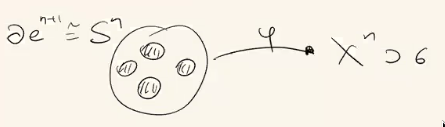
\includegraphics[width=0.8\linewidth]{shaded.png} \caption{Diagram
            of the morphism}% \label{fig:shaded} \end{figure} that the shaded
            part is $\varphi^{-1}(\sigma^n)$ and $\varphi$ is a homeomorphism
            on the shaded component. In particular, $f \circ \varphi, g \circ
            \varphi$ only differ on the shaded part, so the number of
            components of the shaded part is $[e:\sigma]$.  \end{proof}

\begin{proof}[Proof of fundamental theorem of obstruction theory] Let $\mc{O}_f
    = [c_f] = 0$. Then $c_f = \delta d$ for some $d \in \mc{C}^n(X, \pi_n(Y))$.
    But then there exists $g \colon X^n \to Y$ such that $\eval{g}_{X^{n-1}} =
    \eval{f}_{X^{n-1}}$ with $d_{f,g} = -d$. But then \[ c_g = c_f + \delta
    d_{f,g} = \delta d - \delta d = 0, \] so $g$ extends to $X^{n+1}$.

    In the other direction, assume $g \colon X^{n+1} \to Y$ with
    $\eval{g}_{X^{n-1}} = \eval{f}_{X^{n-1}}$. Therefore $c_g = 0$, and \[ c_f
    = c_f - c_g = - \delta d_{f,g}, \] so $[c_f] = 0$.  \end{proof}

Now we will consider the relative case. Suppose $(X, A)$ is a CW-pair and we
have $f \colon X^n \cup A \to Y$. Can we extend this to $X^{n+1} \cup A$? Here,
we obtain an obstruction class $\mc{O}_f \in H^{n+1}(X, A; \pi_n(Y))$. We have
a relative version of the fundamental theorem in this case.

Returning to the homotopy problem, consider $f, g \colon X \to Y$ such that
$\eval{f}_{X^{n-1}} \sim \eval{g}_{X^{n-1}}$. Can we extend this homotopy to
$X^n$? We are considering the extension problem for \[ X \times \qty{0} \cup
X^{n-1} \times I \cup X \times \qty{1} \subset X \times \qty{0} \cup X^n \times
I \cup X \times \qty{1}. \] We are considering $(n+1)$-cells of the form $e^n
\times I$, where $e^n$ is an $n$-cell in $X$. Assume for simplicity that
$\eval{f}_{X^{n-1}} = \eval{g}_{X^{n-1}}$. Then the obstruction is
\textbf{exactly} $d_{f,g} \in \mc{C}^n(X, \pi_n(Y))$. Also, if $c_f = c_g = 0$,
then $\delta d_{f,g} = c_g - c_f = 0$.

\begin{thm} Let $f, g \colon X \to Y$ agree on $X^{n-1}$. Then $H^n(X,
\pi_n(Y)) \ni [d_{f,g}] = 0$ if and only if $f,g$ are homotopic on $X^n$, with
the homotopy fixing $X^{n-2}$.  \end{thm}

\begin{exm}[Cohomology of $K(G, n)$] Consider $[X, K(G, n)] \to H^n(X, G)$ by
    $f \mapsto [d_{f, \text{const}}]$. Here, we can homotope $f$ such that
    $\eval{f}_{X^{n-1}}$ is constant because $\pi_i(K(G, n)) = 0$ for $i < n$.
    Surjectivity is obvious from the previous discussion, so we will prove
    injectivity.

    If $[d_{f, \text{const}}] = 0 \in H^n(X, G)$, then $\eval{f}_{X^n}$ is
nullhomotopic. Because $\pi_i(K(G, n)) = 0$ for $i > n$, $f$ is nullhomotopic.
\end{exm}

\section{Primary obstruction class}% \label{sec:primary_obstruction_class}

We will change our notation. Denote the fiber bundle by $F \hookrightarrow E
\to B$. In this new notation, we want to extend a section $s \colon B^n \to E$
to $B^{n+1}$. If $e^{n+1}$ is a cell, then $\eval{E}_{e^{n+1}} \cong e^{n+1}
\times F$. We have $s \colon \partial e^{n+1} \to F$ and we want to extend this
to $e^{n+1}$. Now we have the map $e^{n+1} \mapsto \mc{C}_s(e^{n+1}) \in
\pi_n(F)$. We know that $c_s \in \mc{C}^{n+1}(B, \pi_n(F))$. Now we know $s$
extends to $B^{n+1}$ if and only if $c_s = 0$, $\delta c_s = 0$, and the
obstruction class $\mc{O}_s \in H^{n+1}(B, \pi_n(F))$ is zero if and only if
$\eval{s}_{B^{n-1}}$ can be extended to $B^{n+1}$.

Now we assume that $F$ is $(n-1)$-connected. Therefore there exists a section
$s \colon B^n \to E$ with obstruction class $\mc{O}_s \in H^{n+1}(B,
\pi_n(F))$.

\begin{thm}\label{thm:obstA} Given $s, s' \colon B^n \to E$, we have $\mc{O}_s
= \mc{O}_{s'}$. In particular, this is an \textit{invariant} of the bundle!
\end{thm}

\begin{defn} Consider a fiber bundle $\xi \colon F \hookrightarrow E \to B$
with $F$ being $(n-1)$-connected. Then the \textit{primary obstruction class}
is defined by be $\mc{O}(\xi) \in H^{n+1}(B, \pi_n(F))$.  \end{defn}

\begin{thm} The fiber bundle $\xi$ always admits a section over $B^n$ and it
admits a section over $B^{n+1}$ if and only if $\mc{O}(\xi) = 0$.  \end{thm}

\begin{proof}[Proof of Theorem~\ref{thm:obstA}] First we note that a homotopy
    of $s$ does not change $C_s \in \mc{C}^{n+1}(B, \pi_n(F))$. The homotopy
    extension property holds for sections where $(X, A)$ is a CW pair with $s
    \colon X \to E$ and $s_t \colon A \times I \to E$ a homotopy of sections.
    Here, we can extend to $\wt{s}_t \colon X \times I \to E$.

    Now suppose $s, s' \colon B^n \to E$. Of course, $s \sim s'$ on $B^0$. We
now show that if $s \sim s'$ on $B^k$, then $s \sim s'$ on $B^{k+1}$ for $0
\leq k < n-1$. To see this, the homotopy extension property tells us that we
may assume $s = s'$ on $B^k$ after extending the homotopy. Then, we have
$d_{s,s'} \in \mc{C}^{k+1}(B, \pi_{k+1}(F))$. But we see that $d_{s,s'} = 0$,
so $s \sim s'$ on $B^{k+1}$. We now obtain $s, s' \colon B^n \to E$ such that
$s \sim s'$ on $B^{n-1}$. We may assume that $s = s'$ on $B^{n-1}$. Then we
note that $d_{ss'} \in \mc{C}^n(B, \pi_n(F))$, so $c_{s'} - c_s = \delta
d_{s,s'}$ and thus $\mc{O}_s = \mc{O}_{s'}$.  \end{proof}

The key property is that if we have $f \colon B' \to B$ and consider the
pullback bundle $f^* \xi$, then $\mc{O}(f^* \xi) = f^* \mc{O}(\xi)$. This tells
us that $\mc{O}(\xi)$ is a characteristic class, or in other words, a natural
cohomological invariant. Consider the basic example: Suppose $\xi \colon
S^{n-1} \hookrightarrow E \to B$ is an oriented bundle. Then $S^{n-1}$ is
$(n-2)$-connected, so we have an obstruction class $\mc{O}(\xi) \in H^n(B,
\Z)$.

\begin{defn} This obstruction class is called the \textit{Euler class} $e(\xi)$
of $\xi$. Then $e(\xi) = 0$ if and only if $\xi$ has a section over $B^n$.
\end{defn}

Here we have a special case. If $\eta \colon \R^n \hookrightarrow E \to B$ is
an oriented vector bundle and $\xi$ is the associated sphere bundle $S^{n-1}
\to S(E) \to B$. Then $e(E)$ is the Euler class of the associated sphere
bundle. Therefore $e(E) = 0$ if and only if there exists a nonvanishing section
of $\eta$ over $B^n$.

\begin{thm} Let $M^n$ be a smooth oriented compact manifold. Then $e(T_M) \in
H^n(M, \Z) \cong \Z$ is $\chi(M)$.  \end{thm}

\begin{cor}[Poincare-Hopf] $M$ admits a nowhere vanishing vector field if and
only if $\chi(M) = 0$.  \end{cor}

\begin{proof} Note that $M^{n-1} \cong M \setminus \qty{\text{finite number of
    points}}$ (one for each top-cell). To compute $\mc{O}(\xi)$ we can use a
    vector field $v$ with only isolated zeroes. Now we may define the local
    degree at $x$ to be the degree of the map $S_{\ep} \to S^{n-1}$ defined by
    $y \mapsto v(y)$. The local degree behaves like \begin{figure}[H]
        \centering 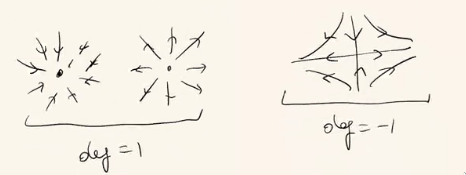
\includegraphics[width=0.8\linewidth]{locdeg}
        \caption{Example of local degrees}% \label{fig:locdeg} \end{figure} and
        therefore $\Z \ni \mc{O}(\xi) = \sum \text{local degrees}$ by
        definition. Now we simply need to construct an explicit nice vector
        field. Because $M$ is smooth, it admits a smooth
        triangulation.\footnote{Apparently there is also a proof using the
        Atiyah-Singer index theorem, but that is way more advanced than using
    this result. Francesco says this is a result everyone uses without knowing
the proof.} The vector field is constructed by placing a zero at the center of
every face and then for the center of a given positive dimensional face, the
vector field points outward towards the vertices of that face. But then we have
\[ \sum \text{local degrees} = \sum_i \#\qty{\text{$i$-cells}} = \chi(M).
\qedhere \] \end{proof}

\begin{rmk} Let $E^k \to M^n$ be a smooth vector bundle with $M$ compact. Then
    $e(E)$ can be interpreted as follows. Choose a generic section $s \colon M
    \to E$. Then $s^{-1}(0)$ is a smooth manifold of dimension $n-k$, and so we
    can write $e(E) = PD(s^{-1}(0))$.  \end{rmk}

We will now relate the primary obstruction class and transgression. We will
consider the Serre spectral sequence with coefficients in $\pi_n(F) = H_n(F)$.
We know we have the transgression map $\tau \colon H^n(F, \pi_n(F)) \to
H^{n+1}(B, \pi_n(F))$ and the fundamental class $\iota \in H^n(F, \pi_n(F))$.
This is defined by for all $x \in \pi_n(F), \ev{\iota, h(x)} = x$.

\begin{thm} The primary obstruction class is given by $\tau(\iota) =
\mc{O}(\xi) \in H^{n+1}(B, \pi_n(F))$.  \end{thm} Proof of this is given in a
series of exercises in Fuchs-Fomenko 23.5.

Now we will consider the \textit{Thom isomorphism}. If $E \to B$ is a rank $n$
vector bundle. Then we may associate the disk bundle $D(E)$ and the sphere
bundle $S(E)$. Now we define the \textit{Thom space} to be $T(E) = D(E) / S(E)$
(equivalently, the one-point compactification of $E$).

\begin{thm}[Thom isomorphism] Suppose $E$ is an oriented vector bundle. Then
    there exists a unique $U \in H^n(T(E); \Z) = H^n(D(E), S(E))$ such that
    $\eval{U}_{\ol{F}}$ is the generator of $H^n(\ol{F}, \Z) = \Z$ (given by
    orientation). We call $U$ the \textit{Thom class}. Furthermore, we have \[
        H^k(B, \Z) \cong H^k(D(E); \Z) \xrightarrow{\sim} H^{k+n}(D(E), S(E),
        \Z) \qquad x \mapsto x \cup U \] is an isomorphism for all $k$.
        Finally, the map \[ H^n(D(E), S(E)) \to H^n(D(E)) \cong H^n(B) \] sends
    the Thom class $U$ to the Euler class $e(E)$.  \end{thm}

\begin{proof} Consider the Serre spectral sequence for $(D^n, S^{n-1})
    \hookrightarrow (D(E), S(E)) \to B$. Then the Euler class is the Thom class
    by the prior discussion about transgression. Alternatively, we may
    construct the Thom class locally and patch, and this can be found in
    Chapter 10 of Milnor-Stasheff.  \end{proof}

\section{Vector Bundles}% \label{sec:vector_bundles}

We may consider the functor \[ \mr{Vect}_{\C}^k \colon \ms{CW}^{\mr{op}} \to
\ms{Set} \qquad X \mapsto \qty{\text{rank $k$ complex vector bundles}}. \] We
may also consider the functors $\Vect_{\R}^k, \Vect_{\R}^{+, k}$ of real vector
bundles and oriented real vector bundles. This functor is representable!

\begin{thm}[Brown representability] Let $h \colon \ms{hCW}_*^{\mr{op}} \to
    \ms{Set}$ be a functor. If \begin{enumerate} \item For $X = \bigvee
        X_{\alpha}$ with $i_{\alpha} \colon X_{\alpha} \hookrightarrow X$, then
        $\prod i_{\alpha}^* \colon h(X) \simeq \prod h(X_{\alpha})$ is an
        isomorphism; \item If $X = A \cup B$ is a union of subcomplexes and $a
\in h(A), b \in h(B)$ retrict to the same element in $h(A \cap B)$, then there
exists $x \in h(X)$ restricting to $a,b$, \end{enumerate} then there exists a
CW complex $K$ and $u \in h(k)$ such that \[ [X,k] \to h(X) \qquad f \mapsto
f^*(U) \] is a bijection.  \end{thm}

Note that for $\Vect_{\C}^k$, the condition of being homotopy invariant is
nontrivial to decide. We want $f_t \colon X \times I \to Y$ such that $f_0^*
\eta \simeq f_1^* \eta$. The idea is that for $\xi \coloneqq f_t^* \eta \to X
\times I$, we need $\eval{\xi}_{X \times 0} = f_0^* \eta, \eval{\xi}_{X \times
1} = f_1^* \eta$.

\begin{prop} Let $X$ be a CW complex (or in general $X$ is paracompact). Then
if $\xi$ is a vector bundle over $X \times I$, we have $\eval{\xi}_{X \times 0}
\simeq \eval{\xi}_{X \times 1}$.  \end{prop}

Recall that $X$ is \textit{paracompact} if $X$ is Hausdorff and any open cover
$\qty{U_{\alpha}}$ admits a locally finite refinement $\qty{V_{\beta}}$. This
is equivalent to every open cover admitting a partition of unity subordinate to
it.

\begin{rmk} We may also assume the indices $\beta$ are countable.  \end{rmk}

\begin{exm} Any $\eta \to X$ paracompact admits a Hermitian metric. To see
this, simply trivialize over the charts $U_{\alpha}$ and then glue using our
partition of unity.  \end{exm}

Now we note that if $E \to X \times [a,b]$ is trivial over $[a,c]$ and $[c,b]$,
then $E$ is trivial. This implies that any $\eta \to D^k$ is trivial. Fix
trivializations $h_1 \colon X \times [a,c] \times \C^k \to E_1$, $h_2 \colon X
\times [c,b] \times \C^k \to E_2$. These do not necessarily agree on $X \times
\qty{c} \times \C^k$, but we simply consider $\varphi = h_1 h_2^{-1}$ and
change $h_2$ by $\varphi$ to get the desired trivialization.

The second observation is that if $\eta \to X \times I$ then there exists an
open cover $\qty{U_{\alpha}}$ such that $\eval{\eta}_{U_{\alpha} \times I}$ is
trivial. To see this, we simply trivialize over $U_{X,i} \times [t_{i-1}, t_i]$
and then glue the trivializations.

Now we return to the proof that $\Vect_{\C}^k$ is homotopy invariant. Given a
partition of unity $\varphi_i$ subordinate to $U_{\alpha}$ (with
$\eval{eta}_{U_{\alpha} \times I}$ trivial), we write $\psi_m \colon \varphi_1
+ \cdots + \varphi_m \colon X \to [0,1]$. Then define $X_m$ to be the graph of
$\psi_m$. We know $\operatorname{supp} \varphi_{m+1} \subseteq U_{\alpha}$ for
some $\alpha$, so $p \colon X_{m+1} \to X_m$ lifts to $h_m \colon
\eval{\eta}_{X_{m+1}} \to \eval{\eta}_{X_m}$. We know $\eta$ is trivial on
$U_{\alpha} \times I$, so we have \[ h_m(x, \psi_{m+1}(x), v) = (x, \psi_m(x),
V). \] Then we know $X_0$ is $X \times \qty{0}$, so using local finiteness of
the partition of unity, we obtain the desired result.

We now want to find a concrete space that represents this functor. Define the
\textit{Grassmannian} \[ G_{n, k}^{\C} = \qty{k\text{-planes in }\C^n} \] of
$k$-planes in $\C^n$. This has a tautological bundle $\C^k \hookrightarrow
\gamma_{n, k}^{\C} \to G_{n,k}^{\C}$ given by $\gamma = \qty{(V, v) \mid v \in
V}$. Of course, if $m < n$, we know $G_{m,k}^{\C} \hookrightarrow
G_{n,k}^{\C}$, so we define $G_k^{\C} \coloneqq G_{\infty,k}^{\C} = \bigcup_n
G_{n,k}^{\C}$. Because the tautological bundles are well behaved under this, we
obtain a tautological bundle $\gamma_k \to G_k^{\C}$.

\begin{thm} The bundle $\gamma_k \to G_k^{\C}$ is a universal bundle. This
means that $[X, G_k^{\C}] \simeq \Vect_{\C}^k(X)$, where $f \mapsto f^*
\gamma_k$.  \end{thm}

\begin{rmk} We can also write $G_k^{\C} = BU(k)$ as the classifying space of
$U(k)$.  \end{rmk}

\begin{proof}[Proof of Theorem] Let $\eta \to X$. Then $\eta \cong f^*
    \gamma_k$ if and only if there exists $g \colon \eta \to \C^{\infty}$ which
    is linear injective on each fiber $\eta_x$. Given $p \colon \eta \to X$,
    choose a countable cover with $p^{-1}(U_i)$ trivial and $\varphi_i$ a
    partition of unity subordinate to $U_i$. Then define \[ g_i \colon
    p^{-1}(U_i) = U_i \times \C^n \to \C^n \] and consider the map $(\varphi_i
    \circ p) \cdot g_i \colon \eta \to \C^n$. This defines $g \colon \eta \to
    {(\C^n)}^{\infty} = \C^{\infty}$.

    Now we need to show that if $g_0, g_1 \colon \eta \to \C^{\infty}$ that are
    injective on fibers, then there exist $g_t \colon \eta \times I \to
    \C^{\infty}$ linear injective on fibers at each time. We define \[ L_t
    \colon \C^{\infty} \to \C^{\infty} \qquad (x_1, x_2, \ldots) \mapsto
(1-t)(x_1, x_2 \ldots) + t (x_1, 0, x_2, \ldots). \] This is injective at each
$t$ and moves $g_0$ to the odd entries. Similarly, we can move $g_1$ to the
even entries, so we can write $g_t = (1-t) g_0 + t g_1$.  \end{proof}

A \textit{characteristic class} is a natural transformation $\Vect_{\C}^k (X)
\xrightarrow{c} H^*(X, \Z)$. By the Yoneda lemma, characteristic classes are in
bijection with the cohomology of $G_k^{\C}$. We now study basic facts of the
Grassmannians: \begin{itemize} \item There is a transitive action of $U(n)$ on
    $G_{n,k}^{\C}$. The stabilizer of $\C^k \subset \C^n$ is $U(k) \times
    U(n-k)$.  \item Clearly we have $G_{n,1} = \C\P^{n-1}$.  \item The
    Grassmannian $G_{n,k}^{\C}$ has a nice cell decomposition generalizing
    $\C\P^n = \mr{pt} \cup D^2 \cup D^4 \cup D^6 \cup \cdots$.  \end{itemize}

\begin{exm} Consider the Grassmannian $G_{4,2}$ of $2$-planes in $\C^4$. Then
    the interior of cells is described by dimensions of intersections with
    $\C^1 \subset \C^2 \subset \C^4 \subset \C^4$. The cells are given by:
    \begin{description} \item[$0$-cell:] This is just $\qty{\C^2}$
        corresponding to $(1,2,2)$.  \item[$2$-cell:] This is the set
        $\qty{\C^1 \subset V \subset \C^3}$ corresponding to $(1,1,2)$.
    \item[$4$-cells:] These are $\qty{\C^1 \subset V}$ corresponding to
        $(1,1,1)$ and $\qty{V \subset \C^3}$ corresponding to $(0,1,2)$.
    \item[$6$-cell:] This is given by $\qty{\dim V \cap \C^2 > 0}$
        corresponding to $(0,1,1)$.  \item[$8$-cell:] This is everything else,
        which corresponds to $(0,0,1)$.  \end{description} \end{exm}

For an alternative description, a $2$ plane corresponds to the row reduced
echelon form of a $2 \times 4$ matrix. Then we have the following
correspondence: \begin{description} \item[$0$-cell:] This is the matrix $\mqty[
    0 & 0 & 1 & 0 \\ 0 & 0 & 0 & 1 ]$.  \item[$2$-cell:] This is the matrix
    $\mqty[ 0 & 1 & * & 0 \\ 0 & 0 & 0 & 1 ]$.  \item[$4$-cells:] These are the
    matrices $\mqty[ 1 & * & * & 0 \\ 0 & 0 & 0 & 1 ], \mqty[ 0 & 1 & 0 & * \\
    0 & 0 & 1 & * ]$.  \item[$6$-cell:] This is the matrix $\mqty[ 1 & * & 0 &
    * \\ 0 & 0 & 1 & * ]$.  \item[$8$-cell:] This is the matrix $\mqty[ 1 & 0 &
    * & * \\ 0 & 1 & * & * ]$.  \end{description} These cells are called
    \textit{Schubert cells}. These behave nicely with the inclusions and
    $G_{n,k}$ has $\binom{n}{k}$ cells. The number of $2i$-cells is given by
    the number of partitions of $i$ into at most $k$ integers that are each at
    most $n-k$. The cells are of even dimension, so we can compute the group
    structure on the cohomology, but not the ring structure.

\begin{thm} The ring struction on cohomology of the Grassmannian is given by
$H^*(G_k^{\C}, \Z) \cong \Z[c_1, \ldots, c_k]$, where $\deg c_i = 2i$.
\end{thm}

\begin{defn} The characteristic classes of $E \to B$ associated to the $c_i$
are the \textit{Chern classes} $c_i(E)$. By convention, $c_j(E) = 0$ for $j >
\dim E$.  \end{defn}

\begin{proof} We need many fibrations. Consider the spaces $G_{n,k}$ of
    $k$-planes in $\C^n$ and $F_{n,k}$ of $k$-flags in $\C^n$. It is clear that
    $F_{n,k}$ also parameterizes ordered $k$-tuples of orthogonal complex
    lines. Of course there is a fibration $F_{k, k} \hookrightarrow F_{n,k} \to
    G_{n,k}$. We can also understand $H^*(G_k^{\C})$ inductively as well.

    Now we will show that $H^*(F_{\infty,k}) \cong \Z[x_1, \ldots, x_k]$, where
    $\deg x_i = 2$. Each $x_i$ is the pullback of the generator of
    $H^2(\C\P^{\infty})$ under the maps $(\ell_1, \ldots, \ell_k) \mapsto
    \ell_i$. We will use the fibration $\C\P^{n-k} \hookrightarrow F_{n,k} \to
    F_{n,k-1}$. By induction, we have a fibration \[ \C\P^{\infty}
    \hookrightarrow F_{\infty, k} \to F_{\infty, k-1} \] and $H^*(F_{\infty},
    k-1) \cong \Z[x_1, \ldots, x_{k-1}]$. Now we use the Leray-Hirsch theorem,
    but first we need to show that $H^*(E) \twoheadrightarrow H^*(F)$. This is
    because we have the map $F_{\infty, k} \to \C\P^{\infty}$ given by
    $(\ell_1, \ldots, \ell_k) \to \ell_k$ and this restricts to the generator
    of $\C\P^{\infty}$ udner $\C\P^{\infty} \hookrightarrow F_{\infty, k}$.
    Therefore, $H^*(F_{\infty,k})$ is a free $\Z[x_1, \ldots, x_{k-1}]$-module
    with additive basis $1, x_k, x_k^2, \ldots$. Now we observe that \[
    F_{\infty, k} \hookrightarrow {(\C\P^{\infty})}^k \] is a homotopy
    equivalence by Hurewicz.

    Now we need to consider the fibration $F_{k,k} \hookrightarrow F_{\infty,
    k} \xrightarrow{\rho} G_{\infty, k}$. This induces a surjective map in
    cohomology, so by Leray-Hirsch, $H^*(F_{\infty}, k)$ is a free
    $H^*(G_{\infty}, k)$-module with basis $1, \ldots$ and thus $\rho^* \colon
    H^*(G_{\infty, k}) \to H^*(F_{\infty, k})$ is injective. The map
    $F_{\infty, k} \to G_{\infty, k}$ sends a $k$-tuple of lines to their sum.
    We also know that $\rho$ is $S_k$-invariant, so on cohomology, we have an
    injection \[ H^*(G_{\infty}, k) \hookrightarrow {H^*(F_{\infty,k})}^{S_k} =
    {\Z[x_1, \ldots, x_k]}^{S_k} = \Z[\sigma_1, \ldots, \sigma_k], \] where
$\sigma_i$ is the $i$th elementary symmetric polynomial. But then by a
dimension count, this injection is surjective.  \end{proof}

\begin{thm}[Splitting principle] Let $E^n \to X$ be a line bundle. Then there
exists $\wt{X} \xrightarrow{f} X$ such that $f^* E$ is a direct sum of line
bundles and $f^* \colon H^*(X, \Z) \to H^*(\wt{X}, \Z)$ is injective.
\end{thm} This gives us the following slogan: \begin{quotation} \textit{When
working with Chern classes, we can assume $E$ is a direct sum of line bundles
$E \cong L_1 \oplus \cdots \oplus L_k$.} \end{quotation}

\begin{proof} Set $\wt{X} = F_k(E) \to X$. Then the fiber over $x \in X$ is the
    space of $k$-flags in $E_x$. Therefore we have a fibration $F_{k,k}
    \hookrightarrow \wt{X} \to X$. Now $\wt{X}$ has a tautological splitting,
    where over the point $(\ell_1, \ldots, \ell_k)$ we have the vector space
    $\ell_1 \oplus \cdots \oplus \ell_k = E_x$. This pulls back $E$ as a direct
    sum of line bundles.  \end{proof}

Now here are some properties of Chern classes: \begin{enumerate} \item For any
    $E$, we have $c_0(E) = 1$.  \item If $\gamma$ is the tautological bundle
    over $\C\P^1$, then $c_1(\C\P^1) = -x$ and thus $\gamma = \mc{O}(-1)$.
\item For vector bundles $E, F$, we have $C_k(E \oplus F) = \sum c_k(E) \cup
    C_{k-i}(F)$. Equivalently, if we define the Chern class $c(E) = 1 + c_1(E)
    + c_2(E) + \cdots$, then $c(E \oplus F) = c(E) c(F)$.  \end{enumerate}

\begin{proof} We prove this for the universal bundles. We have the bundle
    $\gamma_k \times \gamma_{\ell}$ over $G_k \times G_{\ell}$, and this is
    given by a classifying map $G_k \times G_{\ell} \to G_{k + \ell}$. Now
    under the map ${(\C\P^{\infty})}^k \times {(\C\P^{\infty})}^{\ell} \to G_k
    \times G_{\ell}$, we know $\gamma_k \times \gamma_{\ell}$ pulls back to a
    direct sum of tautological bundles, and the same is true for
    $\gamma_{k+\ell}$ pulled back to ${(\C\P^{\infty})}^{k + \ell}$. Therefore,
    we have \[ c(\gamma_{k + \ell}) = (1 + x_1) \cdots (1 + x_k) (1 + y_1)
    \cdots (1 + y_{\ell}) = c(\gamma_k) c(\gamma_{\ell}). \qedhere \]
\end{proof}

In fact, the three properties determine the $\qty{c_i}$ uniquely.

\begin{rmk} \begin{itemize} \item If $\C$ is the trivial bundle, then $c_i(E
\oplus \C) = c_i(E)$.  \item If $\ol{E}$ is the complex conjugate bundle of
$E$, then $c_i(\ol{E}) = {(-1)}^i c_i(E)$. Note that this is also the dual
bundle.  \end{itemize} \end{rmk}

\begin{exm} We have $c(T \C\P^n) = {(1+x)}^{n+1} = 1 + nx + \binom{n}{2} x^2 +
    \cdots \in \Z[x]/x^{n+1}$. To describe this, we consider the tautological
    bundle $\gamma \to \C\P^{n+1}$. Clearly $T_L \C\P^n = \Hom_{\C}(L,
    L^{\perp})$, where the perp is taken in $\C^{n+1}$. Therefore, $T \C\P^n
    \equiv \Hom_{\C}(\gamma, \gamma^{\perp})$ and $\gamma \oplus \gamma^{\perp}
    = \C^{n+1}$. This gives us \begin{align*} T \C\P^n \oplus \C &\cong
        \Hom(\gamma, \gamma^{\perp}) \oplus \Hom(\gamma, \gamma) \\ &=
        \Hom(\gamma, \C^{n+1}) \\ &= {\Hom(\gamma, \C)}^{n+1} =
        {\mc{O}(1)}^{n+1} \end{align*} and therefore \[ c(T\C\P^n) = c(T\C\P^n
    \oplus \C) = {c(\mc{O}(1))}^{n+1} = {(1+x)}^{n+1}. \] \end{exm}

We will now consider Chern classes as obstructions. Let $\C^n \hookrightarrow E
\to B$ be a rank $n$ bundle. Then we can take orthonormal frames to obtain
$V_{n, k}^{\C} \hookrightarrow V_k(E) \to B$. Then sections of $V_k(E) \to B$
are $k$-tuples of sections of $E$ which are orthonomal at each point.

\begin{lem} We have \[ \pi_i(V_{n,k}^{\C}) = \begin{cases} 0 & i \leq 2 (n-k)
\\ \Z & i = 2(n-k) + 1.  \end{cases} \] \end{lem}

Therefore, the first obstruction to finding a section of $V_k(E)$ over the
$2(n-k) + 2$ skeleton lives in $H^{2(n-k)+2}(B, \Z)$. In fact, this is the
Chern class. The Chern class $c_j(E) \in H^{2j}(B, \Z)$ is the obstruction to
finding $k = (n+1-j)$ linearly independent sections over the
$2(n+1-j)$-skeleton. Now observe that $V_{n,1} = S^{2n-1}$. Therefore, if
$\dim_{\C} E = n$, we have $c_n(E) = e(E)$.

\section{Real Vector Bundles}% \label{sec:real_vector_bundles}

Now consider a vector bundle $\R^n \hookrightarrow E \to B$.

\begin{lem} For $i < n-k$, we have $\pi_n(V_{n,k}^{\R}) = 0$. In addition, \[
    \pi_{n-k}(V_{n,k}^{\R}) = \begin{cases} \Z & k=1 \text{ or } n-k \text{
    even. } \\ \Z_2 & \text{otherwise}.  \end{cases} \] \end{lem} Therefore we
    obtain obstruction classes $\mc{O}_i \in H^i(B, \wt{Z})$ or $\mc{O}_i \in
    H^i(B, \Z_2)$. This is an obstruction to finding $n+1-i$ linearly
    independent sections on the $i$-skeleton. Reducing everything modulo $2$,
    we have \begin{defn} The \textit{Stiefel-Whitney classes} of $E$ are
        defined by $w_i \coloneqq \mc{O}_i \mod 2$.  \end{defn} Here are some
        facts about the Stiefel-Whitney classes: \begin{itemize} \item If
            $\gamma \to \R\P^1$ is the tautological class, then $w_1(\gamma) =
            1 \in H^1(\R\P^1, \Z_2)$.  \item These correspond to $H^*(G_k^{\R};
            \Z_2) = \Z_2[w_1, \ldots, w_k]$, where $\abs{w_i} = i$. Note that
            it is harder to compute the cohomology in this case than in the
            complex case.  \item We have $w_1(E) = 0$ if and only if $E$ is
            orientable.  \item If $\dim E = n$ and $E$ is orientable, then
    $w_n(E) = e(E) \mod 2$.  \item They are related to $\Sq^{\bullet}$ on
    $T(E)$ (and in fact this is the definition given in Milnor-Stasheff).
    \end{itemize}

Now we will assume that our real vector bundles are oriented. Recall that
$G_k^{\R} = BO(k)$ is the space of $k$-planes in $\R^{\infty}$. Then we set
$G_k^+ = BSO(k)$ to be the space of \textbf{oriented} $k$-planes in
$\R^{\infty}$. There is a double cover $G_k^+ \to G_k^{\R}$. Recall that every
oriented bundle has an Euler class!  \begin{rmk} Suppose $E \to B$ is an
oriented odd-dimensional vector undle. Then the map $(b, v) \mapsto (b,-v)$
reverses orientation on the sphere bundle, so $e(E) = -e(E)$ and thus $2e(E) =
0$.  \end{rmk}

Recall that $H^*(SO(n), \Q)$ varies greatly depending on the parity of $n$. We
should obtain the same thing for the classifying spaces.

\begin{thm} Over $\Q$, we have $H^*(G_{2m+1}^+) \Q[p_1, \ldots, p_m]$, where
$\abs{p_i} = 4i$. In the even case, we have $H^*(G_{2m}^+) = \Q[p_1, \ldots,
p_m, e]/(e^2=p_m)$.  \end{thm} We are mostly interested in even-dimensional
manifolds, so we will mostly work in the second case.

\begin{defn} The characteristic classes corresponding to $p_1, \ldots, p_m$ are
called the \textit{Pontryagin classes} of $E$.  \end{defn}

Concretely, we can define the Pontryagin classes in terms of the Chern classes.
If $E \to B$ is a real vector bundle, we may take $E \otimes \C \to B$ the
corresponding complex vector bundle. Then we have \[ p_i(E) \coloneqq {(-1)}^i
c_{2i}(E \otimes \C) \in H^{4i}(B, \Z). \]

\begin{rmk} Recall that $E \otimes \C$ is always isomorphic to its dual.
Complex conjugation gives an antilinear involution, so $c_{2i+1}$ is
$2$-torsion.  \end{rmk}

\begin{exm} We will compute the Pontryagin classes of $T\C\P^n$.  \end{exm}

\begin{lem} If $E$ is already a complex vector bundle, then $E \otimes \C \cong
E \oplus E^*$ as complex vector bundles.  \end{lem}

\begin{proof} Define by $i$ the complex structure on $E$. Then the map $(v,0)
\mapsto (v,-iv), (0,w) \mapsto (w,iw)$ is a $\C$-linear isomorphism.
\end{proof}

In particular, if $E$ is complex, then the \textit{total Pontryagin class}
$p(E) = 1 + p_1(E) + p_2(E) + \cdots$ can be computed using \begin{align*} 1 -
    p_1(E) + p_2(E) - p_3(E) + \cdots &= 1 + c_2(E \otimes \C) + c_4(E \otimes
    \C) + c_6(E \otimes \C) \\ &= c(E \otimes \C) \\ &= c(E \oplus E^*) \\ &=
    c(E) \cdot c(E^*) \\ &= (1 + c_1(E) + c_2(E) + \cdots) (1-c_1(E) + c_2(E) -
    c_3(E) + \cdots).  \end{align*} For $T\C\P^n$, we have \begin{align*} 1 -
    p_1 + p_2 - p_3 + \cdots &= {(1+x)}^{n+1} {(1-x)}^{n+1} \\ &=
    {(1-x^2)}^{n+1}, \end{align*} so we obtain \[ p_k(\C\P^n) = \binom{n+1}{k}
a^{2k}. \]

Now we will consider Pontryagin roots. The splitting principle for $E^{2m} \to
B$ says that $E$ can always be thought of as a direct sum of oriented $2$-plane
bundles analogously to Chern classes. Note that an oriented $2$-plane bundle is
the same as a complex line bundle (because $i$ rotates by $\frac{\pi}{2}$
counterclockwise). In the case where we actually have $E = L_1 \oplus L_2
\oplus \cdots \oplus L_n$, we obtain \[ E \otimes \C = L_1 \oplus L_1^* \oplus
L_2 \oplus L_2^* \oplus \cdots \oplus L_m \oplus L_m^*. \] These have Chern
roots $\pm x_1, \pm x_2, \ldots, \pm x_m$, so we have \begin{align*} p_1(E) &=
    -c_2(E \otimes \C) = x_1^2 + x_2^2 + \cdots + x_m^2 \\ p_2(E) &=
    \sigma_2(x_1^2, \ldots, x_m^2) \\ \vdots & \\ p_m(E) &= x_1^2 x_2^2 \cdots
x_m^2 = \sigma_m(x_1^2, \ldots, x_m^2).  \end{align*} This tells us that the
$x_i^2$ are the Pontryagin roots. Also, $e(E) = x_1 \cdots x_m$, so $e^2 =
p_m$.

\begin{rmk} This is related to the fact that $\det \colon \mf{so}(2m) \to \R$
has an $SO(2m)$-invariant square root, called the \textit{Pfaffian}.  \end{rmk}

\subsection{Relation to Steenrod problem and oriented bordism}%
\label{sub:relation_to_steenrod_problem_and_oriented_bordism}

Let $X^n$ be a closed smooth manifold and $\alpha \in H_k(X, \Z)$.
\begin{quest} Is there an oriented smooth manifold $M^k$ and continuous $f
\colon M \to X$ such that $f_*[M] = \alpha$?  \end{quest}

\begin{defn} A pair $(M, f)$ is \textit{singular manifold} representing
$\alpha$.  \end{defn}

Now define \[ \Omega_k(X) \coloneqq \frac{ \qty{(M^k, f)\ \text{singular
manifold in $X$}} }{\qty{(M, f) \mid \text{there exists }\partial W = M, f\
\text{extends to $W$}}} \] with addition given by disjoint union. In addition,
we set $-[M, f] = [\ol{M}, f]$. This is well-defined, and in fact there is a
map \[ \Omega_n(X) \to H_n(X, \Z) \qquad [(M, f)] \mapsto f_*[M]. \] The group
$\Omega_k(X)$ is called the $k$-th \textit{bordism group}. Clearly $\Omega_k$
is functorial by postcomposition.

\begin{rmk} The functors $\Omega_*$ give a generalized homology theory. Note
    that $\Omega_k(\mr{pt})$ is very complicated. These are given by \[
    \Omega_k(\mr{pt}) = \frac{\qty{M^k \text{ oriented $k$-manifolds}}}{\qty{M
= \partial W^{k+1}}}. \] \end{rmk}

\begin{thm} If $M^{4k} = \partial W^{4k+1}$, then the signature of $M$ is $0$.
\end{thm}

\begin{exm} In $\Omega_{4k}(\mr{pt})$, $[\C\P^{2k}] \neq 0$.  \end{exm}

\begin{lem} If $B \colon V \otimes V \to \R$ is symmetric and nondegenerate and
$W \subset V$ is isotropic and $\dim W = \frac{1}{2} \dim V$, then the
signature of $B$ is $0$.  \end{lem}

\begin{rmk} Actually, it is easy to see that $B = \begin{psmallmatrix} 0 & W \\
1 & 0 \end{psmallmatrix}^{\oplus \dim W}$.  \end{rmk}

\begin{lem} Let $\iota \colon M \hookrightarrow W$ be the inclusion onto the
boundary. Then $\ev{\iota^*(c), [M]} = 0$ for all $c \in H^{4k}(W)$.  \end{lem}

\begin{proof} This is given by $\ev{i^*(c), [M]} = \ev{c, i_* [M]} = 0$ because
    in the exact sequence \[ H_{4k+1}(W, M) \xrightarrow{\delta} H_{4k}(M)
    \xrightarrow{\iota_*} H_{4k}(W),\] we have $[W.M] \mapsto [M]$, so $[M] =
0$.  \end{proof}

\begin{proof}[Proof of Theorem] Consider the commutative diagram
    \begin{equation*} \begin{tikzcd} H^{2k}(W) \ar{r}{\iota^*} \ar[equal]{d} &
        H^{2k}(M) \ar[equal]{d} \ar{r} & H^{2k+1}(W, M) \ar[equal]{d} \\
        H_{2k+1}(W, M) \ar{r} & H_{2k}(M) \ar{r}{\iota_*} & H_{2k}(W).
    \end{tikzcd} \end{equation*} We know that $W = \Im(\iota^* \colon H^{2k}(W)
    \to H^{2k}(M))$ is isotropic in $V = H^{2k}(M)$, so we need to show that it
    is half-dimensional. But then $\Im(\iota^*) = \ker (\iota_*)$ under
    identification. But then $\iota^*$ is dual to $\iota_*$, so $\dim
    \Im(\iota^*) = \dim \Im(\iota_*) = \dim V - \dim \ker (\iota_*)$ and thus
    $W$ is half-dimensional.  \end{proof}

Recall that a \textit{spectrum} $\mathbb{E}$ is a sequence $(E_n, j_n \colon
\Sigma E_n \to E_{n+1})$. Then we have the associated homology theory \[ H_n(X,
\mathbb{E}) = \varinjlim \pi_{n+\ell} (X_+ \wedge E_{\ell}), \] where the
colimit is over the sequence of maps given by suspension followed by
$j_{\ell}$.

\begin{exm} Consider $E_n = K(\Z, n)$ and let $j_n$ be adjoint to $\Omega K(\Z,
n+1) = K(\Z, n)$. Then the associated homology theory is $H_n(-, \Z)$.
\end{exm}

Thom described the spectrum representing $\Omega_n$. Nowadays we call this the
\textit{Thom spectrum} $MSO$. Here, we write $MSO(k) = T(\gamma_k \to BSO(k))$,
where $BSO(k)$ is the oriented Grassmannian. Then there is a natural map \[
\iota_k \colon BSO(k) \to BSO(k+1) \qquad \R^{\infty} \supset V \mapsto \R
\oplus V \in \R \oplus \R^{\infty} = \R^{\infty}. \] In particular, we have
$\iota_k^* \gamma_{k+1} = \underline{\R} \oplus \gamma_k$. Then we have a map
$T(\R \oplus \gamma_k) \to T(\gamma_{k+1})$, but in the homework we prove that
$T(\R \oplus E) = \Sigma T(E)$.

\begin{thm}[Thom 1954] The spectrum $MSO$ represents the homology theory
$\Omega_*$.  \end{thm}

As a consequence, we have $\Omega_n(\mr{pt}) = \varinjlim
\pi_{n+\ell}(MSO(\ell))$. In particular, this is finitely generated. Tensoring
with $\Q$, we may use techniques of Serre to prove that \[ \Omega_n(\mr{pt})
\otimes \Q = \varinjlim H_{n+\ell} (MSO(\ell), \Q) = \varinjlim_{\ell \to
\infty} H_n(BSO(\ell), \Q). \] Therefore $\Omega_n(\mr{pt})$ is finitely
generated with rank $0$ when $4 \nmid n$ and the number of partitions of $i$
when $n = 4i$.

\begin{rmk} The generators of $\Omega_{4i}(\mr{pt}) \otimes \Q$ are
    $\C\P^{2i_1} \times \cdots \times \C\P^{2i_k}$, where $I = (i_1, \ldots,
    i_k)$ is a partition of $i$. Alternatively, we may define \[ p_I \colon
    \Omega_{4i} (\mr{pt}) \to \Z \qquad M \mapsto \ev{p_{i_1}(M) \cup \cdots
\cdots p_{i_j}(M), [M]}. \] This is called the \textit{$I$-Pontryagin number}.
Then the map \[ \Omega^{4i}(\mr{pt}) \to \Z^{\# \text{partitions}} \qquad M
\mapsto \qty{p_I(M)} \] is an isomorphism after tensoring with $\Q$. 

    Recall that the signature gives a homomorphism $\Omega_{4i}(\mr{pt}) \to
    \Z$. Therefore it is a linear combination of Pontryagin numbers. We may
    compute exactly which combination using the \textbf{Hirzebruch signature
    theorem}. Later, we will prove this as a consequence of the Atiyah-Singer
    index theorem. We have \begin{enumerate} \item $\mr{sign}(M^4) =
        \frac{1}{3} p_1$.  \item $\mr{sign}(M^8) = \frac{1}{45} (7p_2 -
        p_1^2)$.  \item $\mr{sign}(M^{12}) = \frac{1}{945}(62p_3 - 13 p_1p_2 +
        2 p_1^3)$.  \item $\mr{sign}(M^{16}) = \frac{1}{14175}(\ldots)$.
    \end{enumerate} \end{rmk} An application of this formula is in Milnor's
    1956 paper \textit{On manifolds homeomorphic to the $7$-sphere}.
    \begin{thm}[Milnor 1956] There exist $M^7$ which are homeomorphic but not
        diffeomorphic to $S^7$.  \end{thm} The idea to distinguish smooth
        structures is this. We know $H^*(M^7, \Z) \cong H_*(S^7, \Z)$. Then
        because $\Omega_7 = 0$ there exists $W^8$ such that $M^7 = \partial
        W^8$. Then we have an intersection form on $H^4(W, M,
        \Z)/\text{torsion} \cong H^4(W)/\text{torsion}$. In particular, the
        signature of $W$ is an integer and have a number $q(W) = \ev{p_1^2(W),
        [W,M]}$.  \begin{lem} The number $\lambda = 2q(W) - \text{sign}(W) \mod
        7$ is is independent of the choice of $W$. Therefore $\lambda$ is an
    invariant of $M$.  \end{lem}

\begin{proof} Consider two bounding manifolds $W_1, W_2$. Then we can glue
    $W_1, W_2$ to obtain a closed manifold $X$. Then $\sign(X) = \sign(W_1) -
    \sign(W_2)$ and $\ev{p_1^2(X), [X]} = q(W_1) - q(W_2)$. Then the Hirzebruch
    formla gives us \[ 45 \sign + p_1^2 = 7 p_2 \] and now basic arithmetic
gives us the desired result.  \end{proof}

\begin{rmk} This is a diffeomorphism invariant of $M$. Then $\lambda(S^7) = 0$
because $S^7$ bounds $S^8$ and gluing them together gives $S^8$.  \end{rmk}

\begin{exms} We will give examples of $M^7$ homeomorphic to $S^7$ but not
    diffeomorphic to it. We will construct these as sphere bundles of oriented
    rank $4$ bundles over $S^4$. Consider $\R^4 \hookrightarrow E \to S^4$.
    These can be described using \textit{clutching functions}. If we take $S^4
    = D_+^4 \cup D_-^4$, and we know $\eval{E}_{D_{\pm}} = D_I \times \R^4$.
    Therefore it suffices to describe the gluing along the equator, which gives
    us a map $S^3 \to SO(4)$. Now oriented vector bundles are described by
    $\pi_3(SO(4)) = \Z \oplus \Z$. 

    Very explicitly, we can identify $S^4$ with the unit quaternions and $\R^4
    = \H$. Then $f_{gj} \colon S^3 \to SO(4)$ is defined by \[ f_{hj}(u) \cdot
    x = u^h x u^j. \] For example, the trivial map $f_{0,0}$ is given by $S^4
    \times \R^4$. The unit sphere is $S^4 \times S^3$. Similarly, $f_{1,0}$
    gives $\gamma \to \H\P^1$ and gives us the unit sphere $S^7$. Now for $k$
    odd, we will choose $h,j$ such that $h+j=1, h-j=k$. Then define $M_k$ to be
    the unit sphere bundle for $f_{hj}$.

    We will see that $M_k$ is homeomorphic to $S^7$ but $\lambda(M_k) = k^2-1$.
Thus $M_3$ is homeomorphic but not diffeomorphic to $S^7$. First, we will write
an explicit $f \colon M_k \to \R$ with exactly one maximum and minimum. Then
using gradient flow, we have $M_k = D^7 \cup_{\varphi} D^7$ via some $\varphi
\colon \partial D^7 \to \partial D^7$. Because $\varphi$ extends radially to
$D^7$, we have a homeomorphism $M_k \cong S^7$. To compute $\lambda(M_k)$, note
that $M^7$ bounds the unit disk bundle of $E \to S^4$.  \end{exms}

\section{Topological K-theory}% \label{sec:topological_k_theory}

Let $X$ be a \textbf{finite} CW complex (more generally a compact Hausdorff
space). Then let $\Vect(X)$ denote the set of isomorphism classes of (complex)
vector bundles on $X$.

\begin{rmk} The rank may vary on each component of $X$.  \end{rmk}

Then $\Vect(X)$ is a unital semiring with operations $\oplus, \otimes$ and unit
the trivial line bundle $\underline{\C}$.

\begin{rmk} Unlike $\N$, $\Vect(X)$ is \textbf{not} cancellative. This means
that if $a+b = c+b$, then $a \neq c$ in general.  \end{rmk}

\begin{exm} Consider $TS^2 \oplus \ul{\R} = \ul{\R^3}$. However, $TS^2 \neq
\R^2$.  \end{exm}

We may define $\Z = \qty{(a,b) \in \N^2} / (a+b' = a'+b)$. This only works
because $\N$ is cancellative, but if we modify the condition to be $(a,b) \sim
(a',b')$ if $a+b'+e = a'+b+e$ for some $e$, then this defines the
\textit{Grothendieck ring}.

\begin{defn} Define the \textit{K-theory ring} $K(X)$ to be the Grothendieck
ring of $\Vect(X)$.  \end{defn}

This defines a functor from $\ms{finCW}^{\mr{op}} \to \ms{Ring}$.

\begin{exm} We know that $\Vect(\mr{pt}) = \N$, so $K(\mr{pt}) = \Z$. This is
because vector bundles on a point are the same as vector spaces.  \end{exm}

Thus if we consider the inclusion $\mr{pt} \hookrightarrow X$, we obtain the
(virtual) rank map $K(X) \to K(\mr{pt}) = \Z$. This is locally constant. Note
that if $X$ is finite, then given $E \to X$, there is $E' \to X$ such that $E
\oplus E' \cong \ul{\C}^n$ for some $n$. Here are some consequences:
\begin{enumerate} \item If $\alpha \in K(X)$, then we can write $\alpha = a -
    \C^N$ for some $a, N$. Here, if $\alpha = E-F$, then we choose $F \oplus F'
    \cong \C^N$, and thus we get $\alpha = E + F' - \C^N$.  \item If $\alpha =
    a + \C^N$ and $\beta = b - \C^M$, then $\alpha = \beta$ if and only if they
    have the same rank everywhere and $a,b$ are stably equivalent (which means
    that $a \oplus \C^A = b + \C^B$ for some $A,B$).

        To see this, we have $a + \C^M + \mc{E} = b + \C^N + \mc{E}$ for some
$\mc{E}$. Then we simply add $\mc{E}'$ such that $\mc{E} + \mc{E}' = \C^L$. Now
we have $a + \C^{M+L} = b + \C^{N+L}$, so we are done.  \end{enumerate}

Now we would like to throw away the information about stably equivalent
bundles. If $(X, x_0)$ is a pointed space, we define the \textit{reduced
K-theory} $\wt{K}(X, x_0) \coloneqq \ker (K(X) \to K(x_0)) = \Z$. This depends
only on the component of $x_0$ and is a non-unital ring. 

\begin{prop} We can identify $\wt{K}(X, x_0)$ with vector bundles on $X$ up to
stable equivalence.  \end{prop}

Now stabilization corresponds to the inclusion $BU(k) \hookrightarrow BU(k+1)$,
so a bundle up to stabilization has classifying space $BU \coloneqq BU(\infty)
= \bigcup BU(k)$. Therefore, we have

\begin{cor} $\wt{K}(X) = [X, BU]$.  \end{cor}

\begin{rmk} This is false for noncompact spaces in general.  \end{rmk}

We may also take the maps \[ U(k) \hookrightarrow U(k+1) \qquad A \mapsto
\mqty(1 & 0 \\ 0 & A). \] Now we define $U \coloneqq U(\infty) = \bigcup_k
U(k)$. Then we have a fibration $U \hookrightarrow EU \to BU$, where $EU =
V^{\C}(\infty, \infty)$. We also have fibrations \[ U(K) \hookrightarrow
V_{\C}(\infty, k) \to BU(k). \] Because $\pi_r(V_{\C}(n, k)) = 0$ for $r \leq
2(n-k)$, we see that $V_{\C}(\infty, \infty)$ is contractible.

\begin{exm} It is easy to see that \[ \wh{K}(S^1) = [S^1, BU] = \pi_1(BU) =
    \pi_0(U) = 0. \] Similarly, we have \[ \wt{K}(S^2) = [S^2, BU] = \pi_2(BU)
= \pi_1(U) = \pi_1(U(1)) = \Z. \] If $\gamma$ is the tautological class (here,
take $S^2 = \C\P^1$), then this is generated by $\gamma - 1$. This is because
$c_1(\gamma) = -1$. Therefore $K(S^2) = \wt{K}(S^2) \oplus \Z = \Z \oplus \Z$
is generated by $\gamma, 1$. The map is given by $a \mapsto (c_1(a), \dim(a))$.
Now that $(\gamma \otimes \gamma) \oplus 1 \cong \gamma \oplus \gamma$. In
particular, ${(\gamma-1)}^2 = 0$. Thus we have $K(S^2) \cong \Z[\gamma]/{
(\gamma-1) }^2$.  \end{exm}

Now we would like to extend this to a generalized cohomology theory.

\begin{lem} Let $(X, A)$ be a finite CW pair. Then $\wt{K}(X/A) \to \wt{K}(X)
\to \wt{K}(A)$ is exact (because $A \subset X$ is a cofibration).  \end{lem}

Because $A \subset X$ is a cofibration, we know that $X/A \simeq X \cup CA$.
Now the exact sequence extends to \[ A \hookrightarrow X \to X/A \to \Sigma A
\to \Sigma X \to \Sigma X/A \to \cdots \] by our discussion of cofiber
sequences from last semester. This gives us a long exact sequence \[ \cdots \to
\wt{K}(\Sigma X/A) \to \wt{K}(\Sigma X) \to \wt{K}(\Sigma A) \to \wt{K}(X/A)
\to \wt{K}(X) \to \wt{K}(A). \] Now we can manually define a cohomology theory
as follows: \begin{defn} For $q > 0$, define $\wt{K}^{-q}(X) \coloneqq
    \wt{K}(\Sigma^q X)$. Analogously there is an unreduced theory $K^{-q}(X,A)
    = \wt{K}(\Sigma^q(X/A))$. This gives $K^{-q}(X) \coloneqq K^{-q}(X,
    \emptyset) = \wt{K}(\Sigma^q(X \sqcup \mr{pt}))$.  \end{defn}

\begin{exm} We have $K^{-q}(\mr{pt}) = \wt{K}(\Sigma^q(S^0)) = \wt{K}(S^q) =
\pi_q(BU)$.  \end{exm}

The K-groups satisfy a miraculous identity: \begin{thm}[Bott periodicity,
version B] For all spaces $X$, $\wt{K}(\Sigma^2 X) \cong \wt{K}(X)$.  \end{thm}
Therefore $K^{-q}$ is $2$-periodic and we will consider $K^0, K^1$ as the
interesting cases. The original statement of Bott periodicity is

\begin{thm}[Bott periodicity, version C] The homotopy groups $\wt{K}(S^q) =
\pi_q(BU) = \pi_{q-1}(U)$ are $2$-periodic. Therefore $\pi_k(U) = \Z$ is $k$ is
odd and $0$ if $k$ is even.  \end{thm}

The most useful form of this result is \begin{thm}[Bott periodicity, version A]
    For all spaces $X$, we have $K(X \times S^2) =
    K(X)[\gamma]/{(\gamma-1)}^2$. Here, $\gamma$ is the pullback of the
    tautological bundle $\gamma \to \C\P^1 = S^2$.  \end{thm}

Concretely, we have a map \[ K(X) \oplus K(X) \xrightarrow{\sim} K(X \times
S^2) \qquad (\alpha_1, \alpha_2) \mapsto (\alpha_1 \otimes \C) \oplus (\alpha_2
\otimes \gamma). \] Francesco says that proving this result is difficult
online, so we only give a sketch.

\begin{proof}[Sketch of proof] We will use generalized clutching functions.
    Choose a bundle $E \to X$. This gives a bundle $E \to X \times D^2_{\pm}$.
    But of course $D^2$ is contractible, so we can glue them together using
    some $f \colon X \times S^1 \to \Aut(E)$. Thus $f(x,z) \in GL(E_{(x,z)})$,
    so we obtain a class $[E, f]$.

    The key point is that stably, any bundle on $X \times S^2$ has the form
$[E,1] \oplus [E', z]$.  \end{proof}

\begin{exm} We can represent $\gamma \to S^2$ as $[\mr{pt}, f(x,z) = z]$.
\end{exm}

\begin{proof}[Proof of version B] Consider the long exact sequence \[ \cdots
\to K^{-1}(X \times S^2) \xrightarrow{\varphi_{-1}} K^{-1}(X \vee S^2) \to K(X
\times S^2, X \vee S^2) \to K(X \times S^2) \xrightarrow{\varphi} K(X \vee S^2)
\to \cdots \] Therefore $\varphi$ is surjective because $K(X \vee S^2) =
\wt{K}(X \vee S^2) \oplus \Z = \wt{K}(X) \oplus \wt{K}(S^2) \oplus \Z$. This
argument also works for $\varphi_{-1}$, and thus \[ \wt{K}(\Sigma^2 X) = \ker
(K(X \times S^2) \xrightarrow{\varphi} K(X \vee S^2)). \] By version A, we see
that $x = \alpha_1 \otimes \C + \alpha_2 \otimes \gamma = \alpha \otimes
(\gamma-1) + \beta \otimes \gamma$. If if $x \in \ker \varphi$, , then its
restrictions to both $X, S^2$ are trivial. Restricting to $X$, we require that
$0 = \alpha \dim(\gamma-1) + \beta \dim \gamma = \beta$. Restricting to $S^2$,
we see that $0 = \dim \alpha \cdot (\gamma-1)$, so $\alpha \in \wt{K}(X)$.
Therefore the map $\wt{K}(X) \to \wt{K}(\Sigma^2 X)$ given by $\alpha \mapsto
\alpha \otimes (\gamma-1)$ is an isomorphism.  \end{proof}

\begin{cor} The group $\wt{K}(S^{2n}) = \Z$ is generated by
${(\gamma-1)}^{\otimes n}$ and $\wt{K}(S^{2n+1}) = 0$.  \end{cor}

Now we want to consider $\wt{K}(X)$ in the noncompact case. The options are
\begin{enumerate} \item The Grothendieck ring of $\Vect(X)$; \item The set of
maps $[X, BU]$; \item The limit $\varprojlim K(Y)$ for compact $Y$.
\end{enumerate}

Unfortunately these are not the same. We are interested in the case where $X$
is Hausdorff and locally compact. For example, if $X$ is a CW complex such that
every point is contained in only finitely many cells or if $E \to X$ is a
vector bundle to a compact Hausdorff space, then $E$ is Hausdorff and locally
compact. In our case, the one-point-compactification $X^+$ is Hausdorff.

\begin{defn} If $X$ is locally compact and Hausdorff, define $K(X) \coloneqq
\wt{K}(X^+, \infty)$.  \end{defn}

This is a (unital) ring and is functorial under proper maps. Also, if $U
\subset X$ is open and relatively compact with $U^+ = X / X \setminus U = X^+ /
X^+ \setminus U$, we obtain a map $X^+ \to U^+$. In particular, we obtain a map
$K(U) \to K(X)$. Then we have \[ K(X) = \varinjlim K(U), \] where $U$ ranges
over the relatively compact subsets of $X$. Of course, if $X$ is compact, we
recover the original $K$-theory.

There is an alternative point of view in terms of complexes. Let \[ 0 \to E_0
\to E_1 \to \cdots \to E_n \to 0 \] be a complex of bundles over $X$. We define
the \textit{support} $\supp \mathbb{E}$ to be the locus where the sequence is
not exact.

\begin{exm} If we consider the bundle $0 \to \C \xrightarrow{z} \C \to 0$, then
the support of this complex is $\qty{0}$.  \end{exm}

Define $C(X)$ to be the homotopy classes of complexes with compact support,
where $\E_0 \sim E_1$ if there exists $\mathbb{G} \to X \times I$ with compact
support and $\eval{\mathbb{G}}_{X \times \qty{i}} = \E_i$. Now this contains
the set $C_{\emptyset}(X)$ of complexes with empty support. 

\begin{prop}[Segal] If $X$ is Hausdorff and locally compact, then $K(X) \cong
C(X) / C_{\phi}(X)$ as rings.  \end{prop}

The basic idea is that if $E - F \in K(X) = \wt{K}(X, \infty)$, then the
dimensions of $E, F$ are equal at $\infty$, so we can consider the complex $0
\to E \xrightarrow{\alpha} F \to 0$ where $\alpha$ is a chosen isomorphism near
$\infty$ and extended arbitrarily with compact support to the entire $X$.

\begin{rmk} We have the inclusion $\supp(\E \otimes \E') \subseteq \supp(\E)
\cap \supp(E')$. Therefore, the multiplication is well-defined.  \end{rmk}

\begin{rmk} The sequence $0 \to \C \xrightarrow{z} \C \to 0$ in $K(\R^2) =
\wt{K}(S^2)$ corresponds to $\gamma - 1$.  \end{rmk}

\begin{exm} We have $K(\R^{2n}) = \wt{K}(S^{2n}) = \Z$ and this is generated by
    ${(\gamma-1)}^{\otimes n}$. The idea is to tensor multiple copies of $0 \to
    \C \xrightarrow{z_i} \C \to 0$, and the generator is the \textit{Koszul
    complex} \[ 0 \to {\bigwedge}^0 \C^n \xrightarrow{\wedge \zeta}
    {\bigwedge}^1 \C^n \xrightarrow{\wedge \zeta} {\bigwedge}^2 \C^n \to \cdots
\to {\bigwedge}^n \C^n \to 0. \] \end{exm}

Now recall the Thom isomorphism in cohomology. If $\R^n \hookrightarrow E \to
B$ is oriented, then $H^k(B, \Z) \xrightarrow{U_E} H^{k+n}(TE, \Z) =
H_c^{k+n}(E, \Z)$ is an isomorphism. The Thom class $u_E$ restricts to the
generator of $H^n_c(F, \Z)$ for each fiber. In K-theory, if we have $\C^n \to E
\xrightarrow{f} B$, then we can use define the Koszul complex of $f^* E$.
Restricting to a fiber $F$, we obtain the Koszul complex of $F = \C^n$. In
particular, the support is the zero section of $E \to B$, which is $B$. Thus if
$\F$ is a compactly supported complex on $B$, $f^* \F \otimes \bigwedge(E)$ is
a compactly supported complex on $E$. Therefore we obtain a map $K(B) \simeq
K(E)$.

\begin{thm} This is the $K$-theoretic Thom isomorphism.  \end{thm}

\begin{proof} We can prove this locally using Bott periodicity and then patch
to obtain the global result.  \end{proof}

\begin{rmk} The Thom isomorphism holds under weaker assumptions. This is when
$E$ admits a $\mr{spin}^c$ structure by Atiyah-Bott-Shapiro.  \end{rmk}

Now suppose $X$ is a finite CW complex with only even-dimensional cells. Now we
have an exact sequence \begin{equation*} \begin{tikzcd} K^0(X^{2n}, X^{2n-2})
    \ar{r} & K^0(X^{2n}) \ar{r} & K^0(X^{2n-2}) \ar{d} \\ K^1(X^{2n-2}) \ar{u}
           & K^1(X^{2n}) \ar{l} & K^1(X^{2n}, X^{2n-2}).  \end{tikzcd}
       \end{equation*} By induction, we can obtain $K(X) =
       \Z^{\#(\text{cells})}$. Here, we note that $K^1(X^{2n}) = K^1(X^{2n-2})
       = 0$ and $K^1(X^{2n}, X^{2n-2})$ is just $\Z^{\#(\text{$2n$-cells})}$,
       so this is very easy. In particular, we have $K(\C\P^n) = \Z^{n+1}$.
       This can also be done using the Leray-Hirsch theorem, and in fact the
       splitting principle holds. For all $E \to X$, there exists $Y
       \xrightarrow{f} X$ such that $f^* \colon K(X) \to K(Y)$ is injective and
       $f^* E$ is a direct sum of line bundles.

\section{K-theory and cohomology}% \label{sec:k_theory_and_cohomology}

Now we will discuss the relationship between K-theory and cohomology. For a
space $X$, we have the two rings $K(X), H^*(X)$. Can we find a morphism between
them? The natural idea is to consider characteristic classes. We can attempt to
use the total Chern class, but this is not a homomorphism!

\begin{defn} Given a vector bundle $E \to B$, where $B$ is a finite CW complex,
    define the \textit{Chern character} by \[ \ch(E) = \sum e^{x_i} = \sum_i
    \qty(1 + x_i + \frac{x_i^2}{2} + \frac{x_i^3}{3!} + \cdots) \in H^*(X, \Q).
\] Here $x_i$ are the Chern roots of $E$. We can actually rewrite this as
\begin{align*} \ch(E) &= \dim E + (x_1 + \cdots + x_n) + \frac{x_1^2 + \cdots +
x_n^2}{2} + \cdots \\ &= \dim E + c_1(E) + \frac{{c_1(E)}^2 - 2 c_2(E)}{2} +
\cdots \end{align*} If we write $x_1^k + \cdots + x_n^k = s_k(\sigma_1, \ldots,
\sigma_n)$, where $s_k$ is the Newton polynomial and $\sigma_i$ are the
elementary symmetric polynomials, we obtain \[ \ch(E) = \dim E + c_1(E) +
\frac{s_2(c_1, c_2)}{2} + \frac{s_3(c_1, c_2, c_3)}{3!} + \cdots \in H^{2*}(X,
\Q). \] \end{defn}

\begin{prop} The Chern character defines a homomorphism $\ch \colon K(X) \to
H^{2*}(X, \Z)$.  \end{prop}

\begin{proof} This is obvious for line bundles because $e^x e^y = e^{x+y}$, and
now we are done by splitting.  \end{proof}

\begin{thm} The Chern character $\ch_{\Q} \colon K(X) \otimes \Q \to H^{2*}(X,
\Q)$ is an isomorphism for any finite CW complex $X$.  \end{thm}

Note that this result is false over the integers. In addition, the map \[
K^1(X) \otimes \Q = \wt{K}(\Sigma X) \otimes \Q \xrightarrow{\ch_{\Q}}
\wt{H}^{2*}(\Sigma X, \Q) \cong \wh{H}^{2*+1}(X, \Q) \] is an isomorphism.

\begin{proof} We induct on the skeleta. This is obvious for the case of a
    point. So now consider the long exact sequences \begin{equation*}
        \begin{tikzcd} K^{q-1}(X^{n-1}) \ar{r} \ar{d}{\sim} & K^q(X^n, X^{n-1})
            \ar{d} \ar{r} & K^q(X^n) \ar{d} \ar{r} & K^q(X^{n-1})
            \ar{d}{\sim}\ar{r} & K^{q+1}(X^n, X^{n-1}) \ar{d} \\
        H^{q-1}(X^{n-1}) \ar{r} & H^q(X^n, X^{n-1}) \ar{r} & H^q(X^n) \ar{r} &
    H^q(X^{n-1}) \ar{r} & H^{q+1}(X^n, X^{n-1}) \\ \end{tikzcd} \end{equation*}
    Now we need to show that the maps on the relative groups are isomorphisms
    by the five lemma. Because $X^n/X^{n-1} = \bigvee S^n$, we need to show
    this for spheres. In general, this is because \begin{equation*}
        \begin{tikzcd} \wt{K}(X) \ar{r}{\otimes(\gamma-1)} \ar{d}{\ch} &
        \wt{K}(\Sigma^2 X) \ar{d}{\ch} \\ \wt{H}^{2*}(X, \Q) \ar{r}{\Sigma^2} &
    \wt{H}^{2*}(\Sigma^2 X; \Q) \end{tikzcd} \end{equation*} commutes.
    Returning to the case of a sphere, we have \[ \ch(x \otimes (\gamma - 1)) =
        \ch(x) \cup \ch(\gamma - 1), \] and also \[ \ch(\gamma - 1) =
    \ch(\gamma) - \ch(1) = 1 + c_1(\gamma) - 1 = c_1(\gamma) \in H^2(S^2, \Z)
\] is the generator. Now we simply need to show that $\ch_{\Q}$ are
isomorphisms for $S^1, S^2$.  \end{proof}

\begin{rmk} The torsion of $K(X)$ and $H^{2*}(X, \Z)$ can be very different.
For example, we have $K(\R\P^{m-1}) = \Z \oplus \Z/2^{m-1}\Z$, while
$H^{2*}(\R\P^{m-1}) = \Z \oplus {(\Z/2\Z)}^{m-1}$.  \end{rmk}

In general, K-theory is very hard to compute. One can compute it using
equivariant K-theory, or we may use the \textit{Atiyah-Hirzebruch spectral
sequence}. Here, if $X$ is a finite CW complex, then we have a spectral
sequence with \[ \E_2^{p,q} = H^p(X, K^q(\mr{pt})) \Rightarrow K^{p+q}(X). \]
In fact, this is true for any generalized cohomology theory.

\begin{cor} The Chern character $\ch \colon K(S^{2n}) \to H^{2*}(S^{2n}, \Q)$
actually restricts to $\ch \colon \wt{K}(S^{2n}) \to H^{2n}(S^{2n}; \Q)$ which
is an isomorphism onto $H^{2n}(S^{2n}, \Z)$.  \end{cor}

An application of this\footnote{Allegedly this is cool.} is the following: If
$x \in H^{2n}(S^{2n}, \Z)$ is given by $x = c_n(E)$, then $(n-1)! \mid x$. This
is because $c_1(E) = \cdots = c_{n-1}(E) = 0$, so $\ch(E) = \dim E +
\frac{c_n(E)}{(n-1)!} \in H^*(S^{2n}, \Z)$.

\begin{thm}[Borel-Serre] If $TS^{2n}$ admits a complex structure $J$, then $n =
1, 3$.  \end{thm}

\begin{proof} Suppose we have a complex structure. Then $c_n(TS^{2n}, J) =
e(TS^{2n}) = \chi(S^{2n}) = 2$, so $(n-1)! \mid 2$ and thus $n = 1,2,3$. We
know $TS^4$ has no complex structure by Wu's theorem.  \end{proof}

\begin{rmk} When $n =1$, then $S^2 = \C\P^1$ is a complex manifold, so we have
    holomorphic charts. When $n=3$, we can construct $J$ using the octonions
    (viewing $S^6$ in the purely imaginary octonions), and the problem of
    whether $S^6$ admits a complex structure is open.  \end{rmk}

Here is an important point. For $E \to X$ a vector bundle on a finite CW
complex, we have a diagram which does \textbf{not} commute: \begin{equation*}
    \begin{tikzcd} K(X) \ar{r}{\cdot \lambda_E} \ar{d}{\ch} & K(E) \ar{d}{\ch}
        \\ H^{2*}(X, \Q) \ar{r}{\cdot u_E} & H_c^{2*}(E, \Q).  \end{tikzcd}
    \end{equation*} On one hand, we have $\ch(x \cdot \lambda_E) = \ch(x)
    \ch(\lambda_E)$ and on the other hand we have $u_E \cdot \ch(x)$. In
    general, $\ch(\lambda_E) \neq u_E$! Assume there exists $t \in H^{2*}(X,
    \Q)$ such that $t \cdot \ch(\lambda_E) = u_E$. Formally, we obtain $t =
    \frac{\eval{u_E}_X}{\eval{\ch(\lambda_E)}_X}$. If $E$ has Chern roots $x_1,
    \ldots, x_n$, then we have $\eval{u_E}_X = e(E) = x_1 \cdots x_n$. On the
    other hand, $\eval{\lambda_E}_X = 1 - E + \bigwedge^2 E - \bigwedge^3 E +
    \cdots = (1-x_1)(1-x_2) \cdots (1-x_n)$. Applying the Chern character, we
    have $\ch(\eval{\lambda_E}_X) = (1-e^{x_1})(1-e^{x_2}) \cdots (1-e^{x_n})$,
    and thus \[ t = \prod \frac{x_i}{1-e^{x_i}}. \]

\begin{defn} The \textit{Todd class} $\mr{td}(E)$ is defined by \[ \mr{td}(E) =
\prod \frac{x_i}{1-e^{-x_i}} = 1 + \frac{c_1}{2} + \frac{c_1^2 + c_2}{12} +
\frac{c_1c_2}{24} + \cdots \] \end{defn}

Later, when we do index theory, this will be very important.

\begin{rmk} We have the identity $\frac{x}{e^x - 1} = \sum B_k \frac{x^k}{k!}$,
so this is the exponential generating function for the Bernoulli numbers.
\end{rmk}

\begin{thm}[Adams] If there exists $f \colon S^{4n-1} \to S^{2n}$ with $H(f) =
1$, then $n = 1,2,4$.  \end{thm}

We will interpret $H(f)$ using K-theory. Consider the mapping cone $C_f =
S^{2n} \cup_f D^{4n}$. then we have an exact sequence \[ 0 \to \wt{K}(S^{4n})
\to \wt{K}(C_f) \to \wt{K}(S^{2n}) \to 0, \] and here we have
${(\gamma-1)}^{2n} \mapsto \alpha, \beta \mapsto {(\gamma-1)}^n$. Then because
$\beta^2 \mapsto 0$, we can write $\beta^2 = H(f) \alpha$.

The tool we will use to study this are Adams operations. These are natural
transformations $\psi^k \colon K(X) \to K(X)$ satisfying the following
properties: \begin{enumerate} \item For $L$ a line bundle, $\psi^k(L) =
    L^{\otimes k}$.  \item For any $k, \ell$, $\psi^k \circ \psi^{\ell} =
    \psi^{k\ell}$.  \item If $p$ is prime, then $\psi^p(\alpha) \equiv \alpha^p
    \pmod p$. This means that $\psi^p(\alpha) - \alpha^p = p\beta$ for some
    $\beta$.  \end{enumerate}

The way we will define these is by guessing a formula using splitting and then
write it in an invariant way. We know that if $E = L_1 \oplus \cdots \oplus
L_n$, we want \[ \psi(E) = \psi(L_1) \oplus \cdots \oplus \psi(L_n) = L_1^k
\oplus \cdots \oplus L_n^k. \] Introducing a formal variable $t_i$, this
becomes $t_1^k + \cdots + t_n^k$. Then we obtain \[ {\bigwedge}^j\qty(\bigoplus
    L_i) = \sigma_j(t_1, \ldots, t_n), \] so we have \[ t_1^k + \cdots + t_n^k
= s_k(\sigma_1, \ldots, \sigma_k) = s_k \qty({\bigwedge}^1\qty(\bigoplus L_i),
\ldots, {\bigwedge}^k \qty(\bigoplus L_i)), \] and thus we may define \[
\psi^k(E) \coloneqq s_k \qty({\bigwedge}^1 E, \ldots, {\bigwedge}^k E). \] The
properties are easily checked using the splitting principle! For example, the
third property is Fermat's little theorem. Now this induces $\psi^k \colon
\wt{K}(X) \to \wt{K}(X)$.

\begin{prop} The map $\psi^k \colon \wt{K}(S^{2n}) \to \wt{K}(S^{2n})$ is
multiplication by $k^n$.  \end{prop}

\begin{proof} Observe that $* \colon \wt{K}(X) \otimes \wt{K}(Y) \to \wt{K}(X
    \wedge Y)$ is given by $\alpha \otimes \beta \mapsto p_X^*(\alpha) \cdot
    p_Y^*(\beta)$. Now $\psi^k$ commutes with multiplication, so we simply need
    to compute this for $\wt{K}(S^2)$. But now we have \[ \psi^k(\gamma - 1) =
    \psi^k(\gamma) - \psi^k(1) = \gamma^k - 1 = { (1+\alpha) }^k - 1 = 1 +
k\alpha - 1 = k \alpha, \] where $\alpha = \gamma - 1$. Now assume the result
is true for $S^{2n-2}$. Then $\wt{K}(S^2) \otimes \wt{K}(S^{2n-2}) \to
\wt{K}(S^{2n})$ is the Bott periodicity map, so because $\psi^k$ commutes with
multiplication, we obtain the desired result.  \end{proof}

\begin{proof}[Proof of Adams' theorem] Let $f \colon S^{4n-1} \to S^{2n}$
    satisfy $H(f) = 1$. Write $C_f = S^{2n} \cup_f D^{4n}$. Now we have an
    exact sequence \[ 0 \to \wt{K}(S^{4n}) \to \wt{K}(C_f) \to \wt{K}(S^{2n})
    \to 0, \] and this is given by ${(\gamma-1)}^{2n} \mapsto \alpha, \beta
    \mapsto {(\gamma-1)}^n$. Then we know $\beta^2 = H(f) \alpha$. For every $k
    \in \N$, we have $\psi^k(\alpha) = k^{2n} \alpha$ and $\psi^k(\beta) = k^n
    \beta + u_k \alpha$ for $u_k \in \Z$. Because multiplication of Adams
    operations is commutative, we have $\psi^k \psi^{\ell} = \psi^{\ell}
    \psi^k$. Therefore, for all $k, \ell$, we have \[ (k^{2n}-k^n) u_{\ell} =
        (\ell^{2n} - \ell^n) u_k. \] Because $H(f) = 1$, we know \[ 2^n \beta +
    u_2 \alpha \psi^2(\beta) \equiv \beta^2 = H(f) \alpha = \alpha \pmod{2}, \]
    and thus $u_2$ is odd. Setting $k=3, \ell=2$, we have \[ (3^{2n} - 3^n) u_2
    = (2^{2n} - 2^n) u_3, \] and thus $2^n \mid 3^n - 1$, which implies $n =
1,2,4$.  \end{proof}

\begin{cor} If $S^{n-1}$ is parallelizable, then $n - 1 = 0,1,3,7$. This is
    equivalent to $\R^n$ being a division algebra. This means that there exists
    $\mu \colon \R^n \to \R^n$ that is continuous and linear in each variable
    such that $\mu(x,y) = 0$ implies that one of $x,y = 0$. Thus $n=1,2,4,8$.
\end{cor}

\begin{proof}[Sketch of proof] If $\R^n$ is a division algebra, then it is a
    division algebra with unit. Next, it is clear that $S^{n-1}$ is a unital
    $H$-space. But now this implies $n = 2m$ and then there exists $S^{4m-1}
    \to S^{2m}$ with Hopf invariant $1$.  \end{proof}

To go from $\R^n$ being a divison algebra to $S^{n-1}$ being an $H$-space, let
$\mu$ be the multiplication on $\R^n$. Then the multiplication on $S^{n-1}$ is
simply $(x,y) \mapsto \frac{\mu(x,y)}{\norm{\mu(x,y)}}$. To go from $S^{n-1}$
being parallelizable to being an $H$-space, choose an orthonormal frame $v_1,
\ldots, v_{n-1}$ of $TS^{n-1}$. Then for all $x$, $(x, v_1(x), \ldots,
v_{n-1}(x))$ is an orthonormal basis of $\R^n$. We may assume that at $e_1$,
this is $(e_1, \ldots, e_n)$, so we obtain a matrix $\alpha_x \in SO(n)$ with
$\alpha_{e_1} = \mr{id}$. Now the $H$-space structure is $x * y = \alpha_x(y)$
and this is clearly unital with unit $e_1$.

\begin{rmk} Adams used similar techniques to provide sharp upper bounds on the
    number of linearly independent vector fields on $S^{n-1}$. To construct the
    vector fields, we need to use the theory of modules over Clifford algebras.
    The Clifford algebras are all associative, and the first few examples are
    $\R, \C, \mathbb{H}$. The category of modules over these are periodic, and
    this is some sort of algebraic Bott periodicity.  \end{rmk}

\chapter{The Atiyah-Singer Index Theorem}%
\label{cha:the_atiyah_singer_index_theorem}

This is a result that relates analysis and topology. First, we will discuss the
relation between analysis and $K$-theory.

\section{Fredholm Operators}% \label{sec:fredholm_operators}

Let $L \colon \R^n \to \R^m$ be a linear map. Then define the index $\ind(L)
\coloneqq \dim \ker (L) - \dim \coker(L)$. In finite dimensions, this is just
\[ \ind(L) = \dim \ker L - (m - \dim \Im L) = n-m \] by rank-nullity. In
infinite dimensions, things are more interesting.

\begin{defn} Let $X, Y$ be Hilbert spaces and $L \colon X \to Y$ be a bounded
    operator. Then $L$ is \textit{Fredholm} if $\dim \ker L < \infty$, $\Im L$
    is closed, and $\dim \coker L < \infty$. Now we may define the index
    $\ind(L) \coloneqq \dim \ker L - \dim \coker L \in \Z$.  \end{defn}

\begin{rmk} For $X,Y$ Hilbert spaces, the condition that $\Im L$ is closed is
automatic. This is a consequence of the open mapping theorem.  \end{rmk}

\begin{exm} Consider $L \colon \ell^2(\N) \to \ell^2(\N)$ be the left shift
    $(x_1, x_2, \ldots) \mapsto (x_2, x_3, \ldots)$. Then $\ind(L) = \dim \ker
    L - \dim \coker L = 1 - 0 = 1$. Similarly, we may consider the right shift
    $R \colon \ell^2(\N) \to \ell^2(\N)$ given by $(x_1, x_2,\ldots) \mapsto
    (0,x_1,x_2,\ldots)$, and $\ind(R) = 0-1=-1$.  \end{exm}

\begin{thm} The space $\mr{Fred}(X,Y) \subseteq B(X,Y)$ is open and the index
$\ind \colon \mr{Fred}(X,Y) \to \Z$ is locally constant.  \end{thm}

\begin{rmk} If $\qty{L_t}_{t \in [0,1]}$ is a family of operators, then the
index is constant, but of course the dimensions of the kernel and cokernel can
vary wildly. Thus, index should be a topological quantity in some sense.
\end{rmk}

\begin{lem} Let $T \colon X \to Y$ be invertible. Then if $p \colon X \to Y$
has small enough norm, $T + p$ is invertible.  \end{lem}

Thus being invertible is an open condition!

\begin{proof} Write $(T + p) = T(1 + T^{-1}p)$. Then $T^{-1}p$ has small norm,
    so we can write \[ {(1+T^{-1}p)}^{-1} = \sum {(-1)}^n {(T^{-1} p)}^n, \]
    and this sum converges. Therefore we have \[ {(T+p)}^{-1} = \qty(\sum
    {(-1)}^n {(T^{-1}p)}^n) \cdot T^{-1}. \qedhere \] \end{proof}

\begin{proof}[Proof of Theorem 3.1.4] Let $T \colon X \to Y$ be Fredholm. Then
    we know $X = C \oplus \ker T$ and $Y = \Im T + D$, where $\dim \ker T <
    \infty$ and $\dim D < \infty$. Now we can write $T$ in the block matrix
    form \[ T = \mqty(T' & 0 \\ 0 & 0) \qquad T' \colon C \xrightarrow{\sim}
        \Im T. \] Now suppose $p = \begin{psmallmatrix} a & b \\ c & d
        \end{psmallmatrix}$ has small norm. Then we have \[ T + p = \mqty(T' +
        a & b \\ c & d), \] and $T' + a$ is invertible. Then by Gaussian
        elimination using \[ G \coloneqq \mqty(I & {(-T'+a)}^{-1} b \\ 0 & I)
        \qquad H \coloneqq \mqty(I & 0 \\ -c{(T'+a)}^{-1} & I), \] we see that
        \[ H(T+a)G = \mqty(T'+a & 0 \\ 0 & -c{(T'+a)}^{-1} b + d), \] so we
        have \[ \ind(T+a) = \ind(H (T+a)G) = \ind(-c{(T+a)}^{-1}b + d) = \dim
        \ker T - \dim D = \ind(T). \qedhere \] \end{proof}

\begin{thm}[Atiyah-J\"anich] Let $H$ be a separable complex Hilbert space. Then
    there is a natural bijection \[ [X, \mr{Fred}(H)] \to K(X) \] for all
finite CW complexes $X$.  \end{thm}

\begin{rmk} Let $S,T \colon H \to H$ be Fredholm. Then $S \circ T$ is also
Fredholm. In particular, $[X, \mr{Fred}(H)]$ is naturally a semigroup and the
map $[X, \mr{Fred}(H)] \to K(X)$ is a map of semigroups.  \end{rmk}

\begin{cor} There is a weak homotopy equivalence $\mr{Fred}(H) \sim BU \times
\Z$.  \end{cor}

\begin{rmk} The map $\dim \colon K(X) \to \Z$ corresponds to the index.
\end{rmk}

To construct the map $[X, \mr{Fred}(H)] \to K(X)$, note that an element of $[X,
\mr{Fred}(H)]$ is a family $\qty{T_x}_{x \in X}$, where $T_x \colon H \to H$.
Then because $X$ is compact, there exists a finite dimensional $V \subset H$
such that $\Im(T_x) + V = H$ for all $x$. Therefore $T_x^{-1}(V) \subset H$, so
$\bigcup T_x^{-1}(V) \to X$ is a vector bundle. Now we set \[ \qty{T_x} \to
\qty{T_x^{-1}(V)} - \ul{\C}^{\dim V} \in K(X). \] Note that the vector bundle
has dimension $\ind T_x$

The key point in the proof of Atiyah-J\"anich is the fact that the space
$GL(H)$ of bounded invertible operators on $H$ is weakly contractible. This is
called \textit{Kuiper's theorem}. Note that this is in contrast to $GL(\infty)
\simeq U(\infty)$, which is not contractible.

\begin{defn} A bounded operator $K \colon X \to Y$ between Hilbert spaaces is
\textit{compact} if it sends bounded sets to precompact sets.  \end{defn}

\begin{exm} Any finite rank $K$ is compact. Also, the operator \[ \ell^2(\N)
\to \ell^2(\N) \qquad (x_1, x_2, x_3, \ldots) \mapsto \qty(x_1, \frac{x_2}{2},
\frac{x_3}{3}, \ldots) \] is compact.  \end{exm}

\begin{thm} Let $T, K \colon X \to Y$. Then if $T$ is Fredholm and $K$ is
compact, then $T+K$ is Fredholm and $\ind(T) = \ind(T+K)$.  \end{thm}

\begin{proof}[Sketch of proof] We want to show that $\dim \ker(I+K) < \infty$,
    and this is the same as the unit sphere being compact. Here, if $\norm{x_n}
    = 1$ and $(I+K)(x_n) = 0$, then the sequence $y_n = \qty{-K x_n}$ has a
    convergent subsequence, and thus the unit sphere is compact.

    To show that the cokernel is finite dimensional, we use \textit{Schauder's
theorem}. Here, if $K \colon X \to Y$ is compact, then $K^* \colon Y^* \to X^*$
is also compact.  \end{proof}

\section{Index and topological invariants}%
\label{sec:index_and_topological_invariants}

The goal of this section is to prove that if $M$ is a closed oriented smooth
manifold, then $\chi(M), \sign(M)$ are naturally interpreted as indices of
differential operators. Recall the de Rham complex of $C^{\infty}$-forms \[ 0
\to \Omega^0(M) \xrightarrow{\dd_0} \Omega^1(M) \xrightarrow{\dd_1} \cdots
\xrightarrow{\dd} \Omega^n (M) \to 0. \] This has cohomology $H^p(M, \R)$. Note
from this point of view that a cohomology class does not have a preferred
representative. 

A goal of Hodge theory is to find a preferred representative when $M$ is
equipped with a Riemannian metric $g$. Intuitively, each $\Omega^i$ has an
$L^2$ inner product \[ \ev{\alpha, \beta}_{L^2} = \int_M \ev{\alpha(p),
\beta(p)} \dd{\mr{vol}}, \] so we obtain an $L^2$ norm. Now a good candidate
for the preferred representative of a cohomology class is the \textit{shortest
element}! It is not obvious that this even exists. 

Now let $(V, \ev{-,-})$ be an oriented real Euclidean vector space of dimension
$n$. Then we define the \textit{Hodge star} \[ * \colon {\bigwedge}^i V \to
{\bigwedge}^{n-i} V \] to satisfy the property that for any oriented
orthonormal basis $e_1, \ldots, e_n$, we have \[ e_1 \wedge \cdots \wedge e_i
\mapsto e_{i+1} \wedge \cdots \wedge e_n. \] In a more invariant manner, we
have $\mr{vol}(W) \mapsto \mr{vol}(W^{\perp})$. Now if $\alpha, \beta \in
\bigwedge^i V$, then $\alpha \wedge *\beta$ is the inner product
$\ev{\alpha,\beta} \dd{\mr{vol}}$. On a manifold, if $\alpha, \beta \in
\Omega^i$, we obtain \[ \ev{\alpha, \beta}_{L^2} = \int_M \ev{\alpha(p),
\beta(p)} \dd{\mr{vol}} = \int_M \alpha \wedge *\beta. \]

Returning to the de Rham complex, we would like to write an adjoint $\dd^*
\colon \Omega^p \to \Omega^{p-1}$. We set \[ \dd^* = {(-1)}^{n(p+1)+1} * \dd *
\colon \Omega^p \to \Omega^{n-p} \to \Omega^{n-p+1} \to \Omega^{p-1}. \]

\begin{prop} The morphism $\dd^*$ is the $L^2$ adjoint of $\dd$, so if $\gamma
    \in \Omega^{p-1}, \alpha \in \Omega^p$, then \[ \ev{\dd{\gamma},
    \alpha}_{L^2} = \ev{\gamma, \dd^* \alpha}. \] \end{prop}

\begin{proof} Consider $\gamma \wedge * \alpha \in \Omega^{n-1}$. Then we have
    \begin{align*} \dd{(\gamma \wedge * \alpha)} &= \dd{\gamma} \wedge * \alpha
        + {(-1)}^{p-1} \gamma \wedge \dd{(* \alpha)} \\ &= \ev{\dd \gamma,
        \alpha} - \ev{\gamma, \dd^* \alpha}.  \end{align*} Then the resired
    result follows from Stokes, which gives us $\int \dd{(\gamma \wedge *
\alpha)} = 0$.  \end{proof}

Now suppose that $\alpha$ minimizes $\norm{-}_{L^2}$ in $[\alpha] \in H^p$.
Then any other element differs by an exact form $\eta \in \Omega^{p-1}$, so we
have \begin{align*} 0 &= \eval{\dv{t}}_{t=0} \norm{\alpha + t \eta}_{L^2}^2 \\
&= \eval{ \dv{t} }_{t=0} (\norm{\alpha}^2 + 2 t \ev{\alpha, \dd{\eta}} + t^2
\norm{\dd{\eta}}^2) \\ &= 2 \ev{\alpha, \dd{\eta}} \\ &= 2 \ev{\dd^* \alpha,
\eta}, \end{align*} so we must impose $\dd^* \alpha = 0$. In particular, we
must have $(\dd + \dd^*) \alpha = 0$.

\begin{defn} The \textit{Hodge Laplacian} is the operator $\Omega \coloneqq
{(\dd + \dd^*)}^2 \colon \Omega^i \to \Omega^i$. Note that ${(\dd + \dd^*)}^2 =
\dd \dd^* + \dd^* \dd$.  \end{defn}

This satisfies the following properties: \begin{enumerate} \item $\Delta \colon
    \Omega^0 \to \Omega^0$ is the negative of the usual Laplacian $- \div \grad
    f = - \sum \dv[2]{x_i}$.  \item The operator $\Delta$ is self-adjoint.
    Here, note that $\dd + \dd^*$ is self-adjoint.  \item $\Delta$ is
    nonnegative. Here, note that $\ev{\alpha, \Delta \alpha} = \norm{(\dd +
    \dd^*) \alpha}^2 \geq 0$.  \item We have $\ker \Delta = \ker (\dd + \dd^*)$
    on $\Omega^i$.  \end{enumerate}

\begin{thm}[Hodge] There is an orthogonal decomposition \[ \Omega^p(M) = \dd
\Omega^{p-1} \oplus \mc{H}^p \oplus \dd^* \Omega^{p+1}. \] Here, $\mc{H} =
\ker(\Delta) = \ker(\dd + \dd^*)$ is the space of \textit{Harmonic forms}. In
addition, we have $\mc{H}^p \cong H^p(M, \R)$, and in particular, each
cohomology class admits a unique harmonic representative.  \end{thm}

\begin{rmk} Note that $\dd + \dd^*$ preserves the natural $\Z/2\Z$ grading on
    $\Omega^*$. Therefore, we may consdier $\dd + \dd^* \colon
    \Omega^{\mr{even}} \to \Omega^{\mr{odd}}$, so we may consider its index.
    Therefore we have \[ \ker \dd + \dd^* = \bigoplus_{i} \mc{H}^{2i}, \qquad
    \coker \dd + \dd^* = \ker (\dd + \dd^*) = \bigoplus_i \mc{H}^{2i+1}. \]
Assuming the Hodge theorem, we therefore obtain $\ind(\dd + \dd^*) = \chi(M)$.
In general, the Atiyah-Singer index theorem tells us that this is $e(TM)$.
\end{rmk}

Now let $M^{4k}$ be oriented. We have an intersection form $Q_M \colon
H^{2k}(M, \R) \otimes H^{2k}(M, \R) \xrightarrow{\smile} H^{4k} = \R$. For de
Rham cohomology, we may write \[ Q_m(\alpha, \beta) = \int_M \alpha \wedge
\beta. \] Now we will realize the signature as the index of $\dd + \dd^*$ with
respect to a different splitting of $\Omega^*(M)$. Set $\ep^2 = i^{2k + p(p-1)}
* \colon \Omega^p \to \Omega^{4k-p}$. Then it is easy to see that $\ep^2 = 1$,
so we write $\Omega^* = \Omega_+ \oplus \Omega_-$. Also $\ep = *$ on
$\Omega^{2k}$ and $\ep$ anticommutes with $\dd + \dd^*$. Therefore, we can
consider \[ \dd + \dd^* \colon \Omega_+ \to \Omega_-. \] This has kernel
containing $\beta + \ep(\beta)$ for $\beta \in \mc{H}^{\ell}$, where $\ell <
2k$ as well as $\beta \in \mc{H}^{2k}$ such that $\beta = *\beta$. On the other
hand, the cokernel consists of forms of the form $\beta - \ep(\beta)$ for
$\beta\in \mc{H}^{\ell}$ with $\ell < 2k$ and $\beta \in \mc{H}^{2k}$ such that
$\beta = - *\beta$. Therefore, we may consider only the forms in $\mc{H}^{2k}$,
and we see that $\ind(\dd + \dd^*) = \dim \mc{H}^+ - \dim \mc{H}^-$, where
$\mc{H}^+$ is the space of self-dual forms and $\mc{H}^-$ is the space of
anti-self-dual forms. But now we see that \[ Q_m(\beta, \beta) = \int_M \beta
\wedge \beta = \int_M \beta \wedge * \beta = \norm{\beta}^2 \] when $\beta \in
\mc{H}^+$, and similarly we see that $Q_m$ is negative definite on $\mc{H}^-$.
Because $\mc{H}^{2k} = \mc{H}^+ \oplus \mc{H}^-$, we see that $\ind(\dd +
\dd^*) = \sign(M)$. The Atiyah-Singer index theorem will express this index in
terms of Pontryagin classes, and this will give us the Hirzebruch signature
formula.

\section{Elliptic Operators}% \label{sec:elliptic_operators}

Let $M^n$ be a smooth manifold and $E^m, F^{\ell}$ be vector bundles over $M$. 

\begin{defn} A \textit{differential operator} (with $C^{\infty}$ coefficients)
    of order $r$ is an operator \[ L \colon C^{\infty}(E) \to C^{\infty}(F) \]
    that looks in charts $U \subseteq M$, where $E = U \times \R^m, F = U
    \times R^{\ell}$, like an operator of the form \[ L = \sum_{\abs{\alpha}
        \leq r} a_{\alpha(x)} D^{\alpha}, \] where $\alpha$ is a multi-index
        and $a_{\alpha}(x) \colon \R^m \to \R^{\ell}$ is a matrix smooth in
        $x$. Here, we write \[ D^{\alpha} = {\qty(\pdv{x_1})}^{\alpha_1} \cdots
        {\qty(\pdv{x_n})}^{\alpha_n} \] and $\abs{\alpha}$ is the $L^1$-norm.
    \end{defn}

\begin{defn} A differential operator $L$ of order $r$ is \textit{elliptic} if
    for all $x \in U$ and $\xi \in \R^n \setminus \qty{0}$ and we substitute
    $D^{\alpha} \rightsquigarrow \xi^{\alpha} = \xi_1^{\alpha_1} \cdots
    \xi_n^{\alpha_n}$, the polynomial \[ P_{L, x}(\xi) \coloneqq
    \sum_{\abs{\alpha} = r} a_{\alpha}(x) \xi^{\alpha} \colon \R^m \to
\R^{\ell} \] is an isomorphism.  \end{defn}

\begin{exm} The Laplacian $\Delta = -\pdv[2]{x_1} - \cdots - \pdv[2]{x_n}$ of
    order $2$ is elliptic. Here, we have \[ P_{L,x} = - \xi_1^2 - \cdots -
    \xi_n^2 \colon \R \to \R \] and thus $\Delta$ is elliptic.  \end{exm}

\begin{exm} The wave operator $\pdv[2]{x_1} - \pdv[2]{x_2}$ is not elliptic.
    Here, note that \[ P_{L, x}(\xi) = \xi_1^2 - \xi_2^2, \] and this vanishes
for $\xi = (1,1)$.  \end{exm}

\begin{exm} Consider $\ol{\partial} = \pdv{x} + i \pdv{y}$ acting on
    $\C$-valued functions. Then we have \[ P_{L, x}(\xi) = \xi_1 + i \xi_2
    \colon \C \to \C, \] and this is an isomorphism for $\xi \neq 0$.
\end{exm}

More intrisically, consider $L \colon \Gamma(E) \to \Gamma(F)$. Then $L$ is
elliptic at $x$ if and only if for all $u \in \Gamma(E)$ with $u(x) \neq 0$,
and $\varphi \in C^{\infty}(M)$ with $\varphi(x) = 0$ such that
$\dd{\varphi(x)} = \xi \in T_x^*M \setminus \qty{0}$, we have $L(\varphi^r u)
\neq 0$. Here, we can compute $L(\varphi^r u) = P_{L.x}(\xi) u$.

The key point is that if $L$ is elliptic, then solutions to $Lu = 0$ are very
nice. For example, if $u \in C^1$ and $\ol{\partial} u = 0$, then $u \in
C^{\infty}$. Similarly, if $u \in C^2$ and $\Delta u = 0$, then $u \in
C^{\infty}$. On the other hand, this is false for the wave equation. The
correct functional analysis setup for this is Sobolev spaces. Now consider $E
\to M$ a Euclidean vector bundle on a Riemannian manifold. Then fix a
compatible connection $\nabla$ on $E$ and $k \in \N$. For $u \in \Gamma(E)$, we
will define

\begin{defn} The $L^2_k$-norm of $u$ is defined by \[ \norm{u}_{L^2_k}^2 =
\int_M \qty(\abs{u}^2 + \abs{\nabla u}^2 + \cdots + \abs{\nabla^k u}^2)
\dd{\mr{vol}}. \] The completion of $\Gamma(E)$ with respect to this norm is
the Hilbert space $L^2_k(E)$.  \end{defn}

\begin{exm} The space $L_1^2(\R)$ contains functions that are continuous and
are well-behaved. On the other hand, $L^2(\R)$ contains discontinuous
functions. Also, functions in $L_1^2(\R^2)$ are not necessarily continuous.
\end{exm}

\begin{rmk} If $M$ is compact, then the space $L_k^2(E)$ is independent of the
choices made as a topological vector space.  \end{rmk}

\begin{lem} Let $M$ be commpact and $L \colon \Gamma(E) \to \Gamma(F)$ be a
    linear differential operator of order $r$. Then for all $k$ there exists
    $C_k > 0$ such that \[ \norm{L u}_{L^2_k} \leq C_k \norm{u}_{L^2_{k+r}}. \]
\end{lem}

In particular, this means we can take $L \colon L_{k+r}^2 \to L_k^2(F)$, and
this is bounded. There is another estimate, which is only true for elliptic
operators.

\begin{thm}[Elliptic estimate] If $L$ is elliptic, then there exists $D_k$ such
    that \[ \norm{u}_{L^2_{k+r}} \leq D_k (\norm{Lu}_{L^2_k} + \norm{u}_{L^2}).
    \] \end{thm}

\begin{rmk} The $\norm{u}_{L^2}$ is there to take care of $\ker L$. Also, this
estimate is false for $C^k$ norms.  \end{rmk}

We will simply give the idea of the proof in the simplest case $\Delta \colon
C^{\infty}(T^n, \C) \to C^{\infty}(T^n, \C)$. Recall the Fourier transform \[
\mc{F} \colon L^2(T^n) \to \ell^2(\Z^n) \qquad f \mapsto \qty{a_{\ul{n}} = \int
f(x) e^{-i \ul{n} x} \dd{\mr{vol}}}. \] This is an isometry up to factors of $2
\pi$. Under this correspondence, the differential operator $f \mapsto \dv{x_j}$
corresponds to $\qty{a_{\ul{n}}} \mapsto \qty{-i n_j a_{\ul{n}}}$. Now the
Sobolev norm $\norm{f}_{L^2_k}^2$ corresponds to the norm \[
\norm{\qty{a_{\ul{n}}}}_{L^2_k}^2 = \sum \abs{a_{\ul{n}}}^2 {(1 +
\abs{\ul{n}}^2)}^k. \] Finally, $f \mapsto \Delta f$ corresponds to
$\qty{a_{\ul{n}}} \mapsto \qty{\abs{\ul{n}}^2 a_{\ul{n}}}$. Therefore, we see
that \[ \norm{\Delta f}_{L^2_k}^2 = \sum \abs{\ul{n}}^2 \abs{a_{\ul{n}}}^2 {(1
+ \abs{\ul{n}}^2)}^k, \] and thus if $\ul{n} \neq 0$, we see that
$\abs{\ul{n}}^2 {(1 + \abs{\ul{n}}^2)}^k \geq D_k {(1+\abs{\ul{n}}^2)}^{k+2}$.
This gives us the result \[ \norm{\Delta f}^2_{L^2_k} + \norm{f}_{L^2}^2 \geq
D_k' \norm{f}_{L^2_{k+2}}^2. \]

In general, $P_{L, x}(\xi)$ is a degree $r$ polynomial in $\xi$ that only
vanishes at $0$. This gives us an estimate of the form \[ P_{L,x}(\xi) \geq c_x
    \abs{\xi}^r. \] Here are some nice results about Sobolev spaces:
    \begin{description} \item[Sobolev embedding theorem:] If $p > n/2$, we have
        $L^2_{k+p} \hookrightarrow C^k$.  \item[Rellich compactness:] If $k_1 <
        k_2$, then $L^2_{k_2} \hookrightarrow L^2_{k_1}$ is a compact operator
        if $M$ is compact. This is an analog of Arzela-Ascoli for Sobolev
        spaces.  \end{description}

\begin{thm} If $L$ is an elliptic operator of order $r$ for a compact manifold
    $M$, then for all $k \in \C$, \[ L \colon L^2_{k+r}(E) \to L^2_j(F) \] is
    Fredholm. In addition, $\ker L$ and $\coker L = \ker L^*$ consist of smooth
    configurations. Therefore $\ind L$ is independent of $k$.  \end{thm}

\begin{cor} Let $\qty{L_t}_{t \in [0,1]} \colon \Gamma(E) \to \Gamma(F)$ be a
family of elliptic operators of order $r$. Then $\ind(L_t) \in \Z$ is constant.
\end{cor}

Therefore if an operator depends on some choice from a connected space (for
example metrics), then its index is independent of the choice. Therefore, one
hopes that the index depends only on topology.

\begin{lem} Consider $L \colon X \to Y$ and $K \colon X \to Z$ such that $X$ is
compact and $\norm{x}_X \leq C (\norm{Lx}_Y + \norm{Kx}_Z)$. Then $\dim \ker L
< \infty$ and $\Im L$ is closed.  \end{lem}

Now Fredholmness of elliptic operators follows from taking $K$ to be the
embedding of $L^2_{k+r}$ inside $L^2$. The second part of Theorem 3.3.12
follows from \textit{elliptic regularity}. Here, we know that if $u \in
L^2_{k+r}$, then $Lu \in L^2_k$. Now if $Lu \in L^2_{k+1}$, then $u \in
L^2_{k+r+1}$. In particular, $Lu = 0$ implies that $u \in L^2_k$ for all $k$,
and therefore $u \in C^{\infty}$ by Sobolev embedding.

We observe that $\ind L$ depends only on the family of principal symbols
$P_{L,x}(\xi)$. Thus all lower order terms do not matter. Here, the lower order
terms give an operator $L^2_{k+r} \to L^2_{k+1} \hookrightarrow L^2_k$, and
this is compact. Now we see that the index only depends on $M, E, F,
\qty{P_{L,x}}$. This leads us to the following problem.

\begin{quest}[Gelfand] Write a formula for $\ind L$ in terms of topological
data (for example characteristic classes).  \end{quest}

\begin{exm} The operators $\dd + \dd^* \colon \Omega^{\text{even}} \to
    \Omega^{\text{odd}}$, $\dd + \dd^* \colon \Omega^+ \to \Omega^-$ are
    elliptic. We simply need to show that the symbols are injective, so let $x
    \in X, \varphi(x) = 0$, and $\dd \varphi(x) = \xi \in T_x^* M \setminus
    \qty{0}$. Then if $\alpha \in \Omega^p$, we have \[ \eval{\dd{(\varphi
    \alpha)}}_x = \eval{\dd \varphi \wedge \alpha}_x + \eval{\varphi \wedge \dd
    \alpha}_x = \xi \wedge \alpha. \] Similarly, we obtain $\dd^*(\varphi
    \alpha) = i_{\xi}(\alpha) (x)$, the contraction. Therefore we have \[
    P_{\dd + \dd^*, x}(\xi) \alpha = \xi \wedge \alpha + i_{\xi}(\alpha), \]
    and this is nonzero whenever $\xi, \alpha$ are nonzero. Therefore $\dd +
    \dd^*$ is elliptic.  \end{exm}

\begin{rmk} The Hodge theorem requires some extra work.  \begin{enumerate}
    \item First one needs to show that a generalized solution in $L^2$ exists
        (this is by general nonsense such as Hahn-Banach and Riesz
        representation).  \item Now use elliptic regularity to get that the
        solution is smooth.  \end{enumerate} \end{rmk}

\section{The index theorem}% \label{sec:the_index_theorem}

First, we will discuss symbols and K-theory. We will always denote our elliptic
differential operator by $D$. Now for all $x \in X$ and $\xi \neq 0 \in T_x^*
X$, we know $P_{D,x}(\xi) \colon E_x \to F_x$ is an isomorphism. Now we can put
everything together to obtain a bundle map $\sigma(D) \colon \pi^* E \to \pi^*
F$, where $\pi \colon TX \to X$ is the projection. Now we know $\sigma(D)$ is
an isomorphism outside of the zero section of $TX \to X$, which is compact.
This gives us a well-defined element $\sigma(D) \in K(TX)$.

\begin{rmk} The inclusion of $X$ as the zero section of $TX$ gives us a map
$K(TX) \to K(X)$, and we have $\sigma(D) \mapsto E-F$.  \end{rmk}

\begin{rmk} An orientation of $X$ gives an orientation of $TX$. Here, locally
we have $TU = U \times \R^n$, and if $b_1, \ldots, b_n$ is an oriented basis of
$\R^n$, then we obtain an oriented basis $\qty{(b_1, 0), (0, b_1), \ldots}$.
\end{rmk}

We are finally ready to state

\begin{thm}[Atiyah-Singer index theorem] Let $X, D$ be as above. Then we have
    \[ \ind(D) = {(-1)}^n \mr{ch}(\sigma(D)) \mr{td}(TX \otimes \C) [TX]. \]
    Here, $\mr{ch}(\sigma(D)) \in H_c^{\times}(TX, \Q)$ and $\mr{td}(TX \otimes
    \C) \in H^*(X, \Q)$. Then we can multiply them together to obtain an
    element of $H_c^*(TX, \Q)$, and then evaluate it on $[TX]$.  \end{thm}

Note that this form of the theorem is somewhat inconvenient because $\sigma(D)$
may be very complicated. In some special cases, we may be able to simplify.
First, let $\psi \colon H^p(X) \to H_c^{p+n}(TX)$ be the Thom isomorphism. Then
for $b \in H_c^{2n}(TX)$, we have \[ b[TX] = {(-1)}^{n(n-1)/2} \psi^{-1}(b)
[X]. \] Here, the sign comes from our weird orientation convention. Note that
if $\psi^{-1}(b) = a$, then $b = a \smile U$, where $U$ is the Thom class. Thus
$\eval{b}_X = a \smile e(TX)$. Formally, we may write $a =
\frac{\eval{b}_x}{e(TX)}$. Assuming that this is actually possible, we obtain
$\eval{ \ch(\sigma(D)) }_X = \ch(E-F)$, so we obtain \[ \ind(D) =
    {(-1)}^{n(n-1)/2} \frac{\mr{ch}(E-F) \mr{td}(TX \otimes \C)}{e(TX)} [X]. \]
    \begin{rmk} This does not depend on $\sigma(D)$. In fact, it depends only
    on $E, F, X$.  \end{rmk} For example, this makes sense when $e(TX)$ is not
    a zero-divisor. This also makes sense if we can interpret everything in
    terms of classifying spaces (for example if $e(TX)$ comes from
    $H^n(BSO(n))$ where $n$ is even). Thus if $b$ is the pullback of a class on
    $BSO(n)$, then we are still fine, and here we call $D$ a \textit{universal
    operator}.

\begin{exm} Consider $\dd + \dd^*$ on the complexified tangent bundles. Also
    assume $n = 2 \ell$ is even. We need to compute $\mr{ch}(\Omega^{\mr{even}}
    - \Omega^{\mr{odd}})$ and $\mr{td}(TX \otimes \C)$. Now $TX \otimes \C$ has
    Chern roots $x_1, -x_1, \ldots, x_{\ell}, -x_{\ell}$. Therefore, we have
    \begin{align*} \mr{ch}(\Omega^{\mr{even}} - \Omega^{\mr{odd}}) &=
        \ch\qty(\sum {(-1)}^i {\bigwedge}^i (TX \otimes \C)) \\ &=
        \mr{ch}\qty(\prod_{i=1}^{\ell} (1-x_i) (1+x_i)) \\ &=
        \prod_{i=1}^{\ell} (1-e^{x_i})(1-e^{-x_i}).  \end{align*} On the other
        hand, we have \begin{align*} \mr{td}(TX \otimes \C) &=
            \prod_{i=1}^{\ell} \frac{x_i}{(1-e^{-x_i})} \cdot
            \frac{-x_i}{(1-e^{x_i})}.  \end{align*} Finishing the computation,
            we obtain \[ \ind(\dd + \dd^*) = {(-1)}^{\ell(2\ell+1)}
            {(-1)}^{\ell} x_1 \cdots x_{\ell} = x_1 \cdots x_{\ell} = e(TX). \]
        \end{exm}

\begin{cor} This proves that $\chi(X) = e(TX)$ in even dimension. In fact, this
is the most complicated proof of this fact that Francesco knows.  \end{cor}

\begin{rmk} Our machinery is also good to work directly with complexes of
    differential operators \[ 0 \to \Gamma(E_0) \xrightarrow{D_0} \to
    \Gamma(E_1) \xrightarrow{D_1} \cdots \to \Gamma(E_k) \to 0. \] For example,
    we want to consider the de Rham complex. Here, we need that the associated
    symbol complex is exact for all $\xi \neq 0$. Here, we need to replace the
    index of $D$ with the alternating sum of dimensions of cohomologies and the
    Chern character of the alternating sum of the bundles.  \end{rmk}

\begin{exm} Consider $\dd + \dd^* \colon \Omega^+ \to \Omega^-$. If $V = \wt{V}
    \otimes \C$, where $\wt{V}$ is oriented of dimension $2m$, then
    $\bigwedge^* V = \bigwedge^+ V \oplus \bigwedge^- V$. Here, we have
    $\bigwedge^+(V \oplus W) = \qty(\bigwedge^+ V \otimes \bigwedge^+ W) \oplus
    \qty(\bigwedge^- V \otimes \bigwedge^- W)$ and $\bigwedge^-(V \oplus W) =
    \qty(\bigwedge^+ V \otimes \bigwedge^- W) \oplus \qty(\bigwedge^- V \otimes
    \bigwedge^+ W)$. This implies that $\bigwedge^+ - \bigwedge^-$ behaves
    nicely under direct sums. Now we use the splitting principle, so we may
    assume $TX = P_1 \oplus \cdots \oplus P_{\ell}$ is a sum of oriented plane
    bundles. If $P = L$ with Chern root $x$, then $\bigwedge^+ P_{\C} \cong 1 +
    \ol{L}$ and $\bigwedge^- P_{\C} \cong 1 + L$. Therefore \[
        \mr{ch}\qty({\bigwedge}^+ P_{\C} - {\bigwedge}^- P_{\C}) = (1+e^{-x}) -
        (1+e^x) = e^{-x} - e^x. \] Now we see that \[ \mr{ch}
    \qty(\qty({\bigwedge}^+ - {\bigwedge}^-) TX_{\C}) = \prod_{i=1}^{\ell}
(e^{-x_i} - e^{x_i}). \] Finally, we see that \begin{align*} \ind(\dd + \dd^*)
&= {(-1)}^{\ell} \frac{\mr{ch}\qty(\qty(\bigwedge^+ - \bigwedge^-) TX_{\C})
\mr{td}(TX_{\C})}{e(TX)} [X] \\ &= {(-1)}^{\ell} \prod_{i=1}^{\ell}
\frac{e^{-x_i} - e^{x_i}}{x_i} \frac{(x_i)(-x_i)}{(1-e^{x_i})(1-e^{-x_i})} [X]
\\ &= \prod_{i=1}^{\ell} \frac{x_i}{\tanh(x_i)} [X].  \end{align*} Now note
that $\frac{x_i}{\tanh(x_i)}$ is a power series in the even powers of $x_i$, so
we obtain \[ \prod_{i=1}^{\ell} \frac{x_i}{\tanh(x_i)} =
\sum_{j=0}^{\floor{\frac{\ell}{2}}} L_j(p_1 \cdots p_j). \] If we actually
compute the $L_j$, then we obtain the Hirzebruch signature formula.  \end{exm}

\begin{cor}[Hirzebruch signature formula] Let $X^{4k}$ be an oriented manifold.
Then $\mr{sign}(X) = L_k(p_1(TX), \ldots, p_k(TX))[X]$.  \end{cor}

Now let $X$ be a complex compact manifold. Now we know $TX_{\C} = TX \otimes \C
= TX \oplus \ol{TX}$, so we have $TX_{\C}^* = \bigwedge^{1,0} \oplus
\bigwedge^{0,1}$. Therefore, we have $\bigwedge^{0,q} = \bigwedge^q
\qty(\bigwedge^{0,1})$. Now if we set $\Omega^{0,q} =
C^{\infty}\qty(\bigwedge^{0,q})$, we obtain the \textit{Dolbeaut complex} \[ 0
\to \Omega^0 \xrightarrow{\ol{\partial}} \Omega^{0,1} \to \Omega^{0,2} \to
\cdots \] where $\ol{\partial}^2 = 0$ because we have a complex manifold. Now
it is easy to see that $\ol{\partial}$ is elliptic. This will imply that the
complex has finite-dimensional cohomology, but in fact we have
\begin{thm}[Dolbeaut] We have $\ker \ol{\partial_p}/\Im \ol{\partial}_{p-1} =
H^0(X, \mc{O}_X)$ and has dimension $h^{0,i}$.  \end{thm} Therefore the index
is $\ind(\ol{\partial}) = \sum {(-1)}^i h^{0,i} = \chi(X, \mc{O}_X)$. Using the
index theorem, we can compute the index as \begin{align*} {(-1)}^{n(2n+1)}
\frac{\mr{ch}\qty(\sum {(-1)}^i \bigwedge^{0,i}) \cdot \mr{td}(TX_{\C})}{e(TX)}
[X].  \end{align*} If $TX$ has roots $x_1, \ldots, x_n$, we obtain that
$\bigwedge^{0,1} = \ol{T^*X}$, so it has the same Chern roots. Therefore,
$\mr{ch}\qty(\sum {(-1)}^i \bigwedge^{0,i}) = \prod {(1-e^{x_i})}$. Next, it is
easy to see that \[ \mr{td}(TX_{\C}) = \mr{td}(TX) \cdot \mr{\ol{TX}} = \prod
    \frac{x_i}{(1-e^{-x_i})} \frac{-x_i}{(1-e^{x_i})}. \] Finally, we have
    $e(TX) = c_n(TX) = x_1 \cdots x_n$. In particular, we obtain \[
    \ind(\ol{\partial}) = \mr{td}(TX) [X]. \] As a corollary, we obtain
    \begin{thm}[Hirzebruch-Riemann-Roch] Let $X$ be a compact complex manifold.
        Then \[ \chi(X, \mc{O}_X) = \mr{td}(X) [X]. \] More generally, if $V
        \to X$ is a vector bundle, then $\chi(X, \mc{O}_V) = (\mr{ch}(V)
        \mr{td}(X)) [X]$.  \end{thm}

\begin{rmk} The original proof of Hirzebruch is for projective varieties.
\end{rmk}

\begin{exm} If $S^6$ has a complex structure with structure sheaf
    $\mc{O}_{S^6}$, then we obtain \[ h^{0,0} - h^{0,1} + h^{0,2} - h^{0.3} =
    \frac{c_1 c_2}{24} [S^6] = 0, \] so some of $h^{0,1}, h^{0,2}, h^{0.3} \geq
1$.  \end{exm}

\begin{rmk} The remaining interesting case of a ``universal operator'' is the
Dirac operator. If you would like to know more, contact Alex Xu at
\texttt{axu@math.columbia.edu}.  \end{rmk}

\section{Sketch of proof of the index theorem}%
\label{sec:sketch_of_proof_of_the_index_theorem}

First, we will give a short history of the proof. The original proof
announcement and sketch was in 1963 using cobordism theory. This was inspired
by Hirzebruch's proof of the Hirzebruch-Riemann-Roch theorem in 1956. The
drawback is that this does not generalize to the equivariant setting. The
published proof in 1968 was heavily inspired by Grothendieck's 1957 proof of
the Grothendieck-Riemann-Roch theorem.

First, if $X$ is a point, then ellipticity is a vacuous assumption, so the
index theorem is always true. Now the difficult part is to build the machinery
to deal with functoriality. The first thing is to define the
\textit{topological index} $\tind(D)$ of $D$ (in contrast with the analytic
index $\ind(D)$). Here, we have a commutative diagram \begin{equation*}
    \begin{tikzcd} \qty{\text{elliptic operators on $X$}} \ar{r}{\sigma}
    \ar{dr}{\ind} & K(TX) \ar{d} \\ & \Z = K(T\mr{pt}).  \end{tikzcd}
\end{equation*} First, suppose that $S \subseteq M$ is an embedded compact
submanifold with normal bundle $N \to S$. We can identify this with an open
neighborhood of $S$ in $M$. If $N$ is a complex vector bundle, then $K(S) =
K(N)$ by the Thom isomorphism. Now we will call the map \[ i_! \colon K(S)
\xrightarrow[\phi]{\sim} K(N) \to K(M), \] where the second arrow is induced by
the open inclusion. Now we have functoriality for embeddings with complex
normal bundle.

Now suppose that $\pi \colon E \to X$ is a real vector bundle. Then $TE \cong
\pi^* TX \oplus \pi^* E$. If $E = TX$, then $T(TX) = \pi^* TX \oplus \pi^* TX$,
and this is naturally a complex vector bundle $TX = \pi^* TX \otimes \C$.
Therefore any inclusion $i \colon X \hookrightarrow Y$ induces an inclusion
$\dd{i} \colon TX \hookrightarrow TY$. Now the normal bundle $N$ to $TX
\hookrightarrow TY$ is complex. As before, we obtain a map $i_! \colon K(TX)
\to K(TY)$.

One needs to check that \begin{itemize} \item This construction is
    well-defined.  \item $X = X$ induces the identity.  \item If we have $X
    \overset{i}{\hookrightarrow} Y \overset{j}{\hookrightarrow} Z$, then ${(j
    \circ i)}_! = j_! \circ i_{ ! }$ (functoriality).  \end{itemize}

\begin{exm} Consider $j \colon \mr{pt} \to \R^n$. In this case, $T(\mr{pt}) =
\mr{pt}$, so $N = \R^n$. Then $j_! \colon K(\mr{pt}) \to K(T\R^n) = K(\R^{2n})$
is the Thom isomorphism.  \end{exm}

\begin{defn} The map $B \colon K(TX) \to \Z$ is the composition \[ K(TX)
\xrightarrow{i_!} K(T\R^n) \xrightarrow[\sim]{{(j_!)}^{-1}} K(\mr{pt}) = \Z \]
for any inclusion $i \colon X \subset \R^n$.  \end{defn}

\begin{rmk} This does not depend on $i \colon X \subset \R^n$.  \end{rmk}

Here are some obvious properties.  \begin{enumerate} \item If $X$ is a point,
then $B(a) = \dim a$.  \item If $i \colon X \subset Y$ is an inclusion of
compact smooth manifolds, then $B(i_! a) = B(a)$ for all $a \in K(TX)$.
\end{enumerate}

\begin{prop}\leavevmode \begin{itemize} \item There exists a unique
    homomorphism $B \colon K(TX) \to \Z$ satisfying the above properties.
\item Furthermore, for all $a \in K(TX)$, $B(a) = {(-1)}^n \mr{ch}(a)
    \mr{td}(TX \otimes \C) [TX]$.  \end{itemize} \end{prop}

Given this, all that is left is to prove that the diagram \begin{equation*}
    \begin{tikzcd} \qty{\text{elliptic operators}} \ar{r}{\sigma} \ar{dr}{\ind}
    & K(TX) \ar{d}{B} \\ & \Z \end{tikzcd} \end{equation*} commutes. This is
    the hard part of the proof. The basic strategy is to find $\tau \colon
    K(TX) \to \qty{\text{elliptic operators}}$ which is the inverse of $\sigma$
    to index, where $\ind(\tau \sigma D) = \ind(D)$. Then we need to check that
    $K(TX) \xrightarrow{\ind \circ \tau} \Z$ satisfies the two axioms for $B$.
    The problem with this strategy is that such a $\tau$ does not exist because
    $\sigma$ is not surjective.

\begin{proof}[Proof of proposition] Suppose $B'$ is another map satisfying the
    properties. Consider $X \subset \R^k \subset S^k$ Then the diagram
    \begin{equation*} \begin{tikzcd} & K(T\R^k) \ar{d} \\ K(TX) \ar{r}{i_!^{+}}
        \ar{dr}{B'} \ar{ur}{i_!} & K(TS^k) \ar{d}{B'} & K(\mr{pt}) \ar{dl}{B'}
        \ar{ul}{j_!} \ar{l}{j^+_!} \\ & \Z \end{tikzcd} \end{equation*}
        commutes. Then the desired result follows from staring at the diagram.

    For the second part, consider $X^n \subseteq N \subset \R^k$. Here, $N \to
    X$ is a rank $r \coloneqq k-n$-bundle. Thus $TN \to TX$ is a rank $r$
    complex bundle. Now we have a chain of morphisms \[ K(TX)
    \xrightarrow{\phi} K(TN) \xrightarrow{h} K(T\R^k)
\xleftarrow[{\phi'}]{\cdot \lambda_k} K(\mr{pt}) = \Z. \] Now we have $b
\coloneqq B(a) = {(\phi')}^{-1}(h(\phi(a)))$, and thus $h(\phi(a)) = \phi'(b) =
b \cdot \lambda_k$. If we take the Chern character of everything, we obtain the
commutative diagram \begin{equation*} \begin{tikzcd} K(TX) \ar{r}{\phi}
    \ar{d}{\mr{ch}} \ar[bend left=20]{rr}{i_!} \ar[bend left=30]{rrr}{B} &
    K(TN) \ar{r}{h} \ar{d}{\mr{ch}} & K(T\R^k) \ar{d}{\mr{ch}} & K(\mr{pt})
    \ar{d}{\mr{ch}} \ar{l}{\phi'} \\ H^*(TX) \ar{r} & H^*(TN) \ar{r} &
    H^*(T\R^k) & H^*(\mr{pt}) \ar{l} \end{tikzcd} \end{equation*} Now on the
    right, we have $\mr{ch}(b \lambda_k) = {(-1)}^k b \sigma_k$, and therefore
    \begin{align*} b &= b \cdot \sigma_k [T\R^k] \\ &= {(-1)}^k \mr{ch}(b
        \lambda_k) [T\R^k] \\ &= {(-1)}^k \mr{ch}(h \phi(a)) [T\R^k] \\ &=
        {(-1)}^k \mr{ch}(\phi(a)) [TN] \end{align*} by the commutativity of the
        middle square. Now \[ {(-1)}^r \mr{td}(\ol{TN}) \mr{ch}(\phi(a)) =
        \psi(\mr{ch}(a)) \] where $\psi$ is the Thom isomorphism in cohomology.
        Notice that $TX \oplus N = \R^k$, so $T(TX) \oplus TN \to TX$ is
        trivial. Therefore $\mr{td}(TN) \cdot \mr{td}(\pi^*(TX \otimes \C)) =
        1$, and thus we have \[ \mr{ch}(\phi(a)) = {(-1)}^r \mr{td}(\pi^*(TX)
        \otimes \C) \cdot \psi(\mr{ch}(a)). \] Substituting this in $b =
    {(-1)}^k \mr{ch}(\phi(a)) [TN]$, we obtain the desired result.  \end{proof}

Now we will see why $\sigma$ is not surjective and how to fix this. There are
topological obstructions. For example, consider $X = S^1 = \R/2\pi \Z$. Then
$TX = S^1 \times \R$ is a cylinder. We will choose coordinates $x$ on $S^1$ and
$\xi$ on $\R$. Now choose $a \in K(TS^1)$. We obtain $E_0
\xrightarrow{\alpha(x, \xi)} E_1$ with $\supp \alpha$ compact. Now if we fixe
trivializations $E_0 = E_1 = \C^n$, then for $\xi \gg 0$, the map $\alpha(-,
\xi) \colon S^1 \to GL_n(\C)$. Then $\det \alpha(-,\xi) \colon S^1 \to
\C^{\times}$. This only depends (up to homotopy) on the sign of $\xi$. Now $S^1
\to \C^{\times}$ has a well-defined degree, so we have \[ \deg(a) =
\deg(\alpha(-, \xi), \xi \gg 0) - \deg(\alpha(-,\xi), \xi \ll 0) \in \Z. \] Now
if $a = \sigma(D)$, then $\alpha(x, \xi) = \sum_{\abs{\beta}=r} a_{\beta}(x)
\xi^{\beta}$, and thus $\alpha(x, -\xi) = \pm \alpha(x, \xi)$, so $\deg a = 0$.
On the other hand, we note that if \[ a = \C \xrightarrow{\beta(x, \xi)} \C
    \qquad \beta(x, \xi) = \begin{cases} \xi \cdot e^{ix} & \xi \geq 0 \\ \xi &
    \xi \leq 0, \end{cases} \] then $\deg(a) = 1$, so it cannot come from a
    differential operator. This tells us that elliptic differential operators
    are not the right framework to implement our strategy because they are too
    rigid. Recall that a differential operator on $\R^n$ of order $r$ is a
    linear map \[ L \colon C^{\infty}_c(\R^n) \to C^{\infty}_c(\R^n) \qquad u
        \mapsto \sum_{\abs{\alpha}\leq r} a_{\alpha}(x) D^{\alpha} u. \] Here
        we will set \[ D^{\alpha} = {\qty(-i \pdv{x_1})}^{\alpha_1} \cdots
        {\qty(-i \pdv{x_n})}^{\alpha_n} \eqqcolon D_1^{\alpha_1} \cdots
    D_n^{\alpha_n}. \] To define a pseudodifferential operator, we will create
    a much more complicated definition. Recall the Fourier transform \[
    \wh{u}(\xi) = \frac{1}{{(2\pi)}^n} \int_{\R^n} u(x) e^{-ix \cdot \xi}
\dd{x}. \] Then recall that $\wh{D_i u}(\xi) = \xi_i \wh{u}(\xi)$, so if we set
$p(x, \xi) = \sum a_{\alpha}(x) \xi^{\alpha}$, then we have \[ \wh{Lu}(\xi) =
    p(x, \xi) \cdot \wh{u}(\xi). \] Using Fourier inversion, we obtain \[ Lu(x)
= \int_{\R^n} e^{ix \cdot \xi} p(x, \xi) \wh{u}(\xi) \dd{\xi}. \]

\begin{defn} An operator $P \colon C^{\infty}_c(\R^n) \to C^{\infty}(\R^n)$ is
    called a \textit{pseudodifferential operator} of order $r$ if there exists
    some $p(x, \xi)$ such that $\abs{D_x^{\beta} D_{\xi}^{\alpha} p(x,\xi)}
    \leq C_{\alpha, \beta} {(1+\abs{\xi})}^{r-\abs{\alpha}}$ uniformly in
    compact subsets in $\R^n$ such that \[ Pu(x) = \int_{\R^n} e^{ix \cdot \xi}
        p(x, \xi) \wh{u}(\xi) \dd{\xi}. \] Also, for all $x$ and all $\xi \neq
        0$, the principal symbol \[ \sigma_P(x, \xi) \coloneqq \lim_{\lambda
        \to \infty} \frac{p(x, \lambda \xi)}{\lambda^r} \] exists.  \end{defn}

\begin{defn} A pseudodifferential operator $P$ is \textit{elliptic} if
$\sigma_P(x, \xi)$ is an isomorphism for all $\xi \neq 0$.  \end{defn}

\begin{warn} Pseudodifferential operators are not local. This means that
$(Pu)(x)$ is not determined by $u$ in a neighborhood of $x$. Thus it takes some
work to define pseudodifferential operators on manifolds.  \end{warn}

However, once we have such a definition, we have the following properties:
\begin{itemize} \item If $P$ is an elliptic pseudodifferential operator of
    order $r$, then $P \colon L^2_{k+r} \to L^2_k$ is Fredholm.  \item The
    index of $P$ only depends on $\sigma_P(x, \xi)$ restricted to the unit
    tangent bundle. This means the index does not depend on the order.
    \end{itemize}

\begin{exm} Consider $L^2(S^1) = \ell^2(\Z)$. Now consider the operator $P$
    given by \[ P\qty(\sum_{n=-\infty}^{\infty} a_n e^{inx}) =
    \sum_{n=0}^{\infty} a_n e^{inx} \] is a pseudodifferential operator of
    order $0$. Here, $\sigma_P(x, \xi) = 1$ if $\xi > 0$ and $\sigma_P(x, \xi)
    = 0$ if $\xi < 0$. For the order $1$ version of this, choose \[ p(x, \xi) =
        \begin{cases} \xi & \xi \geq 0 \\ 0 & \xi \leq 0.  \end{cases} \]
    \end{exm}

\begin{exm} Set \[ p(x, \xi) = \begin{cases} \xi \cdot e^{ix} & \xi \geq 0 \\
    \xi & \xi \leq 0.  \end{cases} \] This defines an order $1$ elliptic
    pseudodifferential operator. The order $0$ version of this is given by \[
        P(e^{inx}) = \begin{cases} e^{i(n+1)} x & n \geq 0 \\ e^{inx} & n < 0.
        \end{cases} \] Here, $\ind P = -1$.  \end{exm}

Now if we consider the diagram \begin{equation*} \begin{tikzcd}
\qty{\text{pseudodifferential operators}} \ar{r}{\sigma} \ar{dr}{\ind} & K(TX)
\ar{d}{B} \\ & \Z, \end{tikzcd} \end{equation*} we have now defined $\tau
\colon K(TX) \to \qty{\text{pseudodifferential operators}}$. Now we want to
show that $\ind(t(a)) = B(a)$. We need to show that $\ind \circ \tau$ satisfies
the two axioms. For $X = \mr{pt}$, clearly $\ind \circ \tau$ gives the
dimension, but the hard part is functoriality. The complication is that we need
to work in an equivariant setting. Historically, what Atiyah and Singer did was
prove an equivariant version of the index theorem directly.

Some interesting consequences of the equivariant version of the index theorem
are fixed point formulas. For example, we obtain the following statement:
\begin{prop} Suppose $X$ is a compact complex manifold and $G$ acts on $X$
    holomorphically. Then $g \in G$ gives an operator on $H^i(X, \mc{O}_X)$,
    and consider the quantity \[ L_{\ol{\partial}}(g) \sum {(-1)}^r \tr(g
        \curvearrowright H^i(X, \mc{O}_X)), \] called the \textit{holomorphic
        Lefschetz number}. Then if all fixed points of $g$ are isolated, \[
        L_{\ol{\partial}}(g) = \sum_p \frac{1}{\det(1-{\dd{g}(p)}^{-1})}, \]
    where $p$ ranges over the fixed points of $g$.  \end{prop}


\end{document}
